\documentclass[]{book}
\usepackage{lmodern}
\usepackage{amssymb,amsmath}
\usepackage{ifxetex,ifluatex}
\usepackage{fixltx2e} % provides \textsubscript
\ifnum 0\ifxetex 1\fi\ifluatex 1\fi=0 % if pdftex
  \usepackage[T1]{fontenc}
  \usepackage[utf8]{inputenc}
\else % if luatex or xelatex
  \ifxetex
    \usepackage{mathspec}
  \else
    \usepackage{fontspec}
  \fi
  \defaultfontfeatures{Ligatures=TeX,Scale=MatchLowercase}
\fi
% use upquote if available, for straight quotes in verbatim environments
\IfFileExists{upquote.sty}{\usepackage{upquote}}{}
% use microtype if available
\IfFileExists{microtype.sty}{%
\usepackage{microtype}
\UseMicrotypeSet[protrusion]{basicmath} % disable protrusion for tt fonts
}{}
\usepackage{hyperref}
\hypersetup{unicode=true,
            pdftitle={みんなのRcpp},
            pdfauthor={Masaki E. Tsuda},
            pdfborder={0 0 0},
            breaklinks=true}
\urlstyle{same}  % don't use monospace font for urls
\usepackage{color}
\usepackage{fancyvrb}
\newcommand{\VerbBar}{|}
\newcommand{\VERB}{\Verb[commandchars=\\\{\}]}
\DefineVerbatimEnvironment{Highlighting}{Verbatim}{commandchars=\\\{\}}
% Add ',fontsize=\small' for more characters per line
\usepackage{framed}
\definecolor{shadecolor}{RGB}{248,248,248}
\newenvironment{Shaded}{\begin{snugshade}}{\end{snugshade}}
\newcommand{\AlertTok}[1]{\textcolor[rgb]{0.94,0.16,0.16}{#1}}
\newcommand{\AnnotationTok}[1]{\textcolor[rgb]{0.56,0.35,0.01}{\textbf{\textit{#1}}}}
\newcommand{\AttributeTok}[1]{\textcolor[rgb]{0.77,0.63,0.00}{#1}}
\newcommand{\BaseNTok}[1]{\textcolor[rgb]{0.00,0.00,0.81}{#1}}
\newcommand{\BuiltInTok}[1]{#1}
\newcommand{\CharTok}[1]{\textcolor[rgb]{0.31,0.60,0.02}{#1}}
\newcommand{\CommentTok}[1]{\textcolor[rgb]{0.56,0.35,0.01}{\textit{#1}}}
\newcommand{\CommentVarTok}[1]{\textcolor[rgb]{0.56,0.35,0.01}{\textbf{\textit{#1}}}}
\newcommand{\ConstantTok}[1]{\textcolor[rgb]{0.00,0.00,0.00}{#1}}
\newcommand{\ControlFlowTok}[1]{\textcolor[rgb]{0.13,0.29,0.53}{\textbf{#1}}}
\newcommand{\DataTypeTok}[1]{\textcolor[rgb]{0.13,0.29,0.53}{#1}}
\newcommand{\DecValTok}[1]{\textcolor[rgb]{0.00,0.00,0.81}{#1}}
\newcommand{\DocumentationTok}[1]{\textcolor[rgb]{0.56,0.35,0.01}{\textbf{\textit{#1}}}}
\newcommand{\ErrorTok}[1]{\textcolor[rgb]{0.64,0.00,0.00}{\textbf{#1}}}
\newcommand{\ExtensionTok}[1]{#1}
\newcommand{\FloatTok}[1]{\textcolor[rgb]{0.00,0.00,0.81}{#1}}
\newcommand{\FunctionTok}[1]{\textcolor[rgb]{0.00,0.00,0.00}{#1}}
\newcommand{\ImportTok}[1]{#1}
\newcommand{\InformationTok}[1]{\textcolor[rgb]{0.56,0.35,0.01}{\textbf{\textit{#1}}}}
\newcommand{\KeywordTok}[1]{\textcolor[rgb]{0.13,0.29,0.53}{\textbf{#1}}}
\newcommand{\NormalTok}[1]{#1}
\newcommand{\OperatorTok}[1]{\textcolor[rgb]{0.81,0.36,0.00}{\textbf{#1}}}
\newcommand{\OtherTok}[1]{\textcolor[rgb]{0.56,0.35,0.01}{#1}}
\newcommand{\PreprocessorTok}[1]{\textcolor[rgb]{0.56,0.35,0.01}{\textit{#1}}}
\newcommand{\RegionMarkerTok}[1]{#1}
\newcommand{\SpecialCharTok}[1]{\textcolor[rgb]{0.00,0.00,0.00}{#1}}
\newcommand{\SpecialStringTok}[1]{\textcolor[rgb]{0.31,0.60,0.02}{#1}}
\newcommand{\StringTok}[1]{\textcolor[rgb]{0.31,0.60,0.02}{#1}}
\newcommand{\VariableTok}[1]{\textcolor[rgb]{0.00,0.00,0.00}{#1}}
\newcommand{\VerbatimStringTok}[1]{\textcolor[rgb]{0.31,0.60,0.02}{#1}}
\newcommand{\WarningTok}[1]{\textcolor[rgb]{0.56,0.35,0.01}{\textbf{\textit{#1}}}}
\usepackage{longtable,booktabs}
\usepackage{graphicx,grffile}
\makeatletter
\def\maxwidth{\ifdim\Gin@nat@width>\linewidth\linewidth\else\Gin@nat@width\fi}
\def\maxheight{\ifdim\Gin@nat@height>\textheight\textheight\else\Gin@nat@height\fi}
\makeatother
% Scale images if necessary, so that they will not overflow the page
% margins by default, and it is still possible to overwrite the defaults
% using explicit options in \includegraphics[width, height, ...]{}
\setkeys{Gin}{width=\maxwidth,height=\maxheight,keepaspectratio}
\IfFileExists{parskip.sty}{%
\usepackage{parskip}
}{% else
\setlength{\parindent}{0pt}
\setlength{\parskip}{6pt plus 2pt minus 1pt}
}
\setlength{\emergencystretch}{3em}  % prevent overfull lines
\providecommand{\tightlist}{%
  \setlength{\itemsep}{0pt}\setlength{\parskip}{0pt}}
\setcounter{secnumdepth}{5}
% Redefines (sub)paragraphs to behave more like sections
\ifx\paragraph\undefined\else
\let\oldparagraph\paragraph
\renewcommand{\paragraph}[1]{\oldparagraph{#1}\mbox{}}
\fi
\ifx\subparagraph\undefined\else
\let\oldsubparagraph\subparagraph
\renewcommand{\subparagraph}[1]{\oldsubparagraph{#1}\mbox{}}
\fi

%%% Use protect on footnotes to avoid problems with footnotes in titles
\let\rmarkdownfootnote\footnote%
\def\footnote{\protect\rmarkdownfootnote}

%%% Change title format to be more compact
\usepackage{titling}

% Create subtitle command for use in maketitle
\providecommand{\subtitle}[1]{
  \posttitle{
    \begin{center}\large#1\end{center}
    }
}

\setlength{\droptitle}{-2em}

  \title{みんなのRcpp}
    \pretitle{\vspace{\droptitle}\centering\huge}
  \posttitle{\par}
    \author{Masaki E. Tsuda}
    \preauthor{\centering\large\emph}
  \postauthor{\par}
      \predate{\centering\large\emph}
  \postdate{\par}
    \date{2019-11-17}

%lualatexjaを使うために,ヘッダーとして読み込ませるtexファイル
%必要なヘッダーはここに記述しておくと楽です
%個人的な趣味でIPAフォントを利用しています
\usepackage{luatexja}
\usepackage{luatexja-fontspec}
\setmainjfont{IPAGothic}
\setsansjfont{IPAGothic}

\begin{document}
\maketitle

{
\setcounter{tocdepth}{1}
\tableofcontents
}
\chapter*{はじめに}
\addcontentsline{toc}{chapter}{はじめに}

Rcpp は R の関数を C++ で実装することを可能にするパッケージです。 R と類似したスタイルで記述できるように実装されているため、C++ に深い知識がなくても利用しやすいようになっています。しかも、そのために実行速度は犠牲にされていないので、誰でもハイパフォーマンスな結果を得ることができます。

このドキュメントは、C++にもそれほど詳しくない方々に対しても Rcpp を利用するのに必要な情報を提供することを目的としています。そのため、場合によっては C++的に正確な記述することよりも、概念的なコード例を使って説明している場合があります。

C++の書き方そのものについての説明はほどんどありませんので、C++についてはその他の資料を参考にしてください。本書を読んで C++ を学んでみようという方には「\href{http://www.nikkeibp.co.jp/atclpubmkt/book/17/P98930/}{基礎からしっかり学ぶC++の教科書 矢吹 太朗 著(日経BP社)}」をオススメいたします。

このドキュメントへのフィードバックは Github の issue でいただけますとありがたいです。

\url{https://github.com/teuder/rcpp4everyone_ja}

\hypertarget{rcpp}{%
\chapter{Rcppの活用ポイント}\label{rcpp}}

Rと比べて C++ で書くことによって特に高速化が見込めるのは次のようなケースです。

\begin{itemize}
\tightlist
\item
  繰り返し処理、特に次の処理が前の処理に依存しており並列化できない場合
\item
  ベクターや行列の個々の要素へアクセスする場合
\item
  繰り返し関数の呼び出しがある場合
\item
  ベクターのサイズを動的に変更する場合
\item
  高度なデータ構造やアルゴリズムを用いた処理
\end{itemize}

\chapter{インストール}

Rcppを使って開発を行うためには C++ のコンパイラをインストールする必要があります。

\hypertarget{c}{%
\section{C++コンパイラのインストール}\label{c}}

\hypertarget{windows}{%
\subsection{Windows}\label{windows}}

\href{https://cran.r-project.org/bin/windows/Rtools/index.html}{Rtools} をインストールします。Rtoolsをインストールする際には、自分がインストールしているRのバージョンにあったものをインストールするように気をつけてください。

\hypertarget{mac}{%
\subsection{Mac}\label{mac}}

ターミナルで次のコマンドを打ち Xcode command line tools をインストールします。

\texttt{xcode-select\ -\/-install}

\hypertarget{linux}{%
\subsection{Linux}\label{linux}}

ディストリビューションにより方法が異なります。

例えば、Ubuntu であれば以下のコマンドを打ちます。

\texttt{sudo\ apt-get\ install\ r-base-dev}

\subsection{その他の自分でインストールしたコンパイラを使いたい場合}

自分でインストールした g++ や clang++ などのコンパイラを使いたい場合には、ユーザーのホームディレクトリ以下に次のファイルを作成し、そこに環境変数の設定を記述します。

\textbf{Linux, Mac}

\begin{itemize}
\tightlist
\item
  \texttt{.R/Makevars}
\end{itemize}

\textbf{Windows}

\begin{itemize}
\tightlist
\item
  \texttt{.R/Makevars.win}
\end{itemize}

\textbf{環境変数の設定例}

\begin{verbatim}
CC=/opt/local/bin/gcc-mp-4.7
CXX=/opt/local/bin/g++-mp-4.7
CPLUS_INCLUDE_PATH=/opt/local/include:$CPLUS_INCLUDE_PATH
LD_LIBRARY_PATH=/opt/local/lib:$LD_LIBRARY_PATH
CXXFLAGS= -g0 -O3 -Wall
MAKE=make -j4
\end{verbatim}

\textbf{ユーザーのホームディレクトリ}

ちなみに、ユーザーのホームディレクトリは R から次のコードを実行することで調べることができます。

\begin{verbatim}
path.expand("~")
\end{verbatim}

\hypertarget{rcpp-}{%
\section{Rcpp のインストール}\label{rcpp-}}

コンパイラがインストールできたら、R で Rcpp パッケージをインストールします。

\begin{Shaded}
\begin{Highlighting}[]
\KeywordTok{install.packages}\NormalTok{(}\StringTok{"Rcpp"}\NormalTok{)}
\end{Highlighting}
\end{Shaded}

\chapter{基本的な使い方}

Rcppで記述した関数を実行するまでの流れは次のとおりです。

\begin{enumerate}
\def\labelenumi{\arabic{enumi}.}
\tightlist
\item
  Rcppのコードを書く
\item
  コンパイル
\item
  実行する
\end{enumerate}

\hypertarget{rcpp}{%
\section{Rcppコードを書く}\label{rcpp}}

まずは、Rcppのファイルを作成します。下の例では、数値ベクターの要素の総和を計算する関数 \texttt{rcpp\_sum()} を定義しています。このコードを sum.cpp という名前で保存します。

\begin{Shaded}
\begin{Highlighting}[]
\PreprocessorTok{#include }\ImportTok{<Rcpp.h>}
\KeywordTok{using} \KeywordTok{namespace}\NormalTok{ Rcpp;}

\CommentTok{// [[Rcpp::export]]}
\DataTypeTok{double}\NormalTok{ rcpp_sum(NumericVector v)\{}
    \DataTypeTok{double}\NormalTok{ sum = }\DecValTok{0}\NormalTok{;}
    \ControlFlowTok{for}\NormalTok{(}\DataTypeTok{int}\NormalTok{ i=}\DecValTok{0}\NormalTok{; i<v.length(); ++i)\{}
\NormalTok{        sum += v[i];}
\NormalTok{    \}}
    \ControlFlowTok{return}\NormalTok{(sum);}
\NormalTok{\}}
\end{Highlighting}
\end{Shaded}

\#\#コンパイル

\texttt{sourceCpp()} がソースコードのコンパイルと R へのロードをしてくれるます。

\begin{Shaded}
\begin{Highlighting}[]
\KeywordTok{library}\NormalTok{(Rcpp)}
\KeywordTok{sourceCpp}\NormalTok{(}\StringTok{'sum.cpp'}\NormalTok{)}
\end{Highlighting}
\end{Shaded}

\#\#実行結果

\begin{Shaded}
\begin{Highlighting}[]
\OperatorTok{>}\StringTok{ }\KeywordTok{rcpp_sum}\NormalTok{(}\DecValTok{1}\OperatorTok{:}\DecValTok{10}\NormalTok{)}
\NormalTok{[}\DecValTok{1}\NormalTok{] }\DecValTok{55}

\OperatorTok{>}\StringTok{ }\KeywordTok{sum}\NormalTok{(}\DecValTok{1}\OperatorTok{:}\DecValTok{10}\NormalTok{)}
\NormalTok{[}\DecValTok{1}\NormalTok{] }\DecValTok{55}
\end{Highlighting}
\end{Shaded}

\hypertarget{rcpp}{%
\chapter{Rcppにおける関数定義の基本形}\label{rcpp}}

Rcpp で関数を定義する際の基本形を下に示します。

\begin{Shaded}
\begin{Highlighting}[]
\PreprocessorTok{#include}\ImportTok{<Rcpp.h>}
\KeywordTok{using} \KeywordTok{namespace}\NormalTok{ Rcpp;}

\CommentTok{// [[Rcpp::export]]}
\NormalTok{返値型 関数名(引数型 引数)\{}

\NormalTok{    ...}

    \ControlFlowTok{return}\NormalTok{ 返値;}
\NormalTok{\}}
\end{Highlighting}
\end{Shaded}

\begin{itemize}
\tightlist
\item
  \texttt{\#include\textless{}Rcpp.h\textgreater{}}:Rcppで定義されたデータ型や関数を利用するために必要なヘッダファイルをインクルードします。
\item
  \texttt{//\ {[}{[}Rcpp::export{]}{]}}:この直下に記述された関数がRで利用できるようになります。
\item
  \texttt{using\ namespace\ Rcpp} この文は必須ではないが、これを記述すると、Rcppの変数や関数名に\texttt{Rcpp::}を付ける必要がなくなります。
\item
  \texttt{返値型\ 関数名(引数型\ 引数)\{\}}:C++では関数の返値や引数の型を指定する必要があります。
\item
  \texttt{return\ 返値}:関数の返値は \texttt{return} 文 により明示的に指定する必要があります。
\item
  引数や返値として標準 C++ のデータ構造を指定することもできます。詳細は \href{as_wrap.md}{標準C++データ構造の項}を参照。
\end{itemize}

\hypertarget{c11}{%
\chapter{C++11}\label{c11}}

C++11 とは 2011年に新たに制定された C++ の新しい機能や記法のことです。以前の記法と比べ、C++ を初心者にも扱いやすくする機能も数多く追加されているため、本ドキュメントでは C++11 の機能を積極的に利用してゆきます。

\textbf{【重要】本ドキュメントのコード例は基本的にC++11が有効であることを前提とします}。

\hypertarget{c11-}{%
\section{C++11 を有効にする}\label{c11-}}

C++11を有効にするには Rcpp コード中に次の記述を追加します。

\begin{Shaded}
\begin{Highlighting}[]
\CommentTok{// [[Rcpp::plugins("cpp11")]]}
\end{Highlighting}
\end{Shaded}

あなたのパッケージでC++11を有効にするには \texttt{DESCRIPTION} ファイルに以下の記述を追加します。

\begin{verbatim}
SystemRequirements: C++11
\end{verbatim}

\#\#おすすめ C++11 機能

\subsection{初期化リスト}

\texttt{\{\}}を使った変数の初期化。

\begin{verbatim}
// Vector の初期化
//次の3つは同じ値 c(1,2,3) となります。
NumericVector v1 = NumericVector::create(1.0, 2.0, 3.0);
NumericVector v2 = {1.0, 2.0, 3.0};
NumericVector v3   {1.0, 2.0, 3.0}; // = は省略できます。
\end{verbatim}

\hypertarget{auto}{%
\subsection{auto}\label{auto}}

\texttt{auto} を使うと、宣言する変数の型を、代入する値に合わせて、自動的に設定してくれます。

\begin{verbatim}
// i は int
auto  i  = 4;

NumericVector v;
// it は NumericVector::iterator
auto it = v.begin();
\end{verbatim}

\hypertarget{decltype}{%
\subsection{decltype}\label{decltype}}

\texttt{decltype}を使うと、既存の変数や式と同じ型の変数を宣言することができます。

\begin{verbatim}
int i;
decltype(i) x; // x は int型 となる
\end{verbatim}

\hypertarget{-for}{%
\subsection{範囲 for}\label{-for}}

R と同じスタイルで for 文を記述できます。

\begin{verbatim}
IntegerVector v{1,2,3};
int sum=0;
for(auto& x : v) {
  sum += x;
}
\end{verbatim}

\subsection{ラムダ式}

ラムダ式は関数オブジェクトを簡単に作成するための記法です。

ラムダ式は \texttt{{[}{]}()\{\}} の書式で記述します。

\begin{itemize}
\tightlist
\item
  \texttt{{[}{]}} には、関数オブジェクト内で利用したいローカル変数のリストを記述します。

  \begin{itemize}
  \tightlist
  \item
    \texttt{{[}={]}}は、全てのローカル変数の値をコピーして利用できます。
  \item
    \texttt{{[}\&{]}}は、全てのローカル変数に直接アクセスできます。
  \item
    \texttt{{[}=x,\ \&y{]}} ローカル変数 x は値をコピーして利用できます。、ローカル変数 y には直接アクセスできます。
  \item
    \texttt{{[}{]}} は、ローカル変数にはアクセスしません。
  \end{itemize}
\item
  \texttt{()}には、この関数オブジェクトに渡す引数を記述します。
\item
  \texttt{\{\}}には、処理内容を記述します。
\end{itemize}

この関数オブジェクトの返値の型は、\texttt{\{\}}内でリターンされた値の型が自動的に設定されます。明示的に記述したい場合には、\texttt{{[}{]}()-\textgreater{}int\{\}} のように記述します。

ラムダ式を用いることで、C++ でも R と同様のスタイルでコードを記述できます。ことを、次の例は示しています。

\begin{Shaded}
\begin{Highlighting}[]
\NormalTok{v <-}\StringTok{ }\KeywordTok{c}\NormalTok{(}\DecValTok{1}\NormalTok{,}\DecValTok{2}\NormalTok{,}\DecValTok{3}\NormalTok{,}\DecValTok{4}\NormalTok{,}\DecValTok{5}\NormalTok{)}
\NormalTok{A <-}\StringTok{ }\FloatTok{2.0}
\NormalTok{res <-}
\StringTok{  }\KeywordTok{sapply}\NormalTok{(v, }\ControlFlowTok{function}\NormalTok{(x)\{A}\OperatorTok{*}\NormalTok{x\})}
\end{Highlighting}
\end{Shaded}

\begin{Shaded}
\begin{Highlighting}[]
\CommentTok{// [[Rcpp::plugins("cpp11")]]}
\CommentTok{// [[Rcpp::export]]}
\NormalTok{NumericVector rcpp_lambda_1()\{}
\NormalTok{  NumericVector v = \{}\DecValTok{1}\NormalTok{,}\DecValTok{2}\NormalTok{,}\DecValTok{3}\NormalTok{,}\DecValTok{4}\NormalTok{,}\DecValTok{5}\NormalTok{\};}
  \DataTypeTok{double}\NormalTok{ A = }\FloatTok{2.0}\NormalTok{;}
\NormalTok{  NumericVector res =}
\NormalTok{    sapply(v, [&](}\DataTypeTok{double}\NormalTok{ x)\{}\ControlFlowTok{return}\NormalTok{ A*x;\});}
  \ControlFlowTok{return}\NormalTok{ res;}
\NormalTok{\}}
\end{Highlighting}
\end{Shaded}

ラムダ式で作成した関数オブジェクトは保存しておくこともできます。

\begin{Shaded}
\begin{Highlighting}[]
\CommentTok{// [[Rcpp::export]]}
\DataTypeTok{void}\NormalTok{ rcpp_lambda_2()\{}
\NormalTok{  NumericVector v  \{}\DecValTok{1}\NormalTok{,}\DecValTok{2}\NormalTok{,}\DecValTok{3}\NormalTok{\};}

  \CommentTok{//ラムダ式を保存します}
  \KeywordTok{auto}\NormalTok{ square = [](}\DataTypeTok{double}\NormalTok{ x)\{}\ControlFlowTok{return}\NormalTok{ x*x;\};}

  \CommentTok{//保存した関数オブジェクトを使用します}
  \DataTypeTok{double}\NormalTok{ x = square(}\FloatTok{10.0}\NormalTok{);}

\NormalTok{  Rcout << x << }\StringTok{"}\SpecialCharTok{\textbackslash{}n}\StringTok{"}\NormalTok{;}

\NormalTok{\}   }
\end{Highlighting}
\end{Shaded}

\chapter{コンソール画面への出力}

メッセージやオブジェクトの値を画面に表示するためには \texttt{Rprintf()} か \texttt{Rcout} を用います。エラー表示のためには \texttt{REprintf()} か \texttt{Rcerr} を用います。

\texttt{Rcout} \texttt{Rcerr} の使い方は標準 C++ の \texttt{cout} \texttt{cerr} と同じで、出力したい順に文字列や変数を \texttt{\textless{}\textless{}} でつなげて記述します。なお、\texttt{Vector} 型の変数を与えると全要素を表示します。

\begin{Shaded}
\begin{Highlighting}[]
\CommentTok{// [[Rcpp::export]]}
\DataTypeTok{void}\NormalTok{ rcpp_rcout(NumericVector v)\{}
  \CommentTok{// Rcout にベクトル変数を与えると全要素を表示します}
\NormalTok{  Rcout << }\StringTok{"The value of v : "}\NormalTok{ << v << }\StringTok{"}\SpecialCharTok{\textbackslash{}n}\StringTok{"}\NormalTok{;}

  \CommentTok{// エラーメッセージを表示する際は Rcerr を用いる}
\NormalTok{  Rcerr << }\StringTok{"Error message"}\NormalTok{ << }\StringTok{"}\SpecialCharTok{\textbackslash{}n}\StringTok{"}\NormalTok{;}
\NormalTok{\}}
\end{Highlighting}
\end{Shaded}

\texttt{Rprintf()} 関数と \texttt{REprintf()} 関数の使い方は標準 C にある \texttt{printf()} 関数と同じで、書式を指定して変数の値を出力します。

\begin{Shaded}
\begin{Highlighting}[]
\NormalTok{Rprintf( 書式文字列, 変数)}
\end{Highlighting}
\end{Shaded}

書式文字列の中で変数の値を用いたい部分には \texttt{\%} から始まる書式指定子を記述します。書式指定子は書式文字列のなかで複数記述することもでき、その場合は、書式文字列の中で書式指定子が現れる順に、表示したい変数を引数として渡します。

使用できる書式指定子の一部を下の表に示します。詳細は C 言語の解説書などを参考にしてください。

\begin{longtable}[]{@{}cl@{}}
\toprule
書式指定子 & 説明\tabularnewline
\midrule
\endhead
\texttt{\%i} & 整数 (\texttt{int}) の引数を表示します\tabularnewline
\texttt{\%u} & 符号無し整数 (\texttt{unsigned\ int}) の引数を表示します\tabularnewline
\texttt{\%f} & 実数 (\texttt{double}) の引数を小数形式で表示します\tabularnewline
\texttt{\%e} & 実数 (\texttt{double}) の引数を指数形式で表示します\tabularnewline
\texttt{\%c} & 1文字 (\texttt{char}) の引数を表示します\tabularnewline
\texttt{\%s} & 文字列 (\texttt{char*}) の引数を表示します\tabularnewline
\bottomrule
\end{longtable}

なお、\texttt{Rprintf()} 関数で表示できる変数の型は標準 C で提供されている型に限られるので、Rcpp の \texttt{NumericVector} など Rcpp で定義されている型は \texttt{Rprintf()} 関数の引数として与えて表示することはできません。ただし、Rcpp のベクトルの要素の1つ1つは \texttt{int} や \texttt{double} など標準 C で提供されている基本的な型なので表示することができます。そのため、\texttt{Rprintf()} 関数でベクトルの全要素を表示する場合には、下のコード例のように for ループを用います

\begin{Shaded}
\begin{Highlighting}[]
\CommentTok{// [[Rcpp::export]]}
\DataTypeTok{void}\NormalTok{ rcpp_rprintf(NumericVector v)\{}
    \CommentTok{// Rprintf でベクトルの全要素を表示する}
    \ControlFlowTok{for}\NormalTok{(}\DataTypeTok{int}\NormalTok{ i=}\DecValTok{0}\NormalTok{; i<v.length(); ++i)\{}
\NormalTok{        Rprintf(}\StringTok{"the value of v[}\SpecialCharTok{%i}\StringTok{] : }\SpecialCharTok{%f}\StringTok{ }\SpecialCharTok{\textbackslash{}n}\StringTok{"}\NormalTok{, i, v[i]);}
\NormalTok{    \}}
\NormalTok{\}}
\end{Highlighting}
\end{Shaded}

\chapter{基本データ型とデータ構造}

Rcpp では R の全てのデータ型とデータ構造を利用することができます。ユーザーは Rcpp で提供される様々なクラスを通して、実行中の R のメモリにあるオブジェクトを直接操作することができます。この章では Rcpp で利用できるデータ型とデータ構造を紹介します。

\section{基本データ型}

R には基本的なデータ型として、\texttt{logical}(論理値)、\texttt{integer}(整数)、\texttt{numeric}(実数)、\texttt{complex}(複素数)、\texttt{character}(文字列)、\texttt{Date}(日付)、\texttt{POSIXct}(日時) があります。Rcpp には、これらと対応したベクトル型と行列型が定義されています。ただし、日付と日時については R と同様にベクトル型だけが定義されています。

本書ではこれ以降 Rcpp が提供するベクトル型と行列型を総称するために \texttt{Vector}、 \texttt{Matrix} という語を用います。

R、Rcpp、C++ で利用できる基本的なデータ型の対応関係をまとめると下の表のようになります。

\begin{longtable}[]{@{}cccccc@{}}
\toprule
\begin{minipage}[b]{0.14\columnwidth}\centering
\strut
\end{minipage} & \begin{minipage}[b]{0.14\columnwidth}\centering
Rベクトル\strut
\end{minipage} & \begin{minipage}[b]{0.14\columnwidth}\centering
Rcppベクトル型\strut
\end{minipage} & \begin{minipage}[b]{0.14\columnwidth}\centering
Rcpp行列型\strut
\end{minipage} & \begin{minipage}[b]{0.14\columnwidth}\centering
Rcppスカラー型\strut
\end{minipage} & \begin{minipage}[b]{0.14\columnwidth}\centering
C++スカラー型\strut
\end{minipage}\tabularnewline
\midrule
\endhead
\begin{minipage}[t]{0.14\columnwidth}\centering
論理\strut
\end{minipage} & \begin{minipage}[t]{0.14\columnwidth}\centering
\texttt{logical}\strut
\end{minipage} & \begin{minipage}[t]{0.14\columnwidth}\centering
\texttt{NumericVector}\strut
\end{minipage} & \begin{minipage}[t]{0.14\columnwidth}\centering
\texttt{NumericMatrix}\strut
\end{minipage} & \begin{minipage}[t]{0.14\columnwidth}\centering
-\strut
\end{minipage} & \begin{minipage}[t]{0.14\columnwidth}\centering
\texttt{bool}\strut
\end{minipage}\tabularnewline
\begin{minipage}[t]{0.14\columnwidth}\centering
整数\strut
\end{minipage} & \begin{minipage}[t]{0.14\columnwidth}\centering
\texttt{integer}\strut
\end{minipage} & \begin{minipage}[t]{0.14\columnwidth}\centering
\texttt{IntegerVector}\strut
\end{minipage} & \begin{minipage}[t]{0.14\columnwidth}\centering
\texttt{IntegerMatrix}\strut
\end{minipage} & \begin{minipage}[t]{0.14\columnwidth}\centering
-\strut
\end{minipage} & \begin{minipage}[t]{0.14\columnwidth}\centering
\texttt{int}\strut
\end{minipage}\tabularnewline
\begin{minipage}[t]{0.14\columnwidth}\centering
実数\strut
\end{minipage} & \begin{minipage}[t]{0.14\columnwidth}\centering
\texttt{numeric}\strut
\end{minipage} & \begin{minipage}[t]{0.14\columnwidth}\centering
\texttt{NumericVector}\strut
\end{minipage} & \begin{minipage}[t]{0.14\columnwidth}\centering
\texttt{NumericMatrix}\strut
\end{minipage} & \begin{minipage}[t]{0.14\columnwidth}\centering
-\strut
\end{minipage} & \begin{minipage}[t]{0.14\columnwidth}\centering
\texttt{double}\strut
\end{minipage}\tabularnewline
\begin{minipage}[t]{0.14\columnwidth}\centering
複素数\strut
\end{minipage} & \begin{minipage}[t]{0.14\columnwidth}\centering
\texttt{complex}\strut
\end{minipage} & \begin{minipage}[t]{0.14\columnwidth}\centering
\texttt{ComplexVector}\strut
\end{minipage} & \begin{minipage}[t]{0.14\columnwidth}\centering
\texttt{ComplexMatrix}\strut
\end{minipage} & \begin{minipage}[t]{0.14\columnwidth}\centering
\texttt{Rcomplex}\strut
\end{minipage} & \begin{minipage}[t]{0.14\columnwidth}\centering
\texttt{complex}\strut
\end{minipage}\tabularnewline
\begin{minipage}[t]{0.14\columnwidth}\centering
文字列\strut
\end{minipage} & \begin{minipage}[t]{0.14\columnwidth}\centering
\texttt{character}\strut
\end{minipage} & \begin{minipage}[t]{0.14\columnwidth}\centering
\texttt{CharacterVector} (\texttt{StringVector})\strut
\end{minipage} & \begin{minipage}[t]{0.14\columnwidth}\centering
\texttt{CharacterMatrix} (\texttt{StringMatrix})\strut
\end{minipage} & \begin{minipage}[t]{0.14\columnwidth}\centering
\texttt{String}\strut
\end{minipage} & \begin{minipage}[t]{0.14\columnwidth}\centering
\texttt{string}\strut
\end{minipage}\tabularnewline
\begin{minipage}[t]{0.14\columnwidth}\centering
日付\strut
\end{minipage} & \begin{minipage}[t]{0.14\columnwidth}\centering
\texttt{Date}\strut
\end{minipage} & \begin{minipage}[t]{0.14\columnwidth}\centering
\texttt{DateVector}\strut
\end{minipage} & \begin{minipage}[t]{0.14\columnwidth}\centering
-\strut
\end{minipage} & \begin{minipage}[t]{0.14\columnwidth}\centering
\texttt{Date}\strut
\end{minipage} & \begin{minipage}[t]{0.14\columnwidth}\centering
-\strut
\end{minipage}\tabularnewline
\begin{minipage}[t]{0.14\columnwidth}\centering
日時\strut
\end{minipage} & \begin{minipage}[t]{0.14\columnwidth}\centering
\texttt{POSIXct}\strut
\end{minipage} & \begin{minipage}[t]{0.14\columnwidth}\centering
\texttt{DatetimeVector}\strut
\end{minipage} & \begin{minipage}[t]{0.14\columnwidth}\centering
-\strut
\end{minipage} & \begin{minipage}[t]{0.14\columnwidth}\centering
\texttt{Datetime}\strut
\end{minipage} & \begin{minipage}[t]{0.14\columnwidth}\centering
\texttt{time\_t}\strut
\end{minipage}\tabularnewline
\bottomrule
\end{longtable}

\section{データ構造}

R にはベクトル、行列の他にデータフレーム、リスト、S3 クラス、S4 クラスのデータ構造がありますが、Rcpp はそれら全てを扱うことができます。

下の表に R と Rcpp のデータ構造の対応関係を示します。

\begin{longtable}[]{@{}cc@{}}
\toprule
R データ構造 & Rcpp データ構造\tabularnewline
\midrule
\endhead
\texttt{data.frame} & \texttt{DataFrame}\tabularnewline
\texttt{list} & \texttt{List}\tabularnewline
S3 クラス & \texttt{List}\tabularnewline
S4 クラス & \texttt{S4}\tabularnewline
\bottomrule
\end{longtable}

\texttt{Dataframe} は、様々な型のベクトルを要素として格納することができます。しかし、要素となる全てのベクトルの長さは等しいという制約があります。

\texttt{List} は、\texttt{Dataframe} や \texttt{List} を含む、どのような型のオブジェクトでも要素として持つことができます。要素となるベクトルの長さにも制限はありません。

S3 クラスは属性 \texttt{class} に独自の名前が設定されたリストですので、使い方は \texttt{List} と同様です。

S4 クラスはスロット(\texttt{slot})と呼ばれる内部データを持っています。Rcpp の \texttt{S4} を用いることで R で定義した S4 クラスのオブジェクトの作成、および、スロットへのアクセスが可能になります。

また、Rcpp では \texttt{Vector}, \texttt{List}, \texttt{DataFrame} は、どれもある種のベクトルとして実装されています。つまり、\texttt{Vector} は、スカラー値を要素とするベクトル、\texttt{DataFrame} は同じ長さの \texttt{Vector} オブジェクトを要素とするベクトル、\texttt{List} は任意のオブジェクトを要素とするベクトルです。そのため、\texttt{Vector}, \texttt{List}, \texttt{DataFrame} は多くの共通するメンバー関数を持っています。

\hypertarget{vector}{%
\chapter{Vector}\label{vector}}

\begin{itemize}
\tightlist
\item
  \protect\hyperlink{ux30d9ux30afux30c8ux30ebux30aaux30d6ux30b8ux30a7ux30afux30c8ux306eux4f5cux6210}{ベクトルオブジェクトの作成}
\item
  \protect\hyperlink{ux30d9ux30afux30c8ux30ebux8981ux7d20ux3078ux306eux30a2ux30afux30bbux30b9}{ベクトル要素へのアクセス}
\item
  \protect\hyperlink{ux30e1ux30f3ux30d0ux95a2ux6570}{メンバ関数}
\item
  \url{静的メンバ関数}
\end{itemize}

\hypertarget{vector}{%
\section{Vectorオブジェクトの作成}\label{vector}}

\begin{Shaded}
\begin{Highlighting}[]
\CommentTok{// v <- rep(0, 3) と同等}
\NormalTok{NumericVector v (}\DecValTok{3}\NormalTok{);}

\CommentTok{// v <- rep(1, 3) と同等}
\NormalTok{NumericVector v (}\DecValTok{3}\NormalTok{,}\DecValTok{1}\NormalTok{);}

\CommentTok{// v <- c(1,2,3) と同等}
\NormalTok{NumericVector v = NumericVector::create(}\DecValTok{1}\NormalTok{,}\DecValTok{2}\NormalTok{,}\DecValTok{3}\NormalTok{);}

\CommentTok{// v <- c(1,2,3) と同等、C++11 の初期化リストで作成}
\NormalTok{NumericVector v = \{}\DecValTok{1}\NormalTok{,}\DecValTok{2}\NormalTok{,}\DecValTok{3}\NormalTok{\};}

\CommentTok{// v <- c(x=1, y=2, z=3) と同様 名前付きベクトル}
\NormalTok{NumericVector v =}
\NormalTok{  NumericVector::create(Named(}\StringTok{"x"}\NormalTok{,}\DecValTok{1}\NormalTok{), Named(}\StringTok{"y"}\NormalTok{)=}\DecValTok{2}\NormalTok{ , _[}\StringTok{"z"}\NormalTok{]=}\DecValTok{3}\NormalTok{);}
\end{Highlighting}
\end{Shaded}

\hypertarget{vector}{%
\section{Vector要素へのアクセス}\label{vector}}

Rと同様に、要素番号(整数・実数ベクトル)、要素名(文字列ベクトル)、論理ベクトルを用いて、ベクターの要素にアクセスして、値の取得・代入を行うことができます。

要素へのアクセスには \texttt{{[}{]}} または \texttt{()} を用います。\texttt{{[}{]}} を用いた場合はベクトルの範囲外へのアクセスを無視しますが、\texttt{()} を用いた場合は実行時にエラーとなります。

また、要素番号を用いて Rcpp でベクトルの要素にアクセスする際に気をつけるべき重要な点として、R ではベクトルの最初の要素は 1 番であるのに対して、Rcpp では 0 番から始まるということがあります。間違いやすいので注意してください。

\textbf{【重要】: Rcpp は C++ のスタイルに従い、ベクトルや行列の要素番号は 0 から始まります。}

\begin{Shaded}
\begin{Highlighting}[]
\CommentTok{// [[Rcpp::export]]}
\DataTypeTok{void}\NormalTok{ rcpp_vector_access()\{}

  \CommentTok{//ベクトルの作成}
\NormalTok{  NumericVector v  \{}\DecValTok{10}\NormalTok{,}\DecValTok{20}\NormalTok{,}\DecValTok{30}\NormalTok{,}\DecValTok{40}\NormalTok{,}\DecValTok{50}\NormalTok{\};}

  \CommentTok{//要素名を設定します}
\NormalTok{  v.names() = CharacterVector(\{}\StringTok{"A"}\NormalTok{,}\StringTok{"B"}\NormalTok{,}\StringTok{"C"}\NormalTok{,}\StringTok{"D"}\NormalTok{,}\StringTok{"E"}\NormalTok{\});}

  \CommentTok{//ベクトルの要素にアクセスするためのベクトルを用意します}
\NormalTok{  NumericVector   numeric = \{}\DecValTok{1}\NormalTok{,}\DecValTok{3}\NormalTok{\};}
\NormalTok{  IntegerVector   integer = \{}\DecValTok{1}\NormalTok{,}\DecValTok{3}\NormalTok{\};}
\NormalTok{  CharacterVector character = \{}\StringTok{"B"}\NormalTok{,}\StringTok{"D"}\NormalTok{\};}
\NormalTok{  LogicalVector   logical = \{}\KeywordTok{false}\NormalTok{, }\KeywordTok{true}\NormalTok{, }\KeywordTok{false}\NormalTok{, }\KeywordTok{true}\NormalTok{, }\KeywordTok{false}\NormalTok{\};}

  \CommentTok{//ベクトル要素の値を取得します}
  \DataTypeTok{double}\NormalTok{ x1 = v[}\DecValTok{0}\NormalTok{];}
  \DataTypeTok{double}\NormalTok{ x2 = v[}\StringTok{"A"}\NormalTok{];}
\NormalTok{  NumericVector res1 = v[numeric];}
\NormalTok{  NumericVector res2 = v[integer];}
\NormalTok{  NumericVector res3 = v[character];}
\NormalTok{  NumericVector res4 = v[logical];}

  \CommentTok{//ベクトル要素へ値を代入します}
\NormalTok{  v[}\DecValTok{0}\NormalTok{]   = }\DecValTok{100}\NormalTok{;}
\NormalTok{  v[}\StringTok{"A"}\NormalTok{] = }\DecValTok{100}\NormalTok{;}
\NormalTok{  NumericVector v2 \{}\DecValTok{100}\NormalTok{,}\DecValTok{200}\NormalTok{\};}
\NormalTok{  v[numeric]   = v2;}
\NormalTok{  v[integer]   = v2;}
\NormalTok{  v[character] = v2;}
\NormalTok{  v[logical]   = v2;}
\NormalTok{\}}
\end{Highlighting}
\end{Shaded}

\section{メンバ関数}

メンバ関数(メソッドとも呼ばれる)とは、個々のオブジェクトと結びついた関数です。呼び出し方が通常の関数とは少し異なっており、 \texttt{v.length()} のような形式で呼び出す。

\begin{Shaded}
\begin{Highlighting}[]
\NormalTok{NumericVector v = \{}\DecValTok{1}\NormalTok{,}\DecValTok{2}\NormalTok{,}\DecValTok{3}\NormalTok{,}\DecValTok{4}\NormalTok{,}\DecValTok{5}\NormalTok{\};}
\DataTypeTok{int}\NormalTok{ n = v.length(); }\CommentTok{// 5}
\end{Highlighting}
\end{Shaded}

\hypertarget{length-size}{%
\subsection{length() size()}\label{length-size}}

要素数を返します。

\hypertarget{names}{%
\subsection{names()}\label{names}}

要素名を文字列ベクトルで返します。

\hypertarget{offsetname-findnamename}{%
\subsection{offset(name) findName(name)}\label{offsetname-findnamename}}

文字列 \texttt{name} で指定した要素名の要素の要素番号を返します。

\hypertarget{fillx}{%
\subsection{fill(x)}\label{fillx}}

このベクトルの全ての要素をスカラー値 \texttt{x} で埋めます。

\hypertarget{sort}{%
\subsection{sort()}\label{sort}}

このベクトルを昇順でソートしたベクトルを返します。

\hypertarget{assign-first_it-last_it}{%
\subsection{assign( first\_it, last\_it)}\label{assign-first_it-last_it}}

イテレータ \texttt{first\_it}、\texttt{last\_it} で指定された範囲の値を、このベクトルに代入します。

\hypertarget{push_backx}{%
\subsection{push\_back(x)}\label{push_backx}}

このベクトルの末尾にスカラー値 \texttt{x} を追加します。

\hypertarget{push_back-x-name}{%
\subsection{push\_back( x, name )}\label{push_back-x-name}}

このベクトルの末尾にスカラー値 \texttt{x} を追加します。追加した要素の名前を文字列 \texttt{name} で指定します。

\hypertarget{push_frontx}{%
\subsection{push\_front(x)}\label{push_frontx}}

このベクトルの先頭にスカラー値 \texttt{x} を追加します。

\hypertarget{push_front-x-name}{%
\subsection{push\_front( x, name )}\label{push_front-x-name}}

このベクトルの先頭にスカラー値 \texttt{x} を追加します。追加した要素の名前を文字列 \texttt{name} で指定します。

\hypertarget{begin}{%
\subsection{begin()}\label{begin}}

このベクトルの先頭を指し示すイテレータを返します。

\hypertarget{end}{%
\subsection{end()}\label{end}}

このベクトルの末尾(最後の要素の1個後ろ)を指し示すイテレータを返します。

\hypertarget{insert-i-x}{%
\subsection{insert( i, x )}\label{insert-i-x}}

このベクトルの要素番号 i の位置の前にスカラー値 x を追加し、追加された要素へのイテレータを返します。

\hypertarget{insert-it-x}{%
\subsection{insert( it, x )}\label{insert-it-x}}

このベクトルのイテレータ it で指し示す位置の直前にスカラー値 x を追加し、追加された要素へのイテレータを返します。

\hypertarget{erasei}{%
\subsection{erase(i)}\label{erasei}}

このベクトルの \texttt{i} 番目の要素を削除し、削除した直後の要素へのイテレータを返します。

\hypertarget{eraseit}{%
\subsection{erase(it)}\label{eraseit}}

イテレータ it で指定された要素を削除し、削除した直後の要素へのイテレータを返します。

\hypertarget{erase-first_i-first_i}{%
\subsection{erase( first\_i, first\_i )}\label{erase-first_i-first_i}}

first\_i 番目 から last\_i 番目 までの要素を削除し、削除した直後の要素へのイテレータを返します。

\hypertarget{erase-first_it-last_it}{%
\subsection{erase( first\_it, last\_it )}\label{erase-first_it-last_it}}

イテレータ first\_it と last\_it - 1 で指定される範囲の要素を削除し、削除した直後の要素へのイテレータを返します。

\hypertarget{containselementnamedname}{%
\subsection{containsElementNamed(name)}\label{containselementnamedname}}

このベクトルが文字列 name で指定された名前の要素を持っている場合には true を返します。

\section{静的メンバ関数}

静的メンバ関数は \texttt{NumericVector::create()} のような形式で呼び出します。

\hypertarget{get_na}{%
\subsection{get\_na()}\label{get_na}}

このベクトルの型に対応した \texttt{NA} 値を返します。

\hypertarget{is_nax}{%
\subsection{is\_na(x)}\label{is_nax}}

ベクトルの要素 x が \texttt{NA} である場合には \texttt{true} を返します。

\hypertarget{create-x1-x2}{%
\subsection{create( x1, x2, \ldots{})}\label{create-x1-x2}}

スカラー値 x1, x2, \ldots{} を要素とするベクトルを作成します。指定できる引数の数は20個まで対応しています。

\hypertarget{import-first_it-last_it}{%
\subsection{import( first\_it , last\_it )}\label{import-first_it-last_it}}

イテレーター \texttt{first\_it}, \texttt{last\_it} で指定された範囲の値で満たされたベクトルを作成します。

\hypertarget{import_transform-first_it-last_it-func}{%
\subsection{import\_transform( first\_it, last\_it, func)}\label{import_transform-first_it-last_it-func}}

イテレーター \texttt{first\_it}, \texttt{last\_it} で指定された範囲の値を、\texttt{func} で指定した関数で変換した値で満たされたベクトルを作成します。

\hypertarget{matrix}{%
\chapter{Matrix}\label{matrix}}

\subsection{作成}

ベクトルと同様に、行列もいくつかの方法で作成することができます。

\begin{verbatim}
// m <- matrix(0, nrow=2, ncol=2) と同等の行列を作成します
NumericMatrix m1( 2 );

// m <- matrix(0, nrow=2, ncol=3) と同等の行列を作成します
NumericMatrix m2( 2 , 3 );

// m <- matrix(v, nrow=2, ncol=3) と同等の行列を作成します
NumericMatrix m3( 2 , 3 , v.begin() );
\end{verbatim}

また、R における行列の実体は属性 \texttt{dim} に行数と列数が設定されたベクトルですので、Rcpp で作成したベクトルの属性 \texttt{dim} に値を設定し R に返すと行列として扱われます。

\begin{verbatim}
// [[Rcpp::export]]
NumericVector rcpp_matrix(){
    //ベクトルの作成
    NumericVector v = {1,2,3,4};

    //属性dimに列数、行数をセットします
    v.attr("dim") = Dimension(2, 2);

    //属性dimをセットしたベクトルをRに返します
    return v;
}
\end{verbatim}

実行結果

\begin{verbatim}
> rcpp_matrix()
     [,1] [,2]
[1,]    1    3
[2,]    2    4
\end{verbatim}

ただし、ベクトルの属性 \texttt{dim} に値を設定しても Rcpp での型はベクトル型のままとなります。それを Rcpp の行列型に変換するには \texttt{as\textless{}T\textgreater{}()} 関数を用います。

\begin{verbatim}
//属性dimに列数、行数をセットします
v.attr("dim") = Dimension(2, 2);

//Rcppの行列型への変換します
NumericMatrix m = as<NumericMatrix>(v);
\end{verbatim}

\#\#\#要素へのアクセス

\texttt{()} 演算子を用いることで、列番号・行番号をを指定して行列の要素の値を取得、および、行列の要素に値を代入することができます。ベクトルの場合と同様に、行番号や列番号は 0 から始まります。また、行全体、あるいは、列全体にアクセスしたい場合には記号 \texttt{\_} を用います。

また、\texttt{{[}{]}} 演算子を使うと行列の列をつなげた1つのベクトルとして要素にアクセスすることができます。

\begin{verbatim}
//5行5列の数値行列を作成します
NumericMatrix m(5,5);

// 0行2列目の要素を取得します
double x = m( 0 , 2 );

// 0行目の値をベクトル v にコピーします
NumericVector v = m( 0 , _ );

// 2列目の値をベクトル v にコピーします
NumericVector v = m( _ , 2 );

// (0〜1)行、(2〜3)列目を行列 m2 にコピーします
NumericMatrix m2 = m( Range(0,1) , Range(2,3) );

//行列にベクトルとしてアクセスします
m[5]; // これは m(0,1) と同じ要素を指します
\end{verbatim}

\#\#\#行・列・部分行列への参照

Rcppには、一部の列や行への「参照」を保持するオブジェクトも用意されています。

\begin{verbatim}
NumericMatrix::Column col = m( _ , 1);  //mの1列目の値を参照
NumericMatrix::Row    row = m( 1 , _ ); //mの1行目の値を参照
NumericMatrix::Sub    sub = m( Range(0,1) , Range(2,3) ); //mの部分行列を参照
\end{verbatim}

m の一部への「参照」オブジェクトに対して値を代入すると、元の行列 m にその値が代入されます。例えば、\texttt{col}への値の代入は \texttt{m} の列への値の代入することになります。

\begin{verbatim}
col = 2*col;      // m の 1 列目の値を2倍にすることができる
m( _ , 1) = 2*m( _ , 1 ) //上の例と同義
\end{verbatim}

\#\#メンバ関数

\texttt{Matrix} の実体は \texttt{Vector} であるので、\texttt{Matrix} は基本的には \texttt{Vector} と同じメンバ関数を持っています。下には \texttt{Matrix} 固有のメンバ関数を示します。

\hypertarget{nrow-rows}{%
\subsection{nrow() rows()}\label{nrow-rows}}

行数を返します。

\hypertarget{ncolcols}{%
\subsection{ncol() cols()}\label{ncolcols}}

列数を返します。

\#\#\#row( i )

\texttt{i}番目の行への参照 \texttt{Vector::Row} を返します。

\#\#\#column( i )

\texttt{i}番目の列への参照 \texttt{Vector::Column} を返します。

\hypertarget{fill_diag-x}{%
\subsection{fill\_diag( x )}\label{fill_diag-x}}

対角要素をスカラー値 x で満たします。

\hypertarget{offsetij}{%
\subsection{offset(i,j)}\label{offsetij}}

i 行 j 列の要素対応する、行列の元ベクトルの要素番号を返します。

\#\#静的メンバ関数

\texttt{Matrix} は基本的には \texttt{Vector} と同じ静的メンバ関数を持っています。以下では \texttt{Matrix} に固有の静的メンバ関数を示します。

\#\#\#Matrix::diag( size, x )

行数・列数 が size に等しく、対角要素の値が x である対角行列を返します。

\#\#その他の関数

このセクションでは、行列と関連するその他の関数を示します。

\#\#\#rownames( m )

行列 m の行名の取得と設定をします。

\begin{verbatim}
CharacterVector ch = rownames(m);
rownames(m) = ch;
\end{verbatim}

\hypertarget{colnames-m}{%
\subsection{colnames( m )}\label{colnames-m}}

行列 m の列名の取得と設定をします。

\begin{verbatim}
CharacterVector ch = colnames(m);
colnames(m) = ch;
\end{verbatim}

\#\#\#transpose( m )

行列 m の転置行列を返します。

\hypertarget{dataframe}{%
\chapter{DataFrame}\label{dataframe}}

\#\#作成

\texttt{DataFrame} の作成には \texttt{DataFrame::create()} を使用します。また、 \texttt{DataFrame} の作成時にカラム名を指定する場合には、\texttt{Named("名前")} または \texttt{\_{[}"名前"{]}} を使用します。

\begin{Shaded}
\begin{Highlighting}[]
\CommentTok{// Vector v1, v2 から DataFrame df を作成します}
\NormalTok{DataFrame df = DataFrame::create(v1, v2);}
\CommentTok{//列に名前をつける場合}
\NormalTok{DataFrame df = DataFrame::create(Named(}\StringTok{"V1"}\NormalTok{) = v1 , _[}\StringTok{"V2"}\NormalTok{]=v2);}
\end{Highlighting}
\end{Shaded}

\texttt{DataFrame::create()} で \texttt{DataFrame} を作成すると、カラムには元の \texttt{Vector} の要素の値が複製されるのではなく、元の \texttt{Vector} への「参照」となります。そのため、元の \texttt{Vector} の値を変更すると \texttt{DataFrame} の値も変更されます。そうならないように \texttt{Vector} の要素の値を複製して\texttt{DataFrame} のカラムを作成する場合には \texttt{clone()} 関数を使います。

\texttt{clone()} 関数を使った場合と使わなかった場合の違いを見るために、下のコード例を見てください。コード例では、\texttt{Vector} v から\texttt{DataFrame} df を作成しています。そこでは、カラム V1 は v への参照、カラム V2 は \texttt{clone()} 関数により v の値を複製しています。その後、\texttt{Vector} v に変更操作を行うと、データフレーム df のカラム V1 は変更されていますが、V2 は影響を受けないことがわかります。

\begin{Shaded}
\begin{Highlighting}[]
\CommentTok{// [[Rcpp::export]]}
\NormalTok{DataFrame rcpp_df()\{}
    \CommentTok{// ベクトル v を作成します}
\NormalTok{    NumericVector v = \{}\DecValTok{1}\NormalTok{,}\DecValTok{2}\NormalTok{\};}
    \CommentTok{// データフレムを作成します}
\NormalTok{    DataFrame df = DataFrame::create( Named(}\StringTok{"V1"}\NormalTok{) = v,}
\NormalTok{                                      Named(}\StringTok{"V2"}\NormalTok{) = clone(v));}
    \CommentTok{// ベクトル v を変更します                                }
\NormalTok{    v = v*}\DecValTok{2}\NormalTok{;}
    \ControlFlowTok{return}\NormalTok{ df;}
\NormalTok{\}}
\end{Highlighting}
\end{Shaded}

実行結果

\begin{verbatim}
> rcpp_df()
  V1 V2
1  2  1
2  4  2
\end{verbatim}

\#\#要素へのアクセス

\texttt{DataFrame} の特定のカラムにアクセスする場合には、カラムを一旦 \texttt{Vector} に代入し、その\texttt{Vector} を介してアクセスします。ベクトルの要素の指定の場合と同様に、\texttt{DataFrame} のカラムは、数値ベクトル(カラム番号)、文字列ベクトル(カラム名)、論理値ベクトルにより指定できます。

\begin{verbatim}
NumericVector v1 = df[0];
NumericVector v2 = df["V2"];
\end{verbatim}

\texttt{DataFrame} 作成の時と同様に、上の方法で \texttt{Vector} に \texttt{DataFrame} のカラムを代入すると、\texttt{Vector} には カラムの値がコピーされるのではなく、カラムへの「参照」となります。そのため、\texttt{Vector} へ変更操作を行うと、df のカラムの内容も変更されます。

元の \texttt{DataFrame} の値が変更されないようにカラムの値コピーして \texttt{Vector} を作成たい場合には \texttt{clone()} 関数を用います。

\begin{verbatim}
NumericVector v1 = df[0]; // v1 は dfの 0 列目への「参照」となります
v1 = v1*2;                // v1 の値を変更すると df[0] の値も変更されます

NumericVector v2 = clone(df[0]); // v2 には df[0] の要素の値を複製します
v2 = v2*2;                       // v2 を変更しても df[0] の値は変わりません
\end{verbatim}

\#\#メンバ関数

Rcpp では、\texttt{DataFrame} や \texttt{List} は、ある種のベクトルとして実装されています。つまり、\texttt{Vector} は、スカラー値を要素とするベクトル、\texttt{DataFrame} は同じ長さの \texttt{Vector} を要素とするベクトルです。そのため、\texttt{DataFrame} は \texttt{Vector} 共通するメンバ関数を多く持っています。

\hypertarget{length-size-1}{%
\subsection{length() size()}\label{length-size-1}}

列数を返します。

\#\#\#nrows()

行数を返します。

\#\#\#names()

カラム名を文字列ベクトルで返します。

\#\#\#offset(name) findName(name)

文字列 name で指定された名前のカラムの列番号を返します。

\#\#\#findName(name)

文字列 name で指定された名前のカラムの列番号を返します。

\#\#\#fill(v)

この \texttt{DataFrame} の全てのカラムを \texttt{Vector} v で満たします。

\#\#\#assign( first\_it, last\_it)

イテレーター first\_it, last\_it で指定された範囲のカラムを、この \texttt{DataFrame} に代入します。

\#\#\#push\_back(v)

この \texttt{DataFrame} の末尾に \texttt{Vector} v を追加します。

\#\#\#push\_back( v, name )

この \texttt{DataFrame} の末尾に \texttt{Vector} v を追加します。 追加したカラムの名前を文字列 name で指定します。

\#\#\#push\_front(x)

この \texttt{DataFrame} の先頭に \texttt{Vector} v を追加します。

\#\#\#push\_front( x, name )

この \texttt{DataFrame} の先頭に \texttt{Vector} v を追加します。追加したカラムの名前を文字列 name で指定します。

\hypertarget{begin-1}{%
\subsection{begin()}\label{begin-1}}

この \texttt{DataFrame} の先頭カラムへのイテレータを返します。

\hypertarget{end-1}{%
\subsection{end()}\label{end-1}}

この \texttt{DataFrame} の末尾へのイテレータを返します。

\hypertarget{insert-it-v}{%
\subsection{insert( it, v )}\label{insert-it-v}}

この \texttt{DataFrame} の、イテレータ it で示された位置に`\texttt{Vector} ` v を追加し、その要素へのイテレータを返します。

\hypertarget{erasei-1}{%
\subsection{erase(i)}\label{erasei-1}}

この \texttt{DataFrame} の i 番目のカラムを削除し、削除した直後のカラムへのイテレータを返す。

\#\#\#erase(it)

イテレータ it で指定されたカラムを削除し、削除した直後のカラムへのイテレータを返します。

\#\#\#erase(first\_i, last\_i)

first\_i 番目 から last\_i -1 番目 までのカラムを削除し、削除した直後のカラムへのイテレータを返します。

\hypertarget{erasefirst_it-last_it}{%
\subsection{erase(first\_it, last\_it)}\label{erasefirst_it-last_it}}

イテレータ first\_it から last\_it -1 で指定されるカラムまでを削除し、削除した直後のカラムへのイテレータを返します。

\hypertarget{containselementnamedname-1}{%
\subsection{containsElementNamed(name)}\label{containselementnamedname-1}}

この \texttt{DataFrame} が文字列 name で指定された名前のカラムを持っている場合には true を返します。

\hypertarget{inheritsstr}{%
\subsection{inherits(str)}\label{inheritsstr}}

このオブジェクトの属性 class に文字列 str が含まれているかどうか。

\hypertarget{list}{%
\chapter{List}\label{list}}

\texttt{List} の作成と要素へのアクセスの方法は、基本的には \texttt{DataFrame} の場合と同じです。\texttt{List} が \texttt{DataFrame} と異なる点は、\texttt{List} はその要素として \texttt{Vector} だけではなく \texttt{S4} や \texttt{DataFrame} や \texttt{List} など任意の型を保持できる点です。

\href{dataframe.md}{DataFrame} のページに記載された内容は、\texttt{DataFrame} を \texttt{List} に置き換えても成立するので、詳細はそちらを参照してください。

\section{オブジェクトの作成}

\texttt{List} の作成には \texttt{List::create()} 関数を使用します。また、\texttt{List} の作成時に要素名を指定する場合には、\texttt{Named()} 関数または \texttt{\_{[}{]}} を使用します。

\begin{Shaded}
\begin{Highlighting}[]
\NormalTok{List L = List::create(v1, v2); }\CommentTok{//ベクトル v1, v2 からリスト L を作成します}
\NormalTok{List L = List::create(Named(}\StringTok{"名前1"}\NormalTok{) = v1 , _[}\StringTok{"名前2"}\NormalTok{] = v2); }\CommentTok{//要素に名前をつける場合}
\end{Highlighting}
\end{Shaded}

\section{要素へのアクセス}

\texttt{List} の特定の要素にアクセスする場合には、リストの要素を ベクトルに代入し、そのベクトルを介してアクセスします。

\texttt{List} の要素は、数値ベクトル、文字列ベクトル、論理ベクトルにより指定できます。

\begin{Shaded}
\begin{Highlighting}[]
\NormalTok{NumericVector v1 = L[}\DecValTok{0}\NormalTok{];}
\NormalTok{NumericVector v2 = L[}\StringTok{"V1"}\NormalTok{];}
\end{Highlighting}
\end{Shaded}

\hypertarget{-1}{%
\section{メンバ関数}\label{-1}}

\texttt{List} も \texttt{Vector} と同じメンバ関数を持っています。

\hypertarget{s3s4-}{%
\chapter{S3・S4 クラス}\label{s3s4-}}

\hypertarget{s3}{%
\section{S3クラス}\label{s3}}

R の S3 クラスの実体は、オブジェクト属性 \texttt{class} の値に独自の名前が設定されたリストです。 そのため、S3オブジェクトの作成や要素へのアクセスについては \texttt{List} の項を参照してください。

下に S3 のオブジェクトを扱う例として、R の関数\texttt{lm()} の返値を受け取り、学習データにおけるモデルの予測精度の指標として RMSE (Root Mean Square Error; ニ乗平均平方根誤差) を算出する関数の例を示します。

\begin{Shaded}
\begin{Highlighting}[]
\CommentTok{//lm モデルオブジェクトを受け取り RMSE を計算します}
\CommentTok{// [[Rcpp::export]]}
\DataTypeTok{double}\NormalTok{ rcpp_rmse(List lm_model) \{}
    \CommentTok{// S3 はリストなので引数の型には List を指定します。}

    \CommentTok{//関数に与えられたオブジェクトが lm() オブジェクトではない場合は}
    \CommentTok{//エラーメッセージを出力し実行を停止します。}
    \ControlFlowTok{if}\NormalTok{ (! lm_model.inherits(}\StringTok{"lm"}\NormalTok{)) stop(}\StringTok{"Input must be a lm() model object."}\NormalTok{);}

    \CommentTok{//残差(実測値 - 予測値)を取り出します。}
\NormalTok{    NumericVector resid  = lm_model[}\StringTok{"residuals"}\NormalTok{];}

    \CommentTok{//残差の要素数}
    \DataTypeTok{R_xlen_t}\NormalTok{ n = resid.length();}

    \CommentTok{//残差の平方和}
    \DataTypeTok{double}\NormalTok{ rmse(}\FloatTok{0.0}\NormalTok{);}
    \ControlFlowTok{for}\NormalTok{(}\DataTypeTok{double}\NormalTok{& r : resid)\{}
\NormalTok{        rmse += r*r;}
\NormalTok{    \}}

    \CommentTok{//残差平方和を要素数で割り、平方根を取る}
    \ControlFlowTok{return}\NormalTok{(sqrt((}\FloatTok{1.0}\NormalTok{/n)*rmse));}
\NormalTok{\}}
\end{Highlighting}
\end{Shaded}

実行例として、R のサンプルデータ mtcars を使って、車の燃費を線形回帰したモデルの RMSE を計算します。

\begin{Shaded}
\begin{Highlighting}[]
\OperatorTok{>}\StringTok{ }\NormalTok{mod <-}\StringTok{ }\KeywordTok{lm}\NormalTok{(mpg }\OperatorTok{~}\StringTok{ }\NormalTok{., }\DataTypeTok{data =}\NormalTok{ mtcars)}
\OperatorTok{>}\StringTok{ }\KeywordTok{rcpp_rmse}\NormalTok{(mod)}
\NormalTok{[}\DecValTok{1}\NormalTok{] }\FloatTok{2.146905}
\end{Highlighting}
\end{Shaded}

\hypertarget{s4}{%
\section{S4クラス}\label{s4}}

\hypertarget{slot-}{%
\subsection{slot へのアクセス}\label{slot-}}

S4 クラスのオブジェクトのスロットへアクセスするには \texttt{slot()} メンバ関数を用います。また、特定の名前のスロットを持っているかどうか確かめるには \texttt{hasSlot()} メンバ関数を用います。

\begin{Shaded}
\begin{Highlighting}[]
\NormalTok{x.slot(}\StringTok{"スロット名"}\NormalTok{);}
\NormalTok{x.hasSlot(}\StringTok{"スロット名"}\NormalTok{);}
\end{Highlighting}
\end{Shaded}

\hypertarget{-s4-}{%
\subsection{新しい S4 クラスのオブジェクトを作成する}\label{-s4-}}

Rcpp 単体では新しい S4 クラスを定義することができないですが、 R で定義した S4 クラスのオブジェクトを Rcpp で作成することはできます。

次ののコード例では、R で新しい S4 クラス Person を定義して、その後、Rcpp で Person クラスのオブジェクトを作成する例を示します。

まずは S4 クラスの Person を定義します。このクラスは、スロットとして、名前を表す name、誕生日を表す birth を保持しています。

\begin{Shaded}
\begin{Highlighting}[]
\CommentTok{# R で S4クラス Person を定義します}
\KeywordTok{setClass}\NormalTok{ (}
  \CommentTok{# クラス名}
  \StringTok{"Person"}\NormalTok{,}
  \CommentTok{# スロットの型を指定}
  \KeywordTok{representation}\NormalTok{ (}
    \DataTypeTok{name =} \StringTok{"character"}\NormalTok{,}
    \DataTypeTok{birth =} \StringTok{"Date"}
\NormalTok{  ),}
  \CommentTok{# スロットの初期化}
  \DataTypeTok{prototype =} \KeywordTok{list}\NormalTok{(}
    \DataTypeTok{name =} \KeywordTok{as.character}\NormalTok{(}\OtherTok{NULL}\NormalTok{),}
    \DataTypeTok{birth =} \KeywordTok{as.Date}\NormalTok{(}\KeywordTok{as.character}\NormalTok{(}\OtherTok{NULL}\NormalTok{))}
\NormalTok{  )}
\NormalTok{)}

\CommentTok{# R で Person クラスのオブジェクトを作成する例}
\NormalTok{person_}\DecValTok{01}\NormalTok{ <-}\StringTok{ }\KeywordTok{new}\NormalTok{(}\StringTok{"Person"}\NormalTok{,}
                 \DataTypeTok{name =} \StringTok{"Ronald Fisher"}\NormalTok{,}
                 \DataTypeTok{birth =} \KeywordTok{as.Date}\NormalTok{(}\StringTok{"1890-02-17"}\NormalTok{))}
\end{Highlighting}
\end{Shaded}

次に Rcpp で Person クラスのオブジェクトを作成し、そのスロットに値を設定します。

\begin{Shaded}
\begin{Highlighting}[]
\CommentTok{// [[Rcpp::export]]}
\NormalTok{S4 rcpp_s4()\{}

    \CommentTok{// Person クラスのオブジェクトを作成します}
\NormalTok{    S4 x(}\StringTok{"Person"}\NormalTok{);}

    \CommentTok{// スロットに値を設定します}
\NormalTok{    x.slot(}\StringTok{"name"}\NormalTok{)  = }\StringTok{"Sewall Wright"}\NormalTok{;}
\NormalTok{    x.slot(}\StringTok{"birth"}\NormalTok{) = Date(}\StringTok{"1889-12-21"}\NormalTok{);}

    \ControlFlowTok{return}\NormalTok{(x);}
\NormalTok{\}}
\end{Highlighting}
\end{Shaded}

実行結果

\begin{verbatim}
> rcpp_s4()
An object of class "Person"
Slot "name":
[1] "Sewall Wright"

Slot "birth":
[1] "1889-12-21"
\end{verbatim}

\hypertarget{string}{%
\chapter{String}\label{string}}

\texttt{String} は、\texttt{CharacterVector} の要素に対応するスカラー型です。\texttt{String} は C の文字列 \texttt{char*} や C++ の文字列 \texttt{std::string} では対応していない NA 値(\texttt{NA\_STRING})も扱うことができます。

\hypertarget{string-}{%
\section{String オブジェクトの作成}\label{string-}}

\texttt{String} 型のオブジェクトの作成方法には、大別して、C/C++の文字列から作成する方法、別の \texttt{String} オブジェクトから作成する方法、長さが文字列ベクトルの1つの要素から作成する方法、の3通りの方法があります。また、文字コードも合わせて指定することができます。

\begin{Shaded}
\begin{Highlighting}[]
\CommentTok{//文字列を指定する}
\NormalTok{String s;      }\CommentTok{// ""}
\NormalTok{String s(}\StringTok{"X"}\NormalTok{); }\CommentTok{// "X"}

\CommentTok{//String 型の文字列 str の値をコピーして作成する}
\NormalTok{String s(str);          }
\NormalTok{String s(str, }\StringTok{"UTF-8"}\NormalTok{); }\CommentTok{//encodingも指定する}

\CommentTok{//文字列ベクトル char_vec の1つの要素の値をコピーして作成する}
\NormalTok{String s(char_vec[}\DecValTok{0}\NormalTok{])}
\NormalTok{String s(char_vec[}\DecValTok{0}\NormalTok{], }\StringTok{"UTF-8"}\NormalTok{) }\CommentTok{//encodingを指定する}
\end{Highlighting}
\end{Shaded}

\section{演算子}

\texttt{String} には \texttt{+=} 演算子が定義されています。これにより文字列の末尾に別の文字列を結合できます。 ( \texttt{+} 演算子は定義されてないので注意してください)

\begin{verbatim}
// String オブジェクトの作成
String s("A");

// 文字列を結合します
s += "B";

Rcout << s << "\n"; //"AB"
\end{verbatim}

\hypertarget{-2}{%
\section{メンバ関数}\label{-2}}

注:メンバ関数 \texttt{replace\_first()}, \texttt{replace\_last()}, \texttt{replace\_all()} は単に文字を置き換えた文字列を返すわけではなく、このオブジェクトの値をそのものを書き換えます。

\hypertarget{replace_first-str-new_str}{%
\subsection{replace\_first( str, new\_str)}\label{replace_first-str-new_str}}

この String オブジェクトの中で文字列 str と一致する最初に見つけた部分文字列を文字列 new\_str に置き換えます。

\hypertarget{replace_last-str-new_str}{%
\subsection{replace\_last( str, new\_str)}\label{replace_last-str-new_str}}

この String オブジェクトの中で、文字列 str と一致する最後に見つけた部分文字列 str を 文字列 new\_str に置き換えます。

\hypertarget{replace_all-str-new_str}{%
\subsection{replace\_all( str, new\_str)}\label{replace_all-str-new_str}}

この String オブジェクトの中で、文字列 str と一致する全ての部分文字列 str を 文字列 new\_str に置き換えます。

\hypertarget{push_backstr}{%
\subsection{push\_back(str)}\label{push_backstr}}

この String オブジェクトの末尾に文字列 str を結合します。( += 演算子と同じ機能)

\hypertarget{push_backstr-1}{%
\subsection{push\_back(str)}\label{push_backstr-1}}

この String オブジェクトの先頭に文字列 str を結合します。

\hypertarget{set_na}{%
\subsection{set\_na()}\label{set_na}}

NA 値をセットします。

\hypertarget{get_cstring}{%
\subsection{get\_cstring()}\label{get_cstring}}

String オブジェクトの文字列を C 言語の文字列定数(const char*)に変換して返します。

\hypertarget{get_encoding}{%
\subsection{get\_encoding()}\label{get_encoding}}

\href{https://github.com/wch/r-source/blob/bf0a0a9d12f2ce5d66673dc32cd253524f3270bf/src/include/Rinternals.h\#L928-L935}{\texttt{cetype\_t}}で表される文字コードを返します。

\hypertarget{set_encodingenc}{%
\subsection{set\_encoding(enc)}\label{set_encodingenc}}

\texttt{enc}(\texttt{cetype\_t})で指定する文字コード設定します。

\subsection{コード例}

以下のコードでは、``abcdabcd'' という文字列に対して、``ab'' を ``AB'' に置換する処理を以下の3通りの方法で実行しています。
 (1) ``ab'' が初めて出現する箇所でのみ置換 (\texttt{replace\_first()} メンバ関数)
 (2) ``ab'' が最後に出現する箇所でのみ置換 (\texttt{replace\_last()} メンバ関数)
 (3) ``ab'' が出現するすべての箇所で置換 (\texttt{replace\_all()} メンバ関数)

なお、メンバ関数 \texttt{replace\_first()}, \texttt{replace\_last()}, \texttt{replace\_all()} は単に文字を置き換えた文字列を返すわけではなく、このオブジェクトの値をそのものを書き換えます。

\begin{verbatim}
// [[Rcpp::export]]
void rcpp_replace(){
    //"ab" が初めて出現する箇所でのみ置換します
    String s("abcdabcd");
    s.replace_first("ab", "AB");
    Rcout << s.get_cstring() << "\n"; // ABcdabcd

    //"ab" が最後に出現する箇所でのみ置換します
    s="abcdabcd";
    s.replace_last("ab", "AB");
    Rcout << s.get_cstring() << "\n"; // abcdABcd

    //"ab" が出現するすべての箇所で置換します
    s="abcdabcd";
    s.replace_all("ab", "AB");
    Rcout << s.get_cstring() << "\n"; // ABcdABcd
}
\end{verbatim}

実行結果

\begin{verbatim}
> rcpp_string()
ABcdabcd
ABcdabcd
abcdaABd
ABcdABcd
\end{verbatim}

\hypertarget{date}{%
\chapter{Date}\label{date}}

\texttt{Date} は、\texttt{DateVector} の要素となる、スカラー型です。

\#\#作成

\begin{Shaded}
\begin{Highlighting}[]
\NormalTok{Date d;       }\CommentTok{//"1970-01-01"}
\NormalTok{Date d(}\DecValTok{1}\NormalTok{);    }\CommentTok{//"1970-01-01" + 1day}
\NormalTok{Date d(}\FloatTok{1.1}\NormalTok{);  }\CommentTok{//"1970-01-01" + ceil(1.1)day }
\NormalTok{Date( }\StringTok{"2000-01-01"}\NormalTok{, }\StringTok{"}\SpecialCharTok\StringTok{m-}\SpecialCharTok{%d}\StringTok{"}\NormalTok{); }\CommentTok{//default format is "%Y-%m-%d"}
\NormalTok{Date( }\DecValTok{1}\NormalTok{, }\DecValTok{2}\NormalTok{, }\DecValTok{2000}\NormalTok{); }\CommentTok{// 2000-01-02 Date(mon, day, year)}
\NormalTok{Date( }\DecValTok{2000}\NormalTok{, }\DecValTok{1}\NormalTok{, }\DecValTok{2}\NormalTok{); }\CommentTok{// 2000-01-02 Date(year, mon, day)}
\end{Highlighting}
\end{Shaded}

\hypertarget{-1}{%
\section{演算子}\label{-1}}

\texttt{Date} には \texttt{+\ -\ \textless{}\ \textgreater{}\ \textgreater{}=\ \textless{}=\ ==\ !=} の演算子が定義されています。これらの演算子を用いることにより、日数の加算(+)、日数の差分計算(-)、日付の比較(\textless{}, \textless{}=, \textgreater{}, \textgreater{}=, ==, !=) を行えるようになります。

\texttt{+\ -\ \textless{}\ \textgreater{}\ \textgreater{}=\ \textless{}=\ ==\ !=}

\begin{verbatim}
// [[Rcpp::export]]
DateVector rcpp_date1(){
    // Date の作成
    Date d1("2000-01-01");
    Date d2("2000-02-01");

    int  i  = d2 - d1;    //日付の差(日)
    bool b  = d2 > d1; //日付の比較

    Rcout << i << "\n"; // 31
    Rcout << b << "\n"; // 1

    // d1 に 1 日加算した結果を日付ベクトルに代入します。
    DateVector date(1);
    date[0] = d1 + 1;  

    return date; // 2000-01-02
}
\end{verbatim}

\#\#メンバ関数

\#\#\#getDay()

日付の日を返します。

\#\#\#getMonth()

日付のの月を返します。

\#\#\#getYear()

日付の年を返します。

\#\#\#getWeekday()

日付の曜日を int で返します。返値は 1=Sun 2=Mon 3=Tue 4=Wed 5=Thu 6=Sat に対応します。

\#\#\#getYearday()

1月1日を 1 、12月31日を 365 とした年間を通した日付の番号を返します。

\#\#\#is\_na()

このオブジェクトが NA であるなら \texttt{true} を返します。

\#\#実行例

\begin{verbatim}
Date d("2016-1-1");
Rcout << d.getDay() << endl;     //1
Rcout << d.getMonth() << endl;   //1
Rcout << d.getYear() << endl;    //2016
Rcout << d.getWeekday() << endl; //6
Rcout << d.getYearday() << endl; //1
\end{verbatim}

\hypertarget{datetime}{%
\chapter{Datetime}\label{datetime}}

\texttt{Datetime} は \texttt{DatetimeVector} の要素に対応するスカラー型です。

\hypertarget{datetime-}{%
\section{Datetime オブジェクトの作成}\label{datetime-}}

Date と同様に、Datetime の作成方法も、世界協定時(UTC)の 1970-01-01 00:00:00 からの秒数を指定して作成する方法と、明示的に日時を指定して作成する方法があります。

明示的に日時を指定して作成する形式は \texttt{Datetime\ dt(\ str,\ format)} となります。この形式では書式文字列 \texttt{format} を指定して文字列 \texttt{str} を \texttt{Datetime} に変換します。(formatで使用する記号は R の \texttt{help(strptime)} を参照してください)

\begin{verbatim}
// 1970年1月1日 00:00:00 からの経過秒数(実数)で作成します
Datetime dt;         // "1970-01-01 00:00:00 UTC"
Datetime dt(10.1);   // "1970-01-01 00:00:00 UTC" + 10.1sec

// 日時・時間と書式を指定して作成します
// デフォルトの書式は "%Y-%m-%d %H:%M:%OS" です
// 指定した日時はローカルなタイムゾーンの日時として解釈されます
Datetime dt("2000-01-01 00:00:00");
Datetime dt("2000年1月1日 0時0分0秒", "%Y年%m月%d日 %H時%M分%OS秒");
\end{verbatim}

\section{タイムゾーン}

\texttt{Datetime} は、内部的には日時を協定世界時 (UTC) \texttt{1970-01-01\ 00:00:00} からの秒数(実数)で管理しています。例えば \texttt{Datetime\ dt(10)} は世界協定時 \texttt{1970-01-01\ 00:00:00\ UTC} から10秒経過後の時点を表します。この値を R に返すと実行されたタイムゾーンに変換された時刻として表示されます。例えば日本なら日本標準時(JST)は UTC + 9時間なので、\texttt{Datetime(10)} は \texttt{1970-01-01\ 09:00:10\ JST} となります。

この形式では、\texttt{str} はローカルなタイムゾーンの時刻として解釈されます。例えば日本標準時(JST)で、\texttt{Datetime("2000-01-01\ 00:00:00")} を実行すると、内部的には \texttt{1999-12-31\ 15:00:00\ UTC} の値がセットされます。

\hypertarget{-2}{%
\section{演算子}\label{-2}}

\texttt{Datetime} には \texttt{+\ -\ \textless{}\ \textgreater{}\ \textgreater{}=\ \textless{}=\ ==\ !=} の演算子が定義されています。

これらの演算子を用いることにより、秒数の加算 (+)、日時の差分(-)、日時の比較(\textless{}, \textless{}=, \textgreater{}, \textgreater{}=, ==, !=) を行えるようになります。日時に加算する値と、日時の差分の返値の単位は秒となります。

\begin{Shaded}
\begin{Highlighting}[]
\NormalTok{Datetime dt1(}\StringTok{"2000-01-01 00:00:00"}\NormalTok{);}
\NormalTok{Datetime dt2(}\StringTok{"2000-01-02 00:00:00"}\NormalTok{);}

\CommentTok{//日時の差分(秒)}
\DataTypeTok{int}\NormalTok{ sec = dt2 - dt1;  }\CommentTok{// 86400}

\CommentTok{//日時に秒数を加算}
\NormalTok{dt1 = dt1 + }\DecValTok{1}\NormalTok{; }\CommentTok{// "2000-01-01 00:00:01"}

\CommentTok{//日時の比較}
\DataTypeTok{bool}\NormalTok{ b = dt2 > dt1; }\CommentTok{// true}
\end{Highlighting}
\end{Shaded}

\hypertarget{-3}{%
\section{メンバ関数}\label{-3}}

\textbf{注意}:これらのメンバ関数を使って出力される時刻の値は、世界協定時で解釈した時刻の値になっています。そのため、ユーザーのタイムゾーンの日時とは異なって見えます。(出力結果はこの章の末尾に記載したのコードの実行結果を参照してください)

\#\#\#getFractionalTimestamp()

世界協定時の基準日(1970-01-01 00:00:00 UTC)からの秒数(実数値)を返します

\#\#\#getMicroSeconds()

世界協定時の日時のマイクロ秒を返します。これは秒の小数点以下の値を 1/1000000 秒単位で表記した値です。(0.1 秒 = 100000 マイクロ秒)

\#\#\#getSeconds()

世界協定時の日時の秒を返します。

\#\#\#getMinutes()

世界協定時の日時の分を返します。

\#\#\#getHours()

世界協定時の日時の時を返します。

\#\#\#getDay()

世界協定時の日時の日を返します。

\#\#\#getMonth()

世界協定時の日時の月を返します。

\#\#\#getYear()

世界協定時の日時の年を返します。

\#\#\#getWeekday()

世界協定時の曜日

世界協定時の日時の曜日を int で返します。1=Sun 2=Mon 3=Tue 4=Wed 5=Thu 6=Sat

\#\#\#getYearday()

1月1日を 1 、12月31日を 365 とした年間を通した日付の番号を返します。

\#\#\#is\_na()

このオブジェクトが NA である場合には true を返します。

\#\#コード例

以下のコード例では、日本標準時(JST)の環境で実行した結果を示します。

\begin{verbatim}
// [[Rcpp::export]]
Datetime rcpp_datetime(){
    // 日時を指定して Datetime オブジェクトを作成する
    Datetime dt("2000-01-01 00:00:00");

    // 日時の要素を世界協定時で表示します
    Rcout << "getYear " << dt.getYear() << "\n";
    Rcout << "getMonth " << dt.getMonth() << "\n";
    Rcout << "getDay " << dt.getDay() << "\n";

    Rcout << "getHours " << dt.getHours() << "\n";
    Rcout << "getMinutes " << dt.getMinutes() << "\n";
    Rcout << "getSeconds " << dt.getSeconds() << "\n";

    Rcout << "getMicroSeconds " << dt.getMicroSeconds() << "\n";
    Rcout << "getWeekday " << dt.getWeekday() << "\n";
    Rcout << "getYearday " << dt.getYearday() << "\n";
    Rcout << "getFractionalTimestamp " << dt.getFractionalTimestamp() << "\n";

    return dt;
}
\end{verbatim}

実行結果

出力される世界協定時(UTC)は日本標準時(JST)から9時間前の日時となっていることがわかります。

\begin{verbatim}
> rcpp_datetime()
getYear 1999
getMonth 12
getDay 31
getHours 15
getMinutes 0
getSeconds 0
getMicroSeconds 0
getWeekday 6
getYearday 365
getFractionalTimestamp 9.46652e+08
[1] "2000-01-01 JST"
\end{verbatim}

\hypertarget{robject}{%
\chapter{RObject}\label{robject}}

\texttt{RObject} 型は Rcpp で定義されたどのような型のオブジェクトでも代入することができる型です。変数にどのような型が渡されるか実行時にならないとわからない場合には、\texttt{RObject} を用いると良いでしょう。

\#\#メンバー関数

\texttt{RObject} は以下のメンバー関数を持ちます。これらのメンバー関数は Rcpp が提供する、他の全ての API クラス(\texttt{Vector}など)でも同じものを共通して持っています。

\hypertarget{inheritsstr-1}{%
\subsection{inherits(str)}\label{inheritsstr-1}}

このオブジェクトが文字列 str で指定したクラスを継承している場合は \texttt{true} を返します。

\hypertarget{slotname}{%
\subsection{slot(name)}\label{slotname}}

このオブジェクトが \texttt{S4} の場合、文字列 name で指定したスロットにアクセスします。

\hypertarget{hasslotname}{%
\subsection{hasSlot(name)}\label{hasslotname}}

このオブジェクトが \texttt{S4} の場合、文字列 name で指定したスロットがある場合は \texttt{true} を返します。

\hypertarget{attrname}{%
\subsection{attr(name)}\label{attrname}}

このオブジェクトの文字列 name で指定した属性にアクセスします。

\hypertarget{attributenames}{%
\subsection{attributeNames()}\label{attributenames}}

このオブジェクトが持つ全ての属性の名前を \texttt{std::vector\textless{}std::string\textgreater{}} 型で返します。

\hypertarget{hasattributename}{%
\subsection{hasAttribute(name)}\label{hasattributename}}

このオブジェクトが文字列 name で指定した名前の属性を持っている場合は \texttt{true} を返します。

\hypertarget{isnull}{%
\subsection{isNULL()}\label{isnull}}

このオブジェクトが NULL である場合は true を返します。

\hypertarget{sexp_type}{%
\subsection{sexp\_type()}\label{sexp_type}}

このオブジェクトの \texttt{SXPTYPE} を \texttt{int} 型で返します。 R で定義された全ての\href{https://cran.r-project.org/doc/manuals/r-release/R-ints.html\#SEXPTYPEs}{\texttt{SEXPTYPE}のリストはRのマニュアル}を参照してください。

\hypertarget{isobject}{%
\subsection{isObject()}\label{isobject}}

このオブジェクトが ``class'' 属性を持っている場合には \texttt{true} を返します。

\hypertarget{iss4}{%
\subsection{isS4()}\label{iss4}}

このオブジェクトが \texttt{S4} オブジェクトである場合には \texttt{true} を返します。

\hypertarget{a.20.2-robject-}{%
\section{A.20.2 RObject を利用した型の判別}\label{a.20.2-robject-}}

\texttt{RObject} の使い方の1つとして、オブジェクトの型の判別があります。RObject に代入された値が実際にはどの型であるのか判別するには、\texttt{is\textless{}T\textgreater{}()} 関数やメンバ関数の \texttt{isS4()} \texttt{isNULL()} を用います。

ただし、行列や因子ベクトルはベクトルに特定の属性値が設定されたものなので \texttt{is\textless{}T\textgreater{}()} 関数だけでは判定できません。それらを判定する場合には \texttt{Rf\_isMatrix()} 関数や \texttt{Rf\_isFactor()} 関数を用います。

下のコード例では、\texttt{RObject} を利用した型の判別の方法を示します。

\begin{verbatim}
// [[Rcpp::export]]
void rcpp_type(RObject x){
    if(is<NumericVector>(x)){
        if(Rf_isMatrix(x)) Rcout << "NumericMatrix\n";
        else Rcout << "NumericVector\n";       
    }
    else if(is<IntegerVector>(x)){
        if(Rf_isFactor(x)) Rcout << "factor\n";
        else Rcout << "IntegerVector\n";
    }
    else if(is<CharacterVector>(x))
        Rcout << "CharacterVector\n";
    else if(is<LogicalVector>(x))
        Rcout << "LogicalVector\n";
    else if(is<DataFrame>(x))
        Rcout << "DataFrame\n";
    else if(is<List>(x))
        Rcout << "List\n";
    else if(x.isS4())
        Rcout << "S4\n";
    else if(x.isNULL())
        Rcout << "NULL\n";
    else
        Rcout << "unknown\n";
}
\end{verbatim}

型の判定をした後に \texttt{RObject} を別の Rcpp 型に変換するには \texttt{as\textless{}T\textgreater{}()} を用います。

\begin{verbatim}
// RObject を NumericVector に変換します
RObject x;
NumericVector v = as<NumericVector>(x);
\end{verbatim}

\hypertarget{r}{%
\chapter{Rのオブジェクトを扱う際の注意点}\label{r}}

\begin{itemize}
\tightlist
\item
  \protect\hyperlink{ux30d9ux30afux30c8ux30ebux540cux58ebux306eux4ee3ux5165}{ベクトル同士の代入}
\item
  \protect\hyperlink{}{要素番号の型}
\item
  \protect\hyperlink{ux5cux255Bux5cux255Dux6f14ux7b97ux5b50ux306eux8fd4ux5024}{{[}{]}演算子の返値}
\end{itemize}

\section{ベクトル同士の代入}

ベクトルや行列同士で代入する際に、単純に \texttt{v2\ =\ v1} で代入すると v1 の要素の値が v2 にコピーされるのではなく、v1 と v2 は同じオブジェクトに対する別名となります。そのため v1 の値を変更すると v2 の値も変更されてしまいます。それを避けるためには \texttt{clone()} 関数を使用します。すると v1 の値を変更しても、v2 の値は変更されません。

C++ に詳しい人のために説明すると、Rcpp のデータ型は内部にオブジェクトの値そのものではなく、オブジェクトへのポインタを保持しています。そのため、単純に \texttt{v2\ =\ v1} で代入すると v1 が指し示すオブジェクトへのポインターの値がコピーされるので v1 と v2 は同じオブジェクトを指し示す結果となります。これをシャロー(浅い)コピーと呼びます。それに対して、\texttt{v2\ =\ clone(v1)} を用いた場合には、\texttt{v1} が持つポインタが指し示すオブジェクトの値を複製して、新たに別のオブジェクトを作成します。これをディープ(深い)コピーと呼びます。

下のコード例では、浅いコピーと深いコピーの後に代入した元のベクトルの値を変更した時の結果の違いを示します。

\begin{Shaded}
\begin{Highlighting}[]
\NormalTok{NumericVector v1 = \{}\DecValTok{1}\NormalTok{,}\DecValTok{2}\NormalTok{,}\DecValTok{3}\NormalTok{\};}
\NormalTok{NumericVector v2 = v1;        }\CommentTok{// v2 は単純な代入(浅いコピー)}
\NormalTok{NumericVector v3 = clone(v1); }\CommentTok{// v3 は clone() で代入(深いコピー)}

\NormalTok{v1[}\DecValTok{0}\NormalTok{] = }\DecValTok{100}\NormalTok{; }\CommentTok{// v1 の値を変更します}

\CommentTok{// 値を確認すると v2 には v1 への変更が影響していますが}
\CommentTok{// v3 には影響していないことがわかります}
\NormalTok{Rcout << }\StringTok{"v1 = "}\NormalTok{ << v1 << endl; }\CommentTok{// 100 2 3}
\NormalTok{Rcout << }\StringTok{"v2 = "}\NormalTok{ << v2 << endl; }\CommentTok{// 100 2 3}
\NormalTok{Rcout << }\StringTok{"v3 = "}\NormalTok{ << v3 << endl; }\CommentTok{// 1 2 3}
\end{Highlighting}
\end{Shaded}

C++に詳しい人のために説明すると、Rcppのデータ型は内部にオブジェクトの値そのものではなく、オブジェクトへのポインタを保持しています。そのため、単純に \texttt{v2\ =\ v1} で代入するとすると内部のポインターの値がコピーされてしまうので、このような現象が起きる。

\section{要素番号の型}

32 bit システムやバージョン 2 以前の R ではベクトルの要素番号には \texttt{int} 型が使われていたため、ベクトルの要素数の最大値は 2\^{}31 - 1 となっていました。しかし、現在一般的となっている 64 bit システムにおけるバージョン3以降のRではこれよりも要素数の大きいベクトル(Long Vector)を扱うことができます。Rcpp で Long Vector をサポートするためには、要素数や要素番号を変数として保持する場合に \texttt{int} 型ではなく \texttt{R\_xlen\_t} 型を用います。64 bit システムでも要素番号として \texttt{int} 型を用いることもできますが、その場合には長さが 2\^{}31 - 1 を超えるベクトルを渡された時に処理ができなくなります。

\begin{Shaded}
\begin{Highlighting}[]
\CommentTok{// 要素数 n を R_xlen_t 型として宣言する}
\DataTypeTok{R_xlen_t}\NormalTok{ n = v.length();}
\DataTypeTok{double}\NormalTok{ sum = }\DecValTok{0}\NormalTok{;}
\CommentTok{// 要素番号 i を R_xlen_t 型として宣言する}
\ControlFlowTok{for}\NormalTok{(}\DataTypeTok{R_xlen_t}\NormalTok{ i=}\DecValTok{0}\NormalTok{; i<n; ++i)\{}
\NormalTok{  sum += v[i];}
\NormalTok{\}}
\end{Highlighting}
\end{Shaded}

\section{{[}{]}演算子の返値}

\texttt{{[}{]}} や \texttt{()} 演算子でベクトルの要素へアクセスした時の返値は、\texttt{Vector}そのものではなく \texttt{Vector::Proxy} という型となっています。そのため、\texttt{v{[}{]}} を他の関数の引数として与えるとコンパイルエラーになることがあります。その場合には、\texttt{as\textless{}T\textgreater{}()} を用いて、目的の型 \texttt{T} (\texttt{NumericVector} など) に変換します。

\begin{Shaded}
\begin{Highlighting}[]
\NormalTok{NumericVector v \{}\DecValTok{1}\NormalTok{,}\DecValTok{2}\NormalTok{,}\DecValTok{3}\NormalTok{,}\DecValTok{4}\NormalTok{,}\DecValTok{5}\NormalTok{\};}
\NormalTok{IntegerVector i \{}\DecValTok{1}\NormalTok{,}\DecValTok{3}\NormalTok{\};}

\CommentTok{// これはコンパイルエラーとなる}
\CommentTok{//double x1 = sum(v[i]);}

\CommentTok{// 変数として保持する}
\NormalTok{NumericVector vi = v[i];}
\DataTypeTok{double}\NormalTok{   x2 = sum(vi);}

\CommentTok{// as<T>() で変換する}
\DataTypeTok{double}\NormalTok{   x3 = sum(as<NumericVector>(v[i]));}
\end{Highlighting}
\end{Shaded}

\#四則演算と比較演算

\section{四則演算}

R と同様に、\texttt{+\ -\ *\ /} 演算子により、同じ長さのベクターの要素同士の四則演算を行うことができます。

\begin{verbatim}
NumericVector x ;
NumericVector y ;

// ベクトルとベクトルの演算
NumericVector res = x + y ;
NumericVector res = x - y ;
NumericVector res = x * y ;
NumericVector res = x / y ;

// ベクトルとスカラーの演算
NumericVector res = x   + 2.0 ;
NumericVector res = 2.0 - x;
NumericVector res = y   * 2.0 ;
NumericVector res = 2.0 / y;

// 演算式と演算式の演算
NumericVector res = x * y + y / 2.0 ;
NumericVector res = x * ( y - 2.0 ) ;
NumericVector res = x / ( y * y ) ;
\end{verbatim}

また \texttt{-} 演算子は符号を反転します。

\begin{verbatim}
NumericVector res = -x ;
\end{verbatim}

\#\#比較演算

Rと同様に、\texttt{==} \texttt{!=} \texttt{\textless{}} \texttt{\textgreater{}\textasciigrave{}\textasciigrave{}\textgreater{}=} \texttt{\textless{}=}演算子を用いたベクトル同士の値は論理ベクトルを生成します。また、論理ベクターを使って、ベクターの要素にアクセスすることもできます。

\begin{Shaded}
\begin{Highlighting}[]
\NormalTok{NumericVector x ;}
\NormalTok{NumericVector y ;}

\CommentTok{// ベクトルとベクトルの比較}
\NormalTok{LogicalVector res = x < y ;}
\NormalTok{LogicalVector res = x > y ;}
\NormalTok{LogicalVector res = x <= y ;}
\NormalTok{LogicalVector res = x >= y ;}
\NormalTok{LogicalVector res = x == y ;}
\NormalTok{LogicalVector res = x != y ;}

\CommentTok{// ベクトルとスカラーの比較}
\NormalTok{LogicalVector res = x < }\DecValTok{2}\NormalTok{ ;}
\NormalTok{LogicalVector res = }\DecValTok{2}\NormalTok{ > x;}
\NormalTok{LogicalVector res = y <= }\DecValTok{2}\NormalTok{ ;}
\NormalTok{LogicalVector res = }\DecValTok{2}\NormalTok{ != y;}

\CommentTok{// 演算式と演算式の比較}
\NormalTok{LogicalVector res = ( x + y ) < ( x*x ) ;}
\NormalTok{LogicalVector res = ( x + y ) >= ( x*x ) ;}
\NormalTok{LogicalVector res = ( x + y ) == ( x*x ) ;}
\end{Highlighting}
\end{Shaded}

また、\texttt{!} 演算子は論理値を反転します。

\begin{verbatim}
LogicalVector res = ! ( x < y );
\end{verbatim}

論理値ベクターを使ってベクターの要素にアクセスします。

\begin{Shaded}
\begin{Highlighting}[]
\NormalTok{NumericVector res = x[x < }\DecValTok{2}\NormalTok{];}
\end{Highlighting}
\end{Shaded}

\chapter{論理演算}

\hypertarget{logicalvector-}{%
\section{LogicalVector の正体}\label{logicalvector-}}

C++ の論理値型は \texttt{bool} であるので、\texttt{LogicalVector} の要素の型も \texttt{bool} であると思うかもしれないが、実際には \texttt{int} 型です。(R でも論理ベクトルの実体は整数ベクトルである) なぜこのようになっているかというと \texttt{bool} で表現できるのは \texttt{true} と \texttt{false} の2つだけですが、R の論理ベクトルの要素の値には \texttt{TRUE}, \texttt{FALSE},\texttt{NA} の3つがあり得るためです。

Rcpp では \texttt{TRUE} は 1、\texttt{FALSE} は 0、\texttt{NA} は \texttt{NA\_LOGICAL}(int の最小値)で表現されています。

\begin{longtable}[]{@{}cccc@{}}
\toprule
logical & Rcppの記号 & int & bool\tabularnewline
\midrule
\endhead
TRUE & TRUE & 1 (0以外の値) & true\tabularnewline
FALSE & FALSE & 0 & false\tabularnewline
NA & NA\_LOGICAL & int の最小値 & true\tabularnewline
\bottomrule
\end{longtable}

\hypertarget{-1}{%
\section{論理演算}\label{-1}}

LogicalVector の要素ごとの論理演算には演算子 \texttt{\&}(論理積) \texttt{\textbar{}}(論理和) \texttt{!}(論理否定)を用います。

\begin{verbatim}
LogicalVector v1 = {1,1,0,0};
LogicalVector v2 = {1,0,1,0};

LogicalVector res1 = v1 & v2;
LogicalVector res2 = v1 | v2;
LogicalVector res3 = !(v1 | v2);

Rcout << res1 << "\n"; // 1 0 0 0
Rcout << res2 << "\n"; // 1 1 1 0
Rcout << res3 << "\n"; // 0 0 0 1
\end{verbatim}

\hypertarget{logicalvector-}{%
\section{LogicalVector を受け取る関数}\label{logicalvector-}}

LogicalVector を受け取る関数には \texttt{all()} \texttt{any()} \texttt{ifelse()} があります。

\hypertarget{all--any}{%
\subsection{all() と any()}\label{all--any}}

\texttt{LogicalVector} v に対して、\texttt{all(v)} は、v の全ての要素が \texttt{TRUE} の時 \texttt{TRUE} を返します。\texttt{any(v)} は、v のいずれかのの要素が \texttt{TRUE} の時、\texttt{TRUE}を返します。

\texttt{all()} 関数や \texttt{any()} 関数の返値を if 文の条件式としてそのまま用いることはできません。これは \texttt{all()} 関数と \texttt{any()} 関数の返値の型は \texttt{SingleLogicalResult} という型になっているためです。\texttt{all()} 関数や \texttt{any()} 関数の返値を if 文の条件式として用いるためには関数 \texttt{is\_true()} \texttt{is\_false()} \texttt{is\_na()} を使って返値を \texttt{bool} 型に変換します。

下のコード例では、関数 \texttt{all()} と \texttt{any()} の返値を if 文の条件式として使うときの方法を示します。この例では、全ての if 文の条件式は真となります、そして、\texttt{all()}, \texttt{any()} の返値を表示します。

\begin{Shaded}
\begin{Highlighting}[]
\CommentTok{// [[Rcpp::export]]}
\NormalTok{List rcpp_logical_03()\{}
\NormalTok{  LogicalVector v1 = LogicalVector::create(}\DecValTok{1}\NormalTok{,}\DecValTok{1}\NormalTok{,}\DecValTok{1}\NormalTok{,NA_LOGICAL);}
\NormalTok{  LogicalVector v2 = LogicalVector::create(}\DecValTok{0}\NormalTok{,}\DecValTok{1}\NormalTok{,}\DecValTok{0}\NormalTok{,NA_LOGICAL);}
  
  \CommentTok{// NA を含む LogicalVector に対する all(), any() の挙動は R と同じです}
\NormalTok{  LogicalVector lv1 = all( v1 );   }\CommentTok{// NA}
\NormalTok{  LogicalVector lv2 = all( v2 );   }\CommentTok{// FALSE}
\NormalTok{  LogicalVector lv3 = any( v2 ); }\CommentTok{// TRUE }
  
  \CommentTok{// bool に代入する場合}
  \DataTypeTok{bool}\NormalTok{ b1 = is_true ( all(v1) );  }\CommentTok{// false}
  \DataTypeTok{bool}\NormalTok{ b2 = is_false( all(v1) );  }\CommentTok{// false}
  \DataTypeTok{bool}\NormalTok{ b3 = is_na   ( all(v1) );  }\CommentTok{// true}

  \CommentTok{// if 文の条件式で用いる場合}
  \ControlFlowTok{if}\NormalTok{(is_na(all( v1 ))) \{ }\CommentTok{// OK }
\NormalTok{    Rcout << }\StringTok{"all( v1 ) is NA}\SpecialCharTok{\textbackslash{}n}\StringTok{"}\NormalTok{;}
\NormalTok{  \}}
  
  \ControlFlowTok{return}\NormalTok{ List::create(lv1, lv2, lv3, b1, b2, b3);}
\NormalTok{\}}
\end{Highlighting}
\end{Shaded}

\hypertarget{ifelse}{%
\subsection{ifelse()}\label{ifelse}}

\texttt{ifelse(v,\ x1,\ x2)} は論理ベクター v を受け取り、v の要素が \texttt{TRUE} の時には x1 の対応する要素を, \texttt{FALSE} の時には x2 の対応する要素を返します。 x1, x2 はベクターでもスカラーでも良いですが、ベクターの場合にはその長さは v と一致している必要があります。

\begin{Shaded}
\begin{Highlighting}[]
\NormalTok{NumericVector v1;}
\NormalTok{NumericVector v2;}

\CommentTok{//ベクトルの要素数}
\DataTypeTok{int}\NormalTok{ n = v1.length();}

\CommentTok{// x1, x2 が スカラー, スカラーの場合}
\NormalTok{IntegerVector res1     = ifelse( v1>v2, }\DecValTok{1}\NormalTok{, }\DecValTok{0}\NormalTok{);}
\NormalTok{NumericVector res2     = ifelse( v1>v2, }\FloatTok{1.0}\NormalTok{, }\FloatTok{0.0}\NormalTok{);}
\CommentTok{//CharacterVector res3 = ifelse( v1>v2, "T", "F"); // 対応していない}

\CommentTok{// ifelse()が文字列スカラーには対応していないので}
\CommentTok{// 同等の結果を得るためには要素の値が全て同じである文字列ベクトルを用います}
\NormalTok{CharacterVector chr_v1 = rep(CharacterVector(}\StringTok{"T"}\NormalTok{), n);}
\NormalTok{CharacterVector chr_v2 = rep(CharacterVector(}\StringTok{"F"}\NormalTok{), n);}
\NormalTok{CharacterVector res3   = ifelse( v1>v2, chr_v1, chr_v2);}

\CommentTok{// x1, x2 が ベクトル, スカラーの場合}
\NormalTok{IntegerVector int_v1, int_v2;}
\NormalTok{NumericVector num_v1, num_v2;}
\NormalTok{IntegerVector   res4 = ifelse( v1>v2, int_v1, }\DecValTok{0}\NormalTok{);}
\NormalTok{NumericVector   res5 = ifelse( v1>v2, num_v1, }\FloatTok{0.0}\NormalTok{);}
\NormalTok{CharacterVector res6 = ifelse( v1>v2, chr_v1, Rf_mkChar(}\StringTok{"F"}\NormalTok{)); }\CommentTok{//(注)}

\CommentTok{// x1, x2 が ベクトル, ベクトルの場合}
\NormalTok{IntegerVector   res7 = ifelse( v1>v2, int_v1, int_v2);}
\NormalTok{NumericVector   res8 = ifelse( v1>v2, num_v1, num_v2);}
\NormalTok{CharacterVector res9 = ifelse( v1>v2, chr_v1, chr_v2);}
\end{Highlighting}
\end{Shaded}

(注):\texttt{Rf\_mkChar()} はC言語の文字列型 (\texttt{char*}) を \texttt{CHARSXP} (\texttt{CharacterVector} の要素の型)に変換する関数です。

\hypertarget{logicalvector-}{%
\section{LogicalVector の要素の評価}\label{logicalvector-}}

\texttt{LogicalVector} の要素の値を、そのまま if 文の条件式として使用してはいけません。なぜなら、C++ の if 文の条件式は式の値を\texttt{bool} 型として評価するのですが、 \texttt{bool} 型は 0 以外の値を全て \texttt{true} と評価するので、\texttt{LogicalVector} の \texttt{NA}(\texttt{NA\_LOGICAL}) は \texttt{true} と評価されてしまうためです。

\texttt{LogicalVector} の要素の値を if 文で評価する方法については、次のコード例を参考にしてください。

\begin{verbatim}
// [[Rcpp::export]]
LogicalVector rcpp_logical(){
  
  // NA を含む整数ベクトルを作成します
  IntegerVector x = {1,2,3,4,NA_INTEGER};
  
  // 比較演算の結果は LogicalVector となります
  LogicalVector v = (x >= 3); 
  
  // LogicalVector の要素を直接 if 文の条件式で使うと
  // NA_LOGICAL は TRUE と評価されてしまいます
  for(int i=0; i<v.size();++i) {
    if(v[i]) Rprintf("v[%i] is evaluated as true.\n",i);
    else Rprintf("v[%i] is evaluated as false.\n",i);
  } 
  
  // LogicalVector の要素の評価します
  for(int i=0; i<v.size();++i) {
    if(v[i]==TRUE) Rprintf("v[%i] is TRUE.\n",i);
    else if (v[i]==FALSE) Rprintf("v[%i] is FALSE.\n",i);
    else if (v[i]==NA_LOGICAL) Rprintf("v[%i] is NA.\n",i);
    else Rcout << "v[" << i << "] is not 1\n";
  }
  
  // TRUE FALSE NA_LOGICAL の値を表示します
  Rcout << "TRUE " << TRUE << "\n";
  Rcout << "FALSE " << FALSE << "\n";
  Rcout << "NA_LOGICAL " << NA_LOGICAL << "\n";
  
  return v;
}
\end{verbatim}

実行結果

\begin{verbatim}
> rcpp_logical()
v[0] is evaluated as false.
v[1] is evaluated as false.
v[2] is evaluated as true.
v[3] is evaluated as true.
v[4] is evaluated as true.
v[0] is FALSE.
v[1] is FALSE.
v[2] is TRUE.
v[3] is TRUE.
v[4] is NA.
TRUE 1
FALSE 0
NA_LOGICAL -2147483648
[1] FALSE FALSE  TRUE  TRUE    NA
\end{verbatim}

\#R ライクな関数

R の関数と類似した Rcpp の関数の一覧を示します。

また、これらの関数に与えるベクトルに \texttt{NA} が含まれていないと保証できる場合には、\texttt{noNA()}を使って印をつけると Rcpp 関数が \texttt{NA} のチェックを行わなくなるので計算が速くなる場合があります。

\begin{verbatim}
NumericVector res = mean(noNA(v));
\end{verbatim}

\hypertarget{r}{%
\section{Rライクな関数の一覧}\label{r}}

\begin{itemize}
\tightlist
\item
  \protect\hyperlink{ux30d9ux30afux30c8ux30ebux306bux95a2ux9023ux3059ux308bux95a2ux6570}{ベクトルに関連する関数}
\item
  \protect\hyperlink{ux6587ux5b57ux5217ux306bux95a2ux9023ux3059ux308bux95a2ux6570}{文字列に関連する関数}
\item
  \protect\hyperlink{ux5024ux306eux691cux7d22ux306bux95a2ux9023ux3059ux308bux95a2ux6570}{値の検索に関連する関数}
\item
  \protect\hyperlink{ux91cdux8907ux306eux5024ux306bux95a2ux9023ux3059ux308bux95a2ux6570}{重複の値に関連する関数}
\item
  \protect\hyperlink{ux96c6ux5408ux6f14ux7b97ux306bux95a2ux9023ux3059ux308bux95a2ux6570}{集合演算に関連する関数}
\item
  \protect\hyperlink{ux6700ux5927ux5024ux30fbux6700ux5c0fux5024ux306bux95a2ux9023ux3059ux308bux95a2ux6570}{最大値・最小値に関連する関数}
\item
  \protect\hyperlink{ux96c6ux8a08ux306bux95a2ux9023ux3059ux308bux95a2ux6570}{集計に関連する関数}
\item
  \protect\hyperlink{ux7aefux6570ux51e6ux7406ux306bux95a2ux9023ux3059ux308bux95a2ux6570}{端数処理に関連する関数}
\item
  \protect\hyperlink{ux6570ux5b66ux306bux95a2ux9023ux3059ux308bux95a2ux6570}{数学に関連する関数}
\item
  \protect\hyperlink{ux8ad6ux7406ux5024ux306bux95a2ux9023ux3059ux308bux95a2ux6570}{論理値に関連する関数}
\item
  \protect\hyperlink{NAux3001Infux3001NaNux306bux95a2ux9023ux3059ux308bux95a2ux6570}{NA、Inf、NaNに関連する関数}
\item
  \protect\hyperlink{applyux95a2ux6570}{apply関数}
\item
  \protect\hyperlink{cbindux95a2ux6570}{cbind関数}
\item
  \protect\hyperlink{ux30b5ux30f3ux30d7ux30eaux30f3ux30b0ux95a2ux6570}{サンプリング関数}
\end{itemize}

\subsection{ベクトルに関連する関数}

\textbf{head(v, n)}

ベクトル v の最初の要素から n 個のベクトルを返す。

\textbf{tail(v, n)}

ベクトル v の最後の要素から n 個のベクトルを返す。

\textbf{rev(v)}

ベクトル v の要素を逆順に並べたベクトルを返す。

\textbf{rep(x, n)}

ベクトルあるいはスカラー x を n 個つなげたベクトルを返す。

\textbf{rep\_each(v, times)}

ベクトル v の要素を順に times 回ずつ繰り返したベクトルを返す。

\textbf{rep\_len(v, n)}

最終的にベクトルの長さが n になるまでベクトル v を繰り返したベクトルを返す。

\textbf{seq(start, end)}

整数 start から end までの連続した整数のベクトルを返す。

\textbf{seq\_along(v)}

1 からベクトル v の要素数までの連続した整数のベクトルを返す

\textbf{seq\_len(n)}

1 から n までの連続した整数のベクトルを返す

\textbf{diff(v)}

ベクトル v の最後の要素を除いた各要素 i について \texttt{v{[}i+1{]}\ -\ v{[}i{]}} を計算したベクトルを返す。

\subsection{文字列に関連する関数}

\textbf{collapse(v)}

文字列ベクトル v の各要素を結合した文字列を \texttt{String} 型で返す。

\subsection{値の検索に関連する関数}

\textbf{match(v, table)}

ベクトル v の各要素について、値が一致するベクトル table の最初の要素の要素番号(1から始まる)を格納した整数ベクトルを返す。(つまり、\texttt{res\ =\ match(v,\ table)} とすると、res{[}i{]} には v{[}i{]}==table{[}j{]} となる最小の j+1 の値が格納される)

\textbf{self\_match(v)}

match(v, table) の v と table に同じベクトルを渡した場合と同義。

\textbf{which\_max(v)}

ベクトル v の最大の要素の要素番号を返す。

\textbf{which\_min(v)}

ベクトル v の最小の要素の要素番号を返す。

\subsection{重複の値に関連する関数}

\textbf{duplicated(v)}

ベクトル v の各要素の値が、それより前の要素に存在する場合には 1 を、そうでない場合には 0 を入れたベクトルを返す。

\textbf{unique(v)}

ベクトル v から要素の値の重複をなくしたベクトルを返す。

\textbf{sort\_unique(v)}

ベクトル v から要素の値の重複をなくし、値を昇順でソートしたベクトルを返す。

\subsection{集合演算に関連する関数}

\textbf{setdiff(v1,v2)}

ベクトル v1 のユニークな(値の重複のない)要素から、ベクトル v2 のユニークな要素にある値を除いたベクトルを返す。

\textbf{setequal(v1,v2)}

ベクトル v1 のユニークな要素がベクトル v2 のユニークな要素と等しい場合には true を返す。

\textbf{intersect(v1,v2)}

ベクトル v1 のユニークな要素とベクトル v2 のユニークな要素の両方に含まれる要素をベクトルで返す。

\textbf{union\_(v1,v2)}

ベクトル v1 とベクトル v2 の要素を合わせてから値の重複をなくしたベクトルを返す。

\subsection{最大値・最小値に関連する関数}

\textbf{min(v)}

ベクトル v の要素の最小値を返す。

\textbf{max(v)}

ベクトル v の要素の最大値を返す。

\textbf{cummin(v)}

ベクトル v の各要素について、その要素自身を含むそれ以前の要素の最小値を格納したベクトルを返す

\textbf{cummax(v)}

ベクトル v の各要素について、その要素自身を含むそれ以前の要素の最大値を格納したベクトルを返す

\textbf{pmin(v1,v2)}

ベクトル v1 v2 の対応する要素を比較し、大さい方の要素を格納したベクトルを返す。

\textbf{pmax(v1,v2)}

ベクトル v1 v2 の対応する要素を比較し、大きい方の要素を格納したベクトルを返す。

\textbf{range(v)}

ベクトル v の最小値と最大値からなるベクトルを返す。

\textbf{clamp(min, v, max)}

ベクトル v の要素の min 未満の値を min に、max 超の値を max に置き換えたベクトルを返す。

\subsection{集計に関連する関数}

\textbf{sum(v)}

ベクトル v の要素の値の総和を返す。

\textbf{mean(v)}

ベクトル v の要素の値の平均値を返す。

\textbf{median(v)}

ベクトル v の要素の値の中央値を返す。

\textbf{sd(v)}

ベクトル v の要素の値の標準偏差を返す。

\textbf{var(v)}

ベクトル v の要素の値の分散を返す。

\textbf{cumsum(v)}

ベクトル v の各要素について、それ以前の要素の総和を格納したベクトル返す。

\textbf{cumprod(v)}

ベクトル v の各要素について、それ以前の要素の総積を格納したベクトル返す。

\textbf{table(v)}

ベクトル v のユニークな要素の値それぞれについて、値の等しい要素がいくつあるか集計した名前付き整数ベクトルを返す。

\textbf{rowSums(m , na.rm = false)}

行列 m の各行の総和をとったベクトルを返す。na.rm = true なら総和を計算する際にNAを無視する。

\textbf{colSums(m , na.rm = false)}

行列 m の各列の総和をとったベクトルを返す。na.rm = true なら総和を計算する際にNAを無視する。

\textbf{rowMeans(m , na.rm = false)}

行列 m の各行の平均をとったベクトルを返す。na.rm = true なら総和を計算する際にNAを無視する。

\textbf{colMeans(m , na.rm = false)}

行列 m の各列の平均をとったベクトルを返す。na.rm = true なら総和を計算する際にNAを無視する。

\subsection{端数処理に関連する関数}

\textbf{floor(v)}

ベクトル v の各要素について、その値より大きくない最大の整数を格納したベクトルを返す。

\textbf{ceil(v)}

ベクトル v の各要素について、その値より小さくない最大の整数を格納したベクトルを返す。

\textbf{ceiling(v)}

\texttt{ceil()} と同義。

\textbf{round(v, digits)}

ベクトル v の各要素を有効桁数 digits で丸めたベクトルを返す。

\textbf{trunc(v)}

ベクトル v の各要素について、小数点以下を切り捨てたベクトルを返す。

\subsection{数学に関連する関数}

\textbf{sign(v)}

ベクトル v の各要素について、正なら1を負なら-1を格納したベクトルを返す。

\textbf{abs(v)}

ベクトル v の各要素の絶対値を格納したベクトルを返す。

\textbf{pow(v, n)}

ベクトル v の各要素を n 乗したベクトルを返す。

\textbf{sqrt(v)}

ベクトル v の各要素の平方根をとったベクトルを返す。

\textbf{exp(v)}

ネイピア数 e をベクトル v の各要素の値でべき乗したベクトルを返す。

\textbf{expm1(v)}

\texttt{exp(v)\ -\ 1} と同義。

\textbf{log(v)}

ベクトル v の各要素の自然対数をとったベクトルを返す。

\textbf{log10(v)}

ベクトル v の各要素の常用対数をとったベクトルを返す。

\textbf{log1p(v)}

\texttt{log(v+1)} と同義。

\textbf{sin(v)}

ベクトル v の各要素のサインをとったベクトルを返す。

\textbf{sinh(v)}

ベクトル v の各要素のハイパボリックサインをとったベクトルを返す。

\textbf{cos(v)}

ベクトル v の各要素のコサインをとったベクトルを返す。

\textbf{cosh(v)}

ベクトル v の各要素のハイパボリックコサインをとったベクトルを返す。

\textbf{tan(v)}

ベクトル v の各要素のタンジェントをとったベクトルを返す。

\textbf{tanh(v)}

ベクトル v の各要素のハイパボリックタンジェントをとったベクトルを返す。

\textbf{acos(v)}

ベクトル v の各要素のアークコサインをとったベクトルを返す。

\textbf{asin(v)}

ベクトル v の各要素のアークサインをとったベクトルを返す。

\textbf{atan(v)}

ベクトル v の各要素のアークタンジェントをとったベクトルを返す。

\textbf{gamma(v)}

ベクトル v の各要素をガンマ関数で変換したベクトルを返す。

\textbf{lgamma(v)}

\texttt{log(gamma(v))} と同義。

\textbf{digamma(v)}

ベクトル v の各要素を lgamma() の一階微分関数で変換したベクトルを返す。

\textbf{trigamma(v)}

ベクトル v の各要素を lgamma() の二階微分関数で変換したベクトルを返す。

\textbf{tetragamma(v)}

ベクトル v の各要素を lgamma() の三階微分関数で変換したベクトルを返す。

\textbf{pentagamma(v)}

ベクトル v の各要素を lgamma() の四階微分関数で変換したベクトルを返す。

\textbf{psigamma(v, deriv)}

ベクトル v の各要素を digamma(v) の deriv 階微分関数で変換したベクトルを返す。

\textbf{factrial(v)}

ベクトル v の各要素の階乗をとったベクトルを返す。

\textbf{lfactorial(v)}

\texttt{log(factrial(v))} と同義。

\textbf{choose(vn, vk)}

実数ベクトル vn、整数ベクトル vk の対応する各要素を用いて二項係数を計算したベクトルを返す。

\textbf{lchoose(vn, vk)}

\texttt{log(choose(vn,\ vk))} と同義。

\textbf{beta(va, vb)}

ベクトル va, vb の対応する各要素を用いてベータ関数の値を計算したベクトルを用います。

\textbf{lbeta(va, vb)}

\texttt{log(beta(va,\ vb))} と同義。

\subsection{論理値に関連する関数}

\textbf{all(v)}

論理ベクトル v を受け取り、全ての要素が \texttt{TRUE} の時、\texttt{TRUE} を意味する \texttt{SingleLogicalResult} 型を返す。

\textbf{any(v)}

論理ベクトル v を受け取り、いずれかのの要素が \texttt{TRUE} の時、\texttt{TRUE} を意味する \texttt{SingleLogicalResult} 型を返す。

\textbf{is\_true(x)}

\texttt{all()}, \texttt{any()} の返値 x を受け取り \texttt{TRUE} の場合には \texttt{true} を bool 型で返す。

\textbf{is\_false(x)}

\texttt{all()}, \texttt{any()} の返値 x を受け取り \texttt{FALSE} の場合には \texttt{true} を bool 型で返す。

\textbf{is\_na(x)}

\texttt{all()}, \texttt{any()} の返値 x を受け取り \texttt{NA} の場合には \texttt{true} を bool 型で返す。

\textbf{ifelse(v, x1, x2)}

論理ベクトル v を受け取り、v の要素が \texttt{TRUE} の時には x1 の対応する要素を, \texttt{FALSE} の時には x2 の対応する要素を格納したベクトルを返す。x1, x2 はベクトルでもスカラーでも良いが、ベクトルの長さは v と一致している必要がある。

\hypertarget{nainfnan}{%
\subsection{NA、Inf、NaNに関連する関数}\label{nainfnan}}

\textbf{na\_omit(v)}

ベクトル v から \texttt{NA}を削除したベクトルを返す。

\textbf{is\_finite(v)}

ベクトル v の各要素が \texttt{Inf} または -Inf または NA ではない場合に \texttt{TRUE} を格納した論理ベクトルを返す。

\textbf{is\_infinite(v)}

ベクトル v の各要素が \texttt{Inf} または \texttt{-Inf} である場合に \texttt{TRUE} を格納した論理ベクトルを返す。

\textbf{is\_na(v)}

ベクトル v の各要素が \texttt{NA} または \texttt{NaN} である場合に \texttt{TRUE} を格納した論理ベクトルを返す。

\textbf{is\_nan(v)}

ベクトル v の各要素が \texttt{NaN} である場合に \texttt{TRUE} を格納した論理ベクトルを返す。

\hypertarget{apply}{%
\subsection{apply関数}\label{apply}}

\textbf{lapply(x, fun)}

\texttt{Vector} x の各要素に対してC++の関数 fun を適用した結果を \texttt{List} で返す。

\textbf{sapply(x, fun)}

\texttt{Vector} x の各要素に対してC++の関数 fun を適用した結果を \texttt{Vector} で返す。

\textbf{mapply(x1, x2, fun2)}

\texttt{Vector} x の各要素に対して2個の引数を受け取るC++の関数 fun2 を適用した結果を \texttt{Vector} で返す。

\textbf{mapply(x1, x2, x3, fun3)}

\texttt{Vector} x の各要素に対して3個の引数を受け取るC++の関数 fun3 を適用した結果を \texttt{Vector} で返す。

\hypertarget{cbind}{%
\subsection{cbind関数}\label{cbind}}

\textbf{cbind(v1,v2,\ldots{})}

引数として渡した \texttt{Vector} または \texttt{Matrix} を列方向に結合した \texttt{Matrix} または \texttt{DataFrame} を返します。渡せる引数の数は50個まで。

\subsection{サンプリング関数}

\textbf{sample(x, size, replace = false, prob = R\_NilValue)}

\texttt{Vector} x から size 個の要素をランダムに抽出した \texttt{Vector} を返す。replace = true の場合は要素の重複を許して抽出する。 prob には x の各要素を抽出する重みを指定するベクトルを渡す。

\textbf{sample(n, size, replace = true, prob = R\_NilValue, one\_based = true)}

n 個の要素から size 個の要素をランダムに抽出した時の、要素のインデックスを整数ベクトルで返す。replace = true の場合は要素の重複を許して抽出する。 prob には n 個の各要素を抽出する重みを指定するベクトルを渡す。one\_based = true の場合には最初の要素のインデックスは 1、false の場合には最初の要素のインデックスは 0 で表現される。

// Adapted from \texttt{do\_sample}
inline Vector
sample(int n, int size, bool replace = false, sugar::probs\_t probs = R\_NilValue, bool one\_based = true)

\chapter{確率分布}

Rcpp は R にある主要な全ての確率分布関数を提供します。R と同じく各確率分布のそれぞれについて d p q r の文字から始まる4つの関数が定義されています。

確率分布 XXX に関する4つの関数

\begin{itemize}
\tightlist
\item
  dXXX: 確率密度関数
\item
  pXXX: 累積分布関数
\item
  qXXX: 分位関数
\item
  rXXX: 乱数生成関数
\end{itemize}

\section{確率分布関数の基本構造}

Rcpp では、同じ名前の確率分布関数が \texttt{R::} と \texttt{Rcpp::} の2つの名前空間で定義されています。これらの違いは、\texttt{Rcpp::} 名前空間で定義されている確率分布関数はベクトルを返すのに対して、\texttt{R::} 名前空間の関数はスカラーを返すということです。通常は \texttt{Rcpp::} 名前空間の関数を使えば良いですが、スカラー値が欲しい場合は R:: 名前空間の関数のほうが速度が速いためそちらを用いたほうが良いでしょう。

下に \texttt{Rcpp::} 名前空間で定義されている確率分布関数の基本構造を示します。基本的には \texttt{Rcpp::} 名前空間で定義されている確率分布関数は R にある確率分布関数と同じ機能を持っています。実際にはソースコード中に \texttt{Rcpp::} 名前空間の確率分布関数の定義はそのまま書かれてはいない(マクロを使って記述されているため)のですが、ユーザーにとってはこのような形式の関数が定義されていると考えて差し支えありません。

\begin{Shaded}
\begin{Highlighting}[]
\NormalTok{NumericVector Rcpp::dXXX( NumericVector x, }\DataTypeTok{double}\NormalTok{ par,                    }\DataTypeTok{bool}\NormalTok{ log = }\KeywordTok{false}\NormalTok{ )}
\NormalTok{NumericVector Rcpp::pXXX( NumericVector q, }\DataTypeTok{double}\NormalTok{ par, }\DataTypeTok{bool}\NormalTok{ lower = }\KeywordTok{true}\NormalTok{, }\DataTypeTok{bool}\NormalTok{ log = }\KeywordTok{false}\NormalTok{ )}
\NormalTok{NumericVector Rcpp::qXXX( NumericVector p, }\DataTypeTok{double}\NormalTok{ par, }\DataTypeTok{bool}\NormalTok{ lower = }\KeywordTok{true}\NormalTok{, }\DataTypeTok{bool}\NormalTok{ log = }\KeywordTok{false}\NormalTok{ )}
\NormalTok{NumericVector Rcpp::rXXX(           }\DataTypeTok{int}\NormalTok{ n, }\DataTypeTok{double}\NormalTok{ par )}
\end{Highlighting}
\end{Shaded}

次に \texttt{R::} 名前空間で定義されている確率分布関数の基本構造を示します。これは double を受け取り double を返すという点以外は \texttt{Rcpp::} 名前空間で定義されている確率分布関数と基本的には同じ機能を持っています。しかし、引数のデフォルト値は与えられていないのでユーザーが明示的に与える必要があります。

\begin{Shaded}
\begin{Highlighting}[]
\DataTypeTok{double}\NormalTok{ R::dXXX( }\DataTypeTok{double}\NormalTok{ x, }\DataTypeTok{double}\NormalTok{ par,            }\DataTypeTok{int}\NormalTok{ log )}
\DataTypeTok{double}\NormalTok{ R::pXXX( }\DataTypeTok{double}\NormalTok{ q, }\DataTypeTok{double}\NormalTok{ par, }\DataTypeTok{int}\NormalTok{ lower, }\DataTypeTok{int}\NormalTok{ log )}
\DataTypeTok{double}\NormalTok{ R::qXXX( }\DataTypeTok{double}\NormalTok{ p, }\DataTypeTok{double}\NormalTok{ par, }\DataTypeTok{int}\NormalTok{ lower, }\DataTypeTok{int}\NormalTok{ log )}
\DataTypeTok{double}\NormalTok{ R::rXXX(           }\DataTypeTok{double}\NormalTok{ par )}
\end{Highlighting}
\end{Shaded}

下に確率分布関数の引数の説明を示します。

\begin{longtable}[]{@{}ll@{}}
\toprule
引数 & 説明\tabularnewline
\midrule
\endhead
x, q & 確率変数の値(のベクトル)\tabularnewline
p & 分位数を求めたい確率値(のベクトル)\tabularnewline
n & 発生させたい乱数の個数\tabularnewline
par & 分布パラメータの値(実際には確率分布によって分布パラメータの数は異なる)\tabularnewline
lower & true : 確率変数の値が x 以下の領域の確率を算出する、false : x より大の領域の確率を算出する\tabularnewline
log & true : 確率を対数変換した値を算出する\tabularnewline
\bottomrule
\end{longtable}

\#\#確率分布関数の一覧

以下では Rcpp が提供する確率分布関数の一覧を示します。ここでは確率分布の分布パラメータの名前は R の確率分布関数と一致させているので、詳しくは R のヘルプを参照してください。

\subsection{連続分布}

\begin{itemize}
\tightlist
\item
  \protect\hyperlink{ux4e00ux69d8ux5206ux5e03}{一様分布}
\item
  \protect\hyperlink{ux6b63ux898fux5206ux5e03}{正規分布}
\item
  \protect\hyperlink{ux5bfeux6570ux6b63ux898fux5206ux5e03}{対数正規分布}
\item
  \protect\hyperlink{ux30acux30f3ux30deux5206ux5e03}{ガンマ分布}
\item
  \protect\hyperlink{ux30d9ux30fcux30bfux5206ux5e03}{ベータ分布}
\item
  \protect\hyperlink{ux975eux5fc3ux30d9ux30fcux30bfux5206ux5e03}{非心ベータ分布}
\item
  \protect\hyperlink{ux30abux30a4uxff12ux4e57ux5206ux5e03}{カイ2乗分布}
\item
  \protect\hyperlink{ux975eux5fc3ux30abux30a4uxff12ux4e57ux5206ux5e03}{非心カイ2乗分布}
\item
  \protect\hyperlink{tux5206ux5e03}{t分布}
\item
  \protect\hyperlink{ux975eux5fc3tux5206ux5e03}{非心t分布}
\item
  \protect\hyperlink{Fux5206ux5e03}{F分布}
\item
  \protect\hyperlink{ux975eux5fc3Fux5206ux5e03}{非心F分布}
\item
  \protect\hyperlink{ux30b3ux30fcux30b7ux30fcux5206ux5e03}{コーシー分布}
\item
  \protect\hyperlink{ux6307ux6570ux5206ux5e03}{指数分布}
\item
  \protect\hyperlink{ux30edux30b8ux30b9ux30c6ux30a3ux30c3ux30afux5206ux5e03}{ロジスティック分布}
\item
  \protect\hyperlink{ux30efux30a4ux30d6ux30ebux5206ux5e03}{ワイブル分布}
\end{itemize}

\subsection{離散分布}

\begin{itemize}
\tightlist
\item
  \protect\hyperlink{ux4e8cux9805ux5206ux5e03}{二項分布}
\item
  \protect\hyperlink{ux8ca0ux306eux4e8cux9805ux5206ux5e03uxff08ux6210ux529fux78baux7387ux3092ux6307ux5b9aux3059ux308bux30d0ux30fcux30b8ux30e7ux30f3uxff09}{負の二項分布(成功確率を指定するバージョン)}
\item
  \protect\hyperlink{ux8ca0ux306eux4e8cux9805ux5206ux5e03uxff08ux5e73ux5747ux5024ux3092ux6307ux5b9aux3059ux308bux30d0ux30fcux30b8ux30e7ux30f3uxff09}{負の二項分布(平均値を指定するバージョン)}
\item
  \protect\hyperlink{ux30ddux30efux30bdux30f3ux5206ux5e03}{ポワソン分布}
\item
  \protect\hyperlink{ux5e7eux4f55ux5206ux5e03}{幾何分布}
\item
  \protect\hyperlink{ux8d85ux5e7eux4f55ux5206ux5e03}{超幾何分布}
\item
  \protect\hyperlink{ux30a6ux30a3ux30ebux30b3ux30afux30bdux30f3ux9806ux4f4dux548cux691cux5b9aux7d71ux8a08ux91cfux306eux5206ux5e03}{ウィルコクソン順位和検定統計量の分布}
\item
  \protect\hyperlink{ux30a6ux30a3ux30ebux30b3ux30afux30bdux30f3ux7b26ux53f7ux9806ux4f4dux691cux5b9aux7d71ux8a08ux91cfux306eux5206ux5e03}{ウィルコクソン符号順位検定統計量の分布}
\end{itemize}

\#\#連続分布

\subsection{一様分布}

区間 min から max の一様分布の情報を与えます。

\begin{Shaded}
\begin{Highlighting}[]
\NormalTok{Rcpp::dunif( x, min = }\FloatTok{0.0}\NormalTok{, max = }\FloatTok{1.0}\NormalTok{, log = }\KeywordTok{false}\NormalTok{ )}
\NormalTok{Rcpp::punif( x, min = }\FloatTok{0.0}\NormalTok{, max = }\FloatTok{1.0}\NormalTok{, lower = }\KeywordTok{true}\NormalTok{, log = }\KeywordTok{false}\NormalTok{ )}
\NormalTok{Rcpp::qunif( q, min = }\FloatTok{0.0}\NormalTok{, max = }\FloatTok{1.0}\NormalTok{, lower = }\KeywordTok{true}\NormalTok{, log = }\KeywordTok{false}\NormalTok{ )}
\NormalTok{Rcpp::runif( n, min = }\FloatTok{0.0}\NormalTok{, max = }\FloatTok{1.0}\NormalTok{ )}

\NormalTok{R::dunif( x, min, max,        log )}
\NormalTok{R::punif( x, min, max, lower, log )}
\NormalTok{R::qunif( q, min, max, lower, log )}
\NormalTok{R::runif(     min, max )}
\end{Highlighting}
\end{Shaded}

\subsection{正規分布}

平均値 mean 標準偏差 sd の正規分布の情報を与えます。

\begin{Shaded}
\begin{Highlighting}[]
\NormalTok{Rcpp::dnorm( x, mean = }\FloatTok{0.0}\NormalTok{, sd = }\FloatTok{1.0}\NormalTok{, log = }\KeywordTok{false}\NormalTok{ )}
\NormalTok{Rcpp::pnorm( x, mean = }\FloatTok{0.0}\NormalTok{, sd = }\FloatTok{1.0}\NormalTok{, lower = }\KeywordTok{true}\NormalTok{, log = }\KeywordTok{false}\NormalTok{ )}
\NormalTok{Rcpp::qnorm( q, mean = }\FloatTok{0.0}\NormalTok{, sd = }\FloatTok{1.0}\NormalTok{, lower = }\KeywordTok{true}\NormalTok{, log = }\KeywordTok{false}\NormalTok{ )}
\NormalTok{Rcpp::rnorm( n, mean = }\FloatTok{0.0}\NormalTok{, sd = }\FloatTok{1.0}\NormalTok{ )}

\NormalTok{R::dnorm( x, mean, sd,        log )}
\NormalTok{R::pnorm( x, mean, sd, lower, log )}
\NormalTok{R::qnorm( q, mean, sd, lower, log )}
\NormalTok{R::rnorm(    mean, sd )}
\end{Highlighting}
\end{Shaded}

\subsection{対数正規分布}

位置パラメータmeanlog 尺度パラメータ meansd の対数正規分布の情報を与えます。

\begin{Shaded}
\begin{Highlighting}[]
\NormalTok{Rcpp::dlnorm( x, meanlog = }\FloatTok{0.0}\NormalTok{, sdlog = }\FloatTok{1.0}\NormalTok{,               log = }\KeywordTok{false}\NormalTok{ )}
\NormalTok{Rcpp::plnorm( x, meanlog = }\FloatTok{0.0}\NormalTok{, sdlog = }\FloatTok{1.0}\NormalTok{, lower = }\KeywordTok{true}\NormalTok{, log = }\KeywordTok{false}\NormalTok{ )}
\NormalTok{Rcpp::qlnorm( q, meanlog = }\FloatTok{0.0}\NormalTok{, sdlog = }\FloatTok{1.0}\NormalTok{, lower = }\KeywordTok{true}\NormalTok{, log = }\KeywordTok{false}\NormalTok{ )}
\NormalTok{Rcpp::rlnorm( n, meanlog = }\FloatTok{0.0}\NormalTok{, sdlog = }\FloatTok{1.0}\NormalTok{ )}

\NormalTok{R::dlnorm( x, meanlog, sdlog,        log )}
\NormalTok{R::plnorm( x, meanlog, sdlog, lower, log )}
\NormalTok{R::qlnorm( q, meanlog, sdlog, lower, log )}
\NormalTok{R::rlnorm(    meanlog, sdlog )}
\end{Highlighting}
\end{Shaded}

\subsection{ガンマ分布}

形状パラメータ shape、尺度パラメータ scale のガンマ分布の情報を与えます。

\begin{Shaded}
\begin{Highlighting}[]
\NormalTok{Rcpp::dgamma( x, shape, scale = }\FloatTok{1.0}\NormalTok{,               log = }\KeywordTok{false}\NormalTok{ )}
\NormalTok{Rcpp::pgamma( x, shape, scale = }\FloatTok{1.0}\NormalTok{, lower = }\KeywordTok{true}\NormalTok{, log = }\KeywordTok{false}\NormalTok{ )}
\NormalTok{Rcpp::qgamma( q, shape, scale = }\FloatTok{1.0}\NormalTok{, lower = }\KeywordTok{true}\NormalTok{, log = }\KeywordTok{false}\NormalTok{ )}
\NormalTok{Rcpp::rgamma( n, shape, scale = }\FloatTok{1.0}\NormalTok{ )}

\NormalTok{R::dgamma( x, shape, scale, log )}
\NormalTok{R::pgamma( x, shape, scale, lower, log )}
\NormalTok{R::qgamma( q, shape, scale, lower, log )}
\NormalTok{R::rgamma(    shape, scale )}
\end{Highlighting}
\end{Shaded}

\subsection{ベータ分布}

形状パラメータ shape1, shape2 を持つベータ分布の情報を与えます。これは R のベータ分布関数において非心パラメータ ncp の値に 0 を設定した場合に相当します。

\begin{Shaded}
\begin{Highlighting}[]
\NormalTok{Rcpp::dbeta( x, shape1, shape2, log = }\KeywordTok{false}\NormalTok{ )}
\NormalTok{Rcpp::pbeta( x, shape1, shape2, lower = }\KeywordTok{true}\NormalTok{, log = }\KeywordTok{false}\NormalTok{ )}
\NormalTok{Rcpp::qbeta( q, shape1, shape2, lower = }\KeywordTok{true}\NormalTok{, log = }\KeywordTok{false}\NormalTok{ )}
\NormalTok{Rcpp::rbeta( n, shape1, shape2)}

\NormalTok{R::dbeta( x, shape1, shape2,        log )}
\NormalTok{R::pbeta( x, shape1, shape2, lower, log )}
\NormalTok{R::qbeta( q, shape1, shape2, lower, log )}
\NormalTok{R::rbeta(    shape1, shape2 )}
\end{Highlighting}
\end{Shaded}

\subsection{非心ベータ分布}

形状パラメータ shape1、shape2、非心パラメータ ncp を持つベータ分布の情報を与えます。ncp = 0 ではベータ分布に一致します。

\begin{Shaded}
\begin{Highlighting}[]
\NormalTok{Rcpp::dnbeta( x, shape1, shape2, ncp,               log = }\KeywordTok{false}\NormalTok{ );}
\NormalTok{Rcpp::pnbeta( x, shape1, shape2, ncp, lower = }\KeywordTok{true}\NormalTok{, log = }\KeywordTok{false}\NormalTok{ );}
\NormalTok{Rcpp::qnbeta( q, shape1, shape2, ncp, lower = }\KeywordTok{true}\NormalTok{, log = }\KeywordTok{false}\NormalTok{ );}
\CommentTok{// Rcpp::rnbeta関数は存在しません}

\NormalTok{R::dnbeta( x, shape1, shape2, ncp,        log )}
\NormalTok{R::pnbeta( x, shape1, shape2, ncp, lower, log )}
\NormalTok{R::qnbeta( q, shape1, shape2, ncp, lower, log )}
\NormalTok{R::rnbeta(    shape1, shape2, ncp )}
\end{Highlighting}
\end{Shaded}

\subsection{カイ2乗分布}

自由度 df のカイ2乗分布の情報を与えます。これは R のカイ2乗分布関数において非心パラメータ ncp の値に 0 を設定した場合に相当します。

\begin{Shaded}
\begin{Highlighting}[]
\NormalTok{Rcpp::dchisq( x, df,               log = }\KeywordTok{false}\NormalTok{ )}
\NormalTok{Rcpp::pchisq( x, df, lower = }\KeywordTok{true}\NormalTok{, log = }\KeywordTok{false}\NormalTok{ )}
\NormalTok{Rcpp::qchisq( q, df, lower = }\KeywordTok{true}\NormalTok{, log = }\KeywordTok{false}\NormalTok{ )}
\NormalTok{Rcpp::rchisq( n, df)}

\NormalTok{R::dchisq( x, df,        log )}
\NormalTok{R::pchisq( x, df, lower, log )}
\NormalTok{R::qchisq( q, df, lower, log )}
\NormalTok{R::rchisq(    df )}
\end{Highlighting}
\end{Shaded}

\subsection{非心カイ2乗分布}

自由度 df 、非心パラメータ ncp を持つベータ分布の情報を与えます。ncp = 0 ではカイ2乗分布に一致します。

\begin{Shaded}
\begin{Highlighting}[]
\NormalTok{Rcpp::dnchisq( x, df, ncp,               log = }\KeywordTok{false}\NormalTok{ )}
\NormalTok{Rcpp::pnchisq( x, df, ncp, lower = }\KeywordTok{true}\NormalTok{, log = }\KeywordTok{false}\NormalTok{ )}
\NormalTok{Rcpp::qnchisq( q, df, ncp, lower = }\KeywordTok{true}\NormalTok{, log = }\KeywordTok{false}\NormalTok{ )}
\NormalTok{Rcpp::rnchisq( n, df, ncp = }\FloatTok{0.0}\NormalTok{ )}

\NormalTok{R::dnchisq( x, df, ncp,        log )}
\NormalTok{R::pnchisq( x, df, ncp, lower, log )}
\NormalTok{R::qnchisq( q, df, ncp, lower, log )}
\NormalTok{R::rnchisq(    df, ncp )}
\end{Highlighting}
\end{Shaded}

\hypertarget{t}{%
\subsection{t分布}\label{t}}

自由度 df の t 分布の情報を与えます。これは R の t 分布関数において非心パラメータ ncp の値に 0 を設定した場合に相当します。

\begin{Shaded}
\begin{Highlighting}[]
\NormalTok{Rcpp::dt( x, df,               log = }\KeywordTok{false}\NormalTok{ )}
\NormalTok{Rcpp::pt( x, df, lower = }\KeywordTok{true}\NormalTok{, log = }\KeywordTok{false}\NormalTok{ )}
\NormalTok{Rcpp::qt( q, df, lower = }\KeywordTok{true}\NormalTok{, log = }\KeywordTok{false}\NormalTok{ )}
\NormalTok{Rcpp::rt( n, df )}

\NormalTok{R::dt( x, df,        log )}
\NormalTok{R::pt( x, df, lower, log )}
\NormalTok{R::qt( q, df, lower, log )}
\NormalTok{R::rt(    df )}
\end{Highlighting}
\end{Shaded}

\hypertarget{t}{%
\subsection{非心t分布}\label{t}}

自由度 df、非心パラメータ ncp の t 分布の情報を与えます。ncp = 0 では t 分布に一致します。

\begin{Shaded}
\begin{Highlighting}[]
\NormalTok{Rcpp::dnt( x, df, ncp,               log = }\KeywordTok{false}\NormalTok{  )}
\NormalTok{Rcpp::pnt( x, df, ncp, lower = }\KeywordTok{true}\NormalTok{, log = }\KeywordTok{false}\NormalTok{  )}
\NormalTok{Rcpp::qnt( q, df, ncp, lower = }\KeywordTok{true}\NormalTok{, log = }\KeywordTok{false}\NormalTok{  )}
\CommentTok{// Rcpp::rnt関数は存在しません}

\NormalTok{R::dnt( x, df, ncp,        log )}
\NormalTok{R::pnt( x, df, ncp, lower, log )}
\NormalTok{R::qnt( q, df, ncp, lower, log )}
\CommentTok{// R::rnt関数は存在しません}
\end{Highlighting}
\end{Shaded}

\hypertarget{f}{%
\subsection{F分布}\label{f}}

自由度 df1, df2 のF分布の情報を与えます。これは R のF分布関数において非心パラメータ ncp の値に 0 を設定した場合に相当します。

\begin{Shaded}
\begin{Highlighting}[]
\NormalTok{Rcpp::df( x, df1, df2,               log = }\KeywordTok{false}\NormalTok{ )}
\NormalTok{Rcpp::pf( x, df1, df2, lower = }\KeywordTok{true}\NormalTok{, log = }\KeywordTok{false}\NormalTok{ )}
\NormalTok{Rcpp::qf( q, df1, df2, lower = }\KeywordTok{true}\NormalTok{, log = }\KeywordTok{false}\NormalTok{ )}
\NormalTok{Rcpp::rf( n, df1, df1 )}

\NormalTok{R::df( x, df1, df2,        log )}
\NormalTok{R::pf( x, df1, df2, lower, log )}
\NormalTok{R::qf( q, df1, df2, lower, log )}
\NormalTok{R::rf(    df1, df2 )}
\end{Highlighting}
\end{Shaded}

\hypertarget{f}{%
\subsection{非心F分布}\label{f}}

自由度 df1, df2 非心パラメータ ncp の F 分布の情報を与えます。ncp = 0 では F 分布に一致します。

\begin{Shaded}
\begin{Highlighting}[]
\NormalTok{Rcpp::dnf( x, df1, df2, ncp,               log = }\KeywordTok{false}\NormalTok{ )}
\NormalTok{Rcpp::pnf( x, df1, df2, ncp, lower = }\KeywordTok{true}\NormalTok{, log = }\KeywordTok{false}\NormalTok{ )}
\NormalTok{Rcpp::qnf( q, df1, df2, ncp, lower = }\KeywordTok{true}\NormalTok{, log = }\KeywordTok{false}\NormalTok{ )}
\CommentTok{// Rcpp::rnf関数は存在しません}

\NormalTok{R::dnf( x, df1, df2, ncp,        log )}
\NormalTok{R::pnf( x, df1, df2, ncp, lower, log )}
\NormalTok{R::qnf( q, df1, df2, ncp, lower, log )}
\CommentTok{// R::rnf関数は存在しません}
\end{Highlighting}
\end{Shaded}

\subsection{コーシー分布}

位置パラメータ location、尺度パラメータ scale のコーシー分布の情報を与えます。

\begin{Shaded}
\begin{Highlighting}[]
\NormalTok{Rcpp::dcauchy( x, location = }\FloatTok{0.0}\NormalTok{, scale = }\FloatTok{1.0}\NormalTok{,               log = }\KeywordTok{false}\NormalTok{ )}
\NormalTok{Rcpp::pcauchy( x, location = }\FloatTok{0.0}\NormalTok{, scale = }\FloatTok{1.0}\NormalTok{, lower = }\KeywordTok{true}\NormalTok{, log = }\KeywordTok{false}\NormalTok{ )}
\NormalTok{Rcpp::qcauchy( q, location = }\FloatTok{0.0}\NormalTok{, scale = }\FloatTok{1.0}\NormalTok{, lower = }\KeywordTok{true}\NormalTok{, log = }\KeywordTok{false}\NormalTok{ )}
\NormalTok{Rcpp::rcauchy( n, location = }\FloatTok{0.0}\NormalTok{, scale = }\FloatTok{1.0}\NormalTok{)}

\NormalTok{R::dcauchy( x, location, scale,        log )}
\NormalTok{R::pcauchy( x, location, scale, lower, log )}
\NormalTok{R::qcauchy( q, location, scale, lower, log )}
\NormalTok{R::rcauchy(    location, scale )}
\end{Highlighting}
\end{Shaded}

\subsection{指数分布}

割合 rate (平均が1/rate) の指数分布の情報を与えます。

\begin{Shaded}
\begin{Highlighting}[]
\NormalTok{Rcpp::dexp( x, rate = }\FloatTok{1.0}\NormalTok{,               log = }\KeywordTok{false}\NormalTok{ )}
\NormalTok{Rcpp::pexp( x, rate = }\FloatTok{1.0}\NormalTok{, lower = }\KeywordTok{true}\NormalTok{, log = }\KeywordTok{false}\NormalTok{ )}
\NormalTok{Rcpp::qexp( q, rate = }\FloatTok{1.0}\NormalTok{, lower = }\KeywordTok{true}\NormalTok{, log = }\KeywordTok{false}\NormalTok{ )}
\NormalTok{Rcpp::rexp( n, rate = }\FloatTok{1.0}\NormalTok{)}

\NormalTok{R::dexp( x, rate,        log )}
\NormalTok{R::pexp( x, rate, lower, log )}
\NormalTok{R::qexp( q, rate, lower, log )}
\NormalTok{R::rexp(    rate )}
\end{Highlighting}
\end{Shaded}

\subsection{ロジスティック分布}

位置パラータ location 尺度パラメータ scale のロジスティック分布の情報を与えます。

\begin{Shaded}
\begin{Highlighting}[]
\NormalTok{Rcpp::dlogis( x, location = }\FloatTok{0.0}\NormalTok{, scale = }\FloatTok{1.0}\NormalTok{,               log = }\KeywordTok{false}\NormalTok{ )}
\NormalTok{Rcpp::plogis( x, location = }\FloatTok{0.0}\NormalTok{, scale = }\FloatTok{1.0}\NormalTok{, lower = }\KeywordTok{true}\NormalTok{, log = }\KeywordTok{false}\NormalTok{ )}
\NormalTok{Rcpp::qlogis( q, location = }\FloatTok{0.0}\NormalTok{, scale = }\FloatTok{1.0}\NormalTok{, lower = }\KeywordTok{true}\NormalTok{, log = }\KeywordTok{false}\NormalTok{ )}
\NormalTok{Rcpp::rlogis( n, location = }\FloatTok{0.0}\NormalTok{, scale = }\FloatTok{1.0}\NormalTok{ )}

\NormalTok{R::dlogis( x, location, scale,        log )}
\NormalTok{R::plogis( x, location, scale, lower, log )}
\NormalTok{R::qlogis( q, location, scale, lower, log )}
\NormalTok{R::rlogis(    location, scale )}
\end{Highlighting}
\end{Shaded}

\subsection{ワイブル分布}

形状パラメータ shape、尺度パラメータ scale のワイブル分布の情報を与えます。

\begin{Shaded}
\begin{Highlighting}[]
\NormalTok{Rcpp::dweibull( x, shape, scale = }\FloatTok{1.0}\NormalTok{,               log = }\KeywordTok{false}\NormalTok{  )}
\NormalTok{Rcpp::pweibull( x, shape, scale = }\FloatTok{1.0}\NormalTok{, lower = }\KeywordTok{true}\NormalTok{, log = }\KeywordTok{false}\NormalTok{  )}
\NormalTok{Rcpp::qweibull( q, shape, scale = }\FloatTok{1.0}\NormalTok{, lower = }\KeywordTok{true}\NormalTok{, log = }\KeywordTok{false}\NormalTok{  )}
\NormalTok{Rcpp::rweibull( n, shape, scale = }\FloatTok{1.0}\NormalTok{ )}

\NormalTok{R::dweibull( x, shape, scale,        log )}
\NormalTok{R::pweibull( x, shape, scale, lower, log )}
\NormalTok{R::qweibull( q, shape, scale, lower, log )}
\NormalTok{R::rweibull(    shape, scale )}
\end{Highlighting}
\end{Shaded}

\hypertarget{-1}{%
\section{離散分布}\label{-1}}

\subsection{二項分布}

試行回数 size 成功確率 prob の二項分布の情報を与えます。

\begin{Shaded}
\begin{Highlighting}[]
\NormalTok{Rcpp::dbinom( x, size, prob,               log = }\KeywordTok{false}\NormalTok{ )}
\NormalTok{Rcpp::pbinom( x, size, prob, lower = }\KeywordTok{true}\NormalTok{, log = }\KeywordTok{false}\NormalTok{ )}
\NormalTok{Rcpp::qbinom( q, size, prob, lower = }\KeywordTok{true}\NormalTok{, log = }\KeywordTok{false}\NormalTok{ )}
\NormalTok{Rcpp::rbinom( n, size, prob )}

\NormalTok{R::dbinom( x, size, prob,        log )}
\NormalTok{R::pbinom( x, size, prob, lower, log )}
\NormalTok{R::qbinom( q, size, prob, lower, log )}
\NormalTok{R::rbinom(    size, prob )}
\end{Highlighting}
\end{Shaded}

\subsection{負の二項分布(成功確率を指定するバージョン)}

成功回数 size、1試行あたりの成功確率 prob の負の二項分布の情報を与えます。

\begin{Shaded}
\begin{Highlighting}[]
\NormalTok{Rcpp::dnbinom( x, size, prob,               log = }\KeywordTok{false}\NormalTok{ )}
\NormalTok{Rcpp::pnbinom( x, size, prob, lower = }\KeywordTok{true}\NormalTok{, log = }\KeywordTok{false}\NormalTok{ )}
\NormalTok{Rcpp::qnbinom( q, size, prob, lower = }\KeywordTok{true}\NormalTok{, log = }\KeywordTok{false}\NormalTok{ )}
\NormalTok{Rcpp::rnbinom( n, size, prob )}

\NormalTok{R::dnbinom( x, size, prob,        log )}
\NormalTok{R::pnbinom( x, size, prob, lower, log )}
\NormalTok{R::qnbinom( q, size, prob, lower, log )}
\NormalTok{R::rnbinom(    size, prob )}
\end{Highlighting}
\end{Shaded}

\subsection{負の二項分布(平均値を指定するバージョン)}

成功回数 size、分布の平均が mu (=size/prob) の負の二項分布の情報を与えます。

\begin{Shaded}
\begin{Highlighting}[]
\NormalTok{Rcpp::dnbinom_mu( x, size, mu,               log = }\KeywordTok{false}\NormalTok{ )}
\NormalTok{Rcpp::pnbinom_mu( x, size, mu, lower = }\KeywordTok{true}\NormalTok{, log = }\KeywordTok{false}\NormalTok{ )}
\NormalTok{Rcpp::qnbinom_mu( q, size, mu, lower = }\KeywordTok{true}\NormalTok{, log = }\KeywordTok{false}\NormalTok{ )}
\NormalTok{Rcpp::rnbinom_mu( n, size, mu )}

\NormalTok{R::dnbinom_mu( x, size, mu,        log )}
\NormalTok{R::pnbinom_mu( x, size, mu, lower, log )}
\NormalTok{R::qnbinom_mu( q, size, mu, lower, log )}
\NormalTok{R::rnbinom_mu(    size, mu )}
\end{Highlighting}
\end{Shaded}

\subsection{ポワソン分布}

平均値と分散が lambda であるポワソン分布の情報を与えます。

\begin{Shaded}
\begin{Highlighting}[]
\NormalTok{Rcpp::dpois( x, lambda,               log = }\KeywordTok{false}\NormalTok{ )}
\NormalTok{Rcpp::ppois( x, lambda, lower = }\KeywordTok{true}\NormalTok{, log = }\KeywordTok{false}\NormalTok{ )}
\NormalTok{Rcpp::qpois( q, lambda, lower = }\KeywordTok{true}\NormalTok{, log = }\KeywordTok{false}\NormalTok{ )}
\NormalTok{Rcpp::rpois( n, lambda )}

\NormalTok{R::dpois( x, lambda, log )}
\NormalTok{R::ppois( x, lambda, lower, log )}
\NormalTok{R::qpois( q, lambda, lower, log )}
\NormalTok{R::rpois(    lambda )}
\end{Highlighting}
\end{Shaded}

\subsection{幾何分布}

成功確率 prob の幾何分布の情報を与えます。

\begin{Shaded}
\begin{Highlighting}[]
\NormalTok{Rcpp::dgeom( x, prob,               log = }\KeywordTok{false}\NormalTok{ )}
\NormalTok{Rcpp::pgeom( x, prob, lower = }\KeywordTok{true}\NormalTok{, log = }\KeywordTok{false}\NormalTok{ )}
\NormalTok{Rcpp::qgeom( q, prob, lower = }\KeywordTok{true}\NormalTok{, log = }\KeywordTok{false}\NormalTok{ )}
\NormalTok{Rcpp::rgeom( n, prob )}

\NormalTok{R::dgeom( x, prob, log )}
\NormalTok{R::pgeom( x, prob, lower, log )}
\NormalTok{R::qgeom( q, prob, lower, log )}
\NormalTok{R::rgeom(    prob )}
\end{Highlighting}
\end{Shaded}

\subsection{超幾何分布}

母集団に含まれる成功数 m、母集団に含まれる失敗数 n、母集団からサンプリングする標本の数 k の超幾何分布の情報を与えます。

\begin{Shaded}
\begin{Highlighting}[]
\NormalTok{Rcpp::dhyper( x, m, n, k,               log = }\KeywordTok{false}\NormalTok{ )}
\NormalTok{Rcpp::phyper( x, m, n, k, lower = }\KeywordTok{true}\NormalTok{, log = }\KeywordTok{false}\NormalTok{ )}
\NormalTok{Rcpp::qhyper( q, m, n, k, lower = }\KeywordTok{true}\NormalTok{, log = }\KeywordTok{false}\NormalTok{ )}
\NormalTok{Rcpp::rhyper(nn, m, n, k )}

\NormalTok{R::dhyper( x, m, n, k,        log )}
\NormalTok{R::phyper( x, m, n, k, lower, log )}
\NormalTok{R::qhyper( q, m, n, k, lower, log )}
\NormalTok{R::rhyper(    m, n, k )}
\end{Highlighting}
\end{Shaded}

\subsection{ウィルコクソン順位和検定統計量の分布}

標本数がそれぞれ m、n である2つの標本に対してウィルコクソン順位和検定(マン・ホイットニーのU検定)を行ったときの検定統計量の分布の情報を与えます。

\begin{Shaded}
\begin{Highlighting}[]
\CommentTok{// Rcpp::dwilcox関数は存在しません}
\CommentTok{// Rcpp::pwilcox関数は存在しません}
\CommentTok{// Rcpp::qwilcox関数は存在しません}
\NormalTok{Rcpp::rwilcox( nn, m, n );}

\NormalTok{R::dwilcox( x, m, n,        log )}
\NormalTok{R::pwilcox( x, m, n, lower, log )}
\NormalTok{R::qwilcox( q, m, n, lower, log )}
\NormalTok{R::rwilcox(    m, n )}
\end{Highlighting}
\end{Shaded}

\subsection{ウィルコクソン符号順位検定統計量の分布}

n 個の標本への各2回の観察に対してウィルコクソン符号順位検定を行ったときの検定統計量の分布の情報を与えます。

\begin{Shaded}
\begin{Highlighting}[]
\CommentTok{// Rcpp::dsignrank関数は存在しません}
\CommentTok{// Rcpp::psignrank関数は存在しません}
\CommentTok{// Rcpp::qsignrank関数は存在しません}
\NormalTok{Rcpp::rsignrank( nn, n )}

\NormalTok{R::dsignrank( x, n,        log )}
\NormalTok{R::psignrank( x, n, lower, log )}
\NormalTok{R::qsignrank( q, n, lower, log )}
\NormalTok{R::rsignrank(    n )}
\end{Highlighting}
\end{Shaded}

\hypertarget{r}{%
\chapter{Rの関数を利用する}\label{r}}

Rcpp 内で R の関数を利用するには、\texttt{Function}、\texttt{Environment} を用います。

\hypertarget{function-}{%
\section{Function を用いた方法}\label{function-}}

\texttt{Function} クラスを使うと、Rcpp 内から R の関数を呼び出すことができます。R の関数に与えた値がどの引数に渡されるかは、位置と名前に基づいて判断されます。

名前を指定して引数に値を渡すには \texttt{Named()} 関数または \texttt{\_{[}{]}} を使用します。\texttt{Name()} は、\texttt{Named("引数名",\ 値)} か \texttt{Named("引数名")\ =\ 値} の2つの方法で用いることができます。

下のコード例では、Rcpp で定義した関数の中で R の関数 \texttt{rnorm(n,\ mean,\ sd)} を呼び出す例を示します。なお、この方法でパッケージの関数を呼び出す場合は、あらかじめ R で library 関数などを用いてパッケージの環境をサーチパスに追加しておく必要があります。

\begin{Shaded}
\begin{Highlighting}[]
\CommentTok{// [[Rcpp::export]]}
\NormalTok{NumericVector my_fun()\{}
    \CommentTok{// rnorm 関数を呼び出す}
\NormalTok{    Function f(}\StringTok{"rnorm"}\NormalTok{);   }
    \CommentTok{// 次の例は rnorm(n=5, mean=10, sd=2)と解釈されます}
    \CommentTok{// 1番目の引数は位置にもとづき n に渡され}
    \CommentTok{// 2, 3番目の引数は名前にもとづきsd,meanに渡されます}
    \ControlFlowTok{return}\NormalTok{ f(}\DecValTok{5}\NormalTok{, Named(}\StringTok{"sd"}\NormalTok{)=}\DecValTok{2}\NormalTok{, _[}\StringTok{"mean"}\NormalTok{]=}\DecValTok{10}\NormalTok{);}
\NormalTok{\}}
\end{Highlighting}
\end{Shaded}

実行例

\begin{Shaded}
\begin{Highlighting}[]
\OperatorTok{>}\StringTok{ }\KeywordTok{my_fun}\NormalTok{()}
\NormalTok{[}\DecValTok{1}\NormalTok{]  }\FloatTok{8.014863} \FloatTok{10.459980}  \FloatTok{7.741581}  \FloatTok{9.000762} \FloatTok{11.465920}
\end{Highlighting}
\end{Shaded}

上の例では、Rcpp で呼び出される R の関数の返値の型は \texttt{NumericVector} である前提になっています。しかし、下の例のように Rcpp 関数内で呼び出される R の関数の返値の型が決まっていない場合もよくあります。そのような場合には、どんな型でも代入できる \texttt{RObject} か \texttt{List} に関数の返値を代入するようにすると良いでしょう。

下のコード例では、R の \texttt{lapply()} を単純化した関数を Rcpp で定義する例を示します。

\begin{Shaded}
\begin{Highlighting}[]
\CommentTok{// [[Rcpp::export]]}
\NormalTok{List rcpp_lapply(List input, Function f) \{}
    \CommentTok{// リスト input の各要素に関数 f を適用した結果をリストとして返します}
    \CommentTok{// リストの要素数 n}
    \DataTypeTok{R_xlen_t}\NormalTok{ n = input.length();}
    \CommentTok{// 出力用に要素数が n のリストを作成します}
\NormalTok{    List out(n);}
    \CommentTok{// input の各要素に f() を適用して out に格納します}
    \CommentTok{// f() の返値の型は不明ですがリストには代入可能です}
    \ControlFlowTok{for}\NormalTok{(}\DataTypeTok{R_xlen_t}\NormalTok{ i = }\DecValTok{0}\NormalTok{; i < n; ++i) \{}
\NormalTok{        out[i] = f(input[i]);}
\NormalTok{    \}}
    \ControlFlowTok{return}\NormalTok{ out;}
\NormalTok{\}}
\end{Highlighting}
\end{Shaded}

\hypertarget{environment-}{%
\section{Environment を用いた方法}\label{environment-}}

\texttt{Environment} クラスを利用するとパッケージ等の環境からオブジェクト(変数や関数)を取り出すことができます。

下のコード例では、パッケージ \texttt{Matrix} にある関数 \texttt{Matrix()} を呼び出す例を示します。なお、この方法でパッケージの関数を呼び出す場合には、library 関数を用いてパッケージの環境をサーチパスに追加する必要はありません。

\begin{Shaded}
\begin{Highlighting}[]
\CommentTok{// [[Rcpp::export]]}
\NormalTok{S4 rcpp_package_function(NumericMatrix m)\{}
    \CommentTok{// Matrix パッケージの名前空間を取得します}
\NormalTok{    Environment pkg = Environment::namespace_env(}\StringTok{"Matrix"}\NormalTok{);}
    
    \CommentTok{// Matrix パッケージの Matrix 関数を取得します}
\NormalTok{    Function f = pkg[}\StringTok{"Matrix"}\NormalTok{];}
    
    \CommentTok{// Matrix( m, sparse = TRIE ) を実行します}
    \ControlFlowTok{return}\NormalTok{ f( m, Named(}\StringTok{"sparse"}\NormalTok{, }\KeywordTok{true}\NormalTok{));}
\NormalTok{\}}
\end{Highlighting}
\end{Shaded}

実行結果

\begin{verbatim}
> m <- matrix(c(1,0,0,2), nrow = 2, ncol = 2)
> rcpp_package_function(m)
2 x 2 sparse Matrix of class "dsCMatrix"
        
[1,] 1 .
[2,] . 2
\end{verbatim}

\hypertarget{na-nan-inf-null}{%
\chapter{NA NaN Inf NULL}\label{na-nan-inf-null}}

\hypertarget{na-nan-inf-}{%
\section{NA NaN Inf の値}\label{na-nan-inf-}}

Rcpp で \texttt{Inf} \texttt{-Inf} \texttt{NaN} の値を表現するには \texttt{R\_PosInf} \texttt{R\_NegInf} \texttt{R\_NaN} の記号を用います。

\begin{longtable}[]{@{}ll@{}}
\toprule
Rでの値 & Rcppでの表記\tabularnewline
\midrule
\endhead
\texttt{Inf\textbar{}}R\_PosInf\texttt{\textbar{}\ \textbar{}}-Inf\texttt{\textbar{}}R\_NegInf\texttt{\textbar{}\ \textbar{}}NaN\texttt{\textbar{}}R\_NaN` &\tabularnewline
\bottomrule
\end{longtable}

一方、\texttt{NA} については \texttt{Vector} の型ごとに異なる \texttt{NA} の値が定義されています。

\begin{longtable}[]{@{}ll@{}}
\toprule
ベクトル型 & NA値\tabularnewline
\midrule
\endhead
\texttt{NumericVector} & \texttt{NA\_REAL}\tabularnewline
\texttt{IntegerVector} & \texttt{NA\_INTEGER}\tabularnewline
\texttt{LogicalVector} & \texttt{NA\_LOGICAL}\tabularnewline
\texttt{CharacterVector} & \texttt{NA\_STRING}\tabularnewline
\bottomrule
\end{longtable}

次のコード例では、これらの記号を使ってベクトルを作成する方法を示します。

\begin{Shaded}
\begin{Highlighting}[]
\NormalTok{NumericVector   v1 = NumericVector::create( }\DecValTok{1}\NormalTok{, NA_REAL, R_NaN, R_PosInf, R_NegInf);}
\NormalTok{IntegerVector   v2 = IntegerVector::create( }\DecValTok{1}\NormalTok{, NA_INTEGER);}
\NormalTok{CharacterVector v3 = CharacterVector::create( }\StringTok{"A"}\NormalTok{, NA_STRING);}
\NormalTok{LogicalVector   v4 = LogicalVector::create( }\KeywordTok{true}\NormalTok{, NA_LOGICAL);}
\end{Highlighting}
\end{Shaded}

\hypertarget{na-nan-inf-}{%
\section{NA NaN Inf の判定}\label{na-nan-inf-}}

\subsection{ベクトルの要素をまとめて判定する場合}

ベクトル v の要素にある、\texttt{NA} \texttt{NaN} \texttt{Inf} \texttt{-Inf} をまとめて判定するには、関数\texttt{is\_na()} \texttt{is\_nan()} \texttt{is\_infinite()} を使います。

下のコード例では、R で \texttt{NA} \texttt{NaN} \texttt{Inf} \texttt{-Inf} を含むベクトルを作成し、それを Rcpp で判定しています。この例から Rcpp の \texttt{is\_na()} 関数は R の \texttt{is.na()} 関数と同じく、\texttt{NA} と \texttt{NaN} の両方を \texttt{true} であると判定することがわかります。

\begin{Shaded}
\begin{Highlighting}[]
\NormalTok{NumericVector v =}
\NormalTok{    NumericVector::create( }\DecValTok{1}\NormalTok{, NA_REAL, R_NaN, R_PosInf, R_NegInf);}
\NormalTok{LogicalVector l1 = is_na(v);}
\NormalTok{LogicalVector l2 = is_nan(v);}
\NormalTok{LogicalVector l3 = is_infinite(v);}
\NormalTok{Rcout << l1 << }\StringTok{"}\SpecialCharTok{\textbackslash{}n}\StringTok{"}\NormalTok{; }\CommentTok{// 0 1 1 0 0}
\NormalTok{Rcout << l2 << }\StringTok{"}\SpecialCharTok{\textbackslash{}n}\StringTok{"}\NormalTok{; }\CommentTok{// 0 0 1 0 0}
\NormalTok{Rcout << l3 << }\StringTok{"}\SpecialCharTok{\textbackslash{}n}\StringTok{"}\NormalTok{; }\CommentTok{// 0 0 0 1 1}
\end{Highlighting}
\end{Shaded}

これらの関数を使うことでベクトルから \texttt{NA} \texttt{NaN} \texttt{Inf} を取り除くことができます。また \texttt{NA} を取り除くためには \texttt{na\_omit()} を使うこともできます。

下のコード例では、関数 \texttt{is\_na()} と \texttt{na\_omit()} を使ってベクトルから \texttt{NA} を取り除く方法を示します。

\begin{verbatim}
// NA を含むベクトルの作成
NumericVector v =
    NumericVector::create( 1, NA_REAL, 2, NA_REAL, 3);

//ベクトルから NA を取り除く
NumericVector v1 = v[!is_na(v)];
NumericVector v2 = na_omit(v);
\end{verbatim}

\subsection{ベクトルの要素1つに対して判定する場合}

ベクトルの要素1つに対して \texttt{NA} \texttt{NaN} \texttt{Inf} \texttt{-Inf} の判定を行いたい場合には、ベクトルの静的メンバ関数の \texttt{Vector::is\_na()}、\texttt{traits::is\_nan\textless{}RTYPE\textgreater{}()}、\texttt{traits::\ is\_infinite\textless{}RTYPE\textgreater{}()} を用います。\texttt{RTYPE} には判定したいベクトルの \texttt{SEXPTYPE} を指定します。

\begin{Shaded}
\begin{Highlighting}[]
\CommentTok{// [[Rcpp::export]]}
\DataTypeTok{void}\NormalTok{ rcpp_is_na2() \{}
    \CommentTok{// NA NaN Inf -Inf を含んだベクトルの作成}
\NormalTok{    NumericVector v =}
\NormalTok{        NumericVector::create(}\DecValTok{1}\NormalTok{, NA_REAL, R_NaN, R_PosInf, R_NegInf);}

    \CommentTok{// ベクトルの要素ごとに値を判定します}
    \DataTypeTok{int}\NormalTok{ n = v.length();}
    \ControlFlowTok{for}\NormalTok{ (}\DataTypeTok{int}\NormalTok{ i = }\DecValTok{0}\NormalTok{; i < n; ++i) \{}
        \ControlFlowTok{if}\NormalTok{(NumericVector::is_na(v[i]))}
\NormalTok{            Rprintf(}\StringTok{"v[}\SpecialCharTok{%i}\StringTok{] is NA.}\SpecialCharTok{\textbackslash{}n}\StringTok{"}\NormalTok{, i);}
        \ControlFlowTok{if}\NormalTok{(Rcpp::traits::is_nan<REALSXP>(v[i]))}
\NormalTok{            Rprintf(}\StringTok{"v[}\SpecialCharTok{%i}\StringTok{] is NaN.}\SpecialCharTok{\textbackslash{}n}\StringTok{"}\NormalTok{, i);}
        \ControlFlowTok{if}\NormalTok{(Rcpp::traits::is_infinite<REALSXP>(v[i]))}
\NormalTok{            Rprintf(}\StringTok{"v[}\SpecialCharTok{%i}\StringTok{] is Inf or -Inf.}\SpecialCharTok{\textbackslash{}n}\StringTok{"}\NormalTok{, i);}
\NormalTok{    \}}
\NormalTok{\}}
\end{Highlighting}
\end{Shaded}

以下に主要なベクトルの \texttt{SEXPTYPE} のリストを示します。

\begin{longtable}[]{@{}ll@{}}
\toprule
SEXPTYPE & ベクトル\tabularnewline
\midrule
\endhead
\texttt{LGLSXP} & 論理ベクトル\tabularnewline
\texttt{INTSXP} & 整数ベクトル\tabularnewline
\texttt{REALSXP} & 実数ベクトル\tabularnewline
\texttt{CPLXSXP} & 複素数ベクトル\tabularnewline
\texttt{STRSXP} & 文字列ベクトル\tabularnewline
\bottomrule
\end{longtable}

\hypertarget{null}{%
\section{NULL}\label{null}}

Rcpp で \texttt{NULL} を扱う場合には \texttt{R\_NilValue} を利用します。下のコード例では、\texttt{NULL} がリストの要素に含まれる場合の判定と、\texttt{NULL} を代入して属性の値を消去する例を示します。

\begin{verbatim}
// [[Rcpp::export]]
List rcpp_list()
{
    // 要素名がついたリストを作成する
    // 2つの要素のうち1つは NULL になっています
    List L = List::create(Named("x",NumericVector({1,2,3})),
                          Named("y",R_NilValue));

    // NULL の判定
    for(int i=0; i<L.length(); ++i){
        if(L[i]==R_NilValue) {
            Rprintf("L[%i] is NULL.\n\n", i+1);
        }
    }

    // オブジェクトの属性値(要素名)の値を消去する
    L.attr("names") = R_NilValue;

    return(L);
}
\end{verbatim}

実行結果

\begin{verbatim}
> rcpp_list()
L[2] is NULL.

[[1]]
[1] 1 2 3

[[2]]
NULL
\end{verbatim}

\hypertarget{rcpp--na-}{%
\section{Rcpp で NA を扱う際の注意点}\label{rcpp--na-}}

内部的には \texttt{NA\_INTEGER} と \texttt{NA\_LOGICAL} には \texttt{int} の最小値 (-2147483648) がセットされています。Rcpp で定義された関数や演算子は \texttt{int} の最小値を \texttt{NA} として適切に扱ってくれます(つまり、\texttt{NA} の要素に対する演算の結果を \texttt{NA} にします)。しかし、標準 C++ の関数や演算子は \texttt{int} の最小値を単なる数値としてそのまま扱います。そのため、例えば \texttt{IntegerVector} の \texttt{NA} に 1 を足すと、結果は \texttt{int} の最小値ではなくなるため、もはや \texttt{NA} ではなくなってしまいます。

加えて \texttt{bool} 型に \texttt{NA} を代入した場合には常に \texttt{true} になります。これは \texttt{bool} は 0 以外の数値をすべて \texttt{true} と評価するためです。

一方、\texttt{double} には \texttt{nan} と \texttt{inf} が定義されているため、標準 C++ でも \texttt{nan} \texttt{inf} に対する演算の結果は、R と同様の結果なるため問題はありません。

下の表では、R の \texttt{NA} \texttt{Inf} \texttt{-Inf} \texttt{NaN} の値を \texttt{Vector} やスカラー型に対して代入したときに、どのような値として評価されるのかまとめています。

\begin{longtable}[]{@{}ccccc@{}}
\toprule
& NA & NaN & Inf & -Inf\tabularnewline
\midrule
\endhead
\texttt{NumericVector} & \texttt{NA\_REAL} & \texttt{R\_NaN} & \texttt{R\_PosInf} & \texttt{R\_NegInf}\tabularnewline
\texttt{IntegerVector} & \texttt{NA\_INTEGER} & \texttt{NA\_INTEGER} & \texttt{NA\_INTEGER} & \texttt{NA\_INTEGER}\tabularnewline
\texttt{LogicalVector} & \texttt{NA\_LOGICAL} & \texttt{NA\_LOGICAL} & \texttt{NA\_LOGICAL} & \texttt{NA\_LOGICAL}\tabularnewline
\texttt{CharacterVector} & \texttt{NA\_STRING} & ``NaN'' & ``Inf'' & ``-Inf''\tabularnewline
\texttt{String} & \texttt{NA\_STRING} & ``NaN'' & ``Inf'' & ``-Inf''\tabularnewline
\texttt{double} & \texttt{nan} & \texttt{nan} & \texttt{inf} & \texttt{-inf}\tabularnewline
\texttt{int} & -2147483648 & -2147483648 & -2147483648 & -2147483648\tabularnewline
\texttt{bool} & \texttt{true} & \texttt{true} & \texttt{true} & \texttt{true}\tabularnewline
\bottomrule
\end{longtable}

下のコード例は、\texttt{NA\_INTEGER} に対して Rcpp の演算子と標準 C++ の演算子を用いて演算を行った時の結果の違いを示しています。この実行結果から Rcpp の演算子は \texttt{NA} に対する演算の結果を NA にしますが、標準 C++ の演算子は整数ベクトルの \texttt{NA} を数値として扱っていることがわかります。

\begin{Shaded}
\begin{Highlighting}[]
\CommentTok{// [[Rcpp::export]]}
\NormalTok{List rcpp_na_sum()\{}

    \CommentTok{// NA を含む整数ベクトルを作成します}
\NormalTok{    IntegerVector v1  = IntegerVector::create(}\DecValTok{1}\NormalTok{,NA_INTEGER,}\DecValTok{3}\NormalTok{);}

    \CommentTok{// Rcpp で定義されたベクトルとスカラーの + 演算子を適用します}
\NormalTok{    IntegerVector res1 = v1 + }\DecValTok{1}\NormalTok{;}

    \CommentTok{// 標準 C++ で定義された int と int の + 演算子を適用します}
\NormalTok{    IntegerVector res2(}\DecValTok{3}\NormalTok{);}
    \ControlFlowTok{for}\NormalTok{(}\DataTypeTok{int}\NormalTok{ i=}\DecValTok{0}\NormalTok{; i<v1.length(); ++i)\{}
\NormalTok{        res2[i] = v1[i] + }\DecValTok{1}\NormalTok{;}
\NormalTok{    \}}

    \CommentTok{// 結果をリストで出力します}
    \ControlFlowTok{return}\NormalTok{ List::create(Named(}\StringTok{"Rcpp plus"}\NormalTok{, res1),}
\NormalTok{                        Named(}\StringTok{"C++  plus"}\NormalTok{, res2));}
\NormalTok{\}}
\end{Highlighting}
\end{Shaded}

実行結果

\begin{verbatim}
> rcpp_na_sum()
$`Rcpp plus`
[1]  2 NA  4

$`C++  plus`
[1]  2 -2147483647 4
\end{verbatim}

\chapter{属性値}

Rcppのオブジェクトの属性値へアクセスするには、次のメンバ関数を用います。

\hypertarget{attr-name}{%
\subsubsection{attr( name )}\label{attr-name}}

文字列 name で指定した属性値へアクセスして値の取得や設定を行います。

\begin{verbatim}
List L;
L.attr("class") = "my_class";
\end{verbatim}

\hypertarget{attributenames-1}{%
\subsubsection{attributeNames()}\label{attributenames-1}}

オブジェクトが持っている属性の一覧を返します。返値の型は C++ の \texttt{vector\textless{}string\textgreater{}} なので、\texttt{CharacterVector} に変換する場合には \texttt{wrap()} 関数を用います。

\begin{verbatim}
CharacterVector ch = wrap(x.attributeNames());
\end{verbatim}

\hypertarget{hasattribute-name}{%
\subsubsection{hasAttribute( name )}\label{hasattribute-name}}

このオブジェクトが 文字列 name で指定した名前の属性を持っている場合は \texttt{true} を返します。

\begin{verbatim}
bool b = x.hasAttribute("name");
\end{verbatim}

\begin{Shaded}
\begin{Highlighting}[]
\CommentTok{// リストを作成します}
\NormalTok{NumericVector   v1 = \{}\DecValTok{1}\NormalTok{,}\DecValTok{2}\NormalTok{,}\DecValTok{3}\NormalTok{,}\DecValTok{4}\NormalTok{,}\DecValTok{5}\NormalTok{\};}
\NormalTok{CharacterVector v2 = \{}\StringTok{"A"}\NormalTok{,}\StringTok{"B"}\NormalTok{,}\StringTok{"C"}\NormalTok{\};}
\NormalTok{List L = List::create(v1, v2);}

\CommentTok{// 要素に名前を設定します}
\NormalTok{L.attr(}\StringTok{"names"}\NormalTok{) = CharacterVector::create(}\StringTok{"x"}\NormalTok{, }\StringTok{"y"}\NormalTok{);}

\CommentTok{// 新しい属性を作成して、その値をセットします。}
\NormalTok{L.attr(}\StringTok{"new_attribute"}\NormalTok{) = }\StringTok{"new_value"}\NormalTok{;}

\CommentTok{// このオブジェクトのクラス名を "new_class" に変更します}
\NormalTok{L.attr(}\StringTok{"class"}\NormalTok{) = }\StringTok{"new_class"}\NormalTok{;}

\CommentTok{// このオブジェクトが持つ属性の一覧を出力します}
\NormalTok{CharacterVector ch = wrap(L.attributeNames());}
\NormalTok{Rcout << ch << }\StringTok{"}\SpecialCharTok{\textbackslash{}n}\StringTok{"}\NormalTok{; }\CommentTok{// "names" "new_attribute" "class"}

\CommentTok{// このオブジェクトが属性 "new_attribute" を持っているか確かめます}
\DataTypeTok{bool}\NormalTok{ b = L.hasAttribute(}\StringTok{"new_attribute"}\NormalTok{);}
\NormalTok{Rcout << b << }\StringTok{"}\SpecialCharTok{\textbackslash{}n}\StringTok{"}\NormalTok{; }\CommentTok{// 1}
\end{Highlighting}
\end{Shaded}

\#\#主要な属性値

要素名など使用頻度の高い属性については専用のアクセス関数が用意されている場合があります。

\begin{verbatim}
//要素名、これらは同義である
x.attr("names");
x.names();
\end{verbatim}

下に主要な属性値へのアクセス方法を示す

\begin{verbatim}
Vector v
v.attr("names");//要素名
v.names();      //要素名

Matrix m;
m.ncol();  //列数
m.nrow();  //行数
m.attr(“dim”) = NumericVector::create(行数, 列数);
m.attr(“dimnames”) = List::create(行名ベクトル, 列名ベクトル);

DataFrame df;
df.attr(“names”);     //列名
df.attr(“row.names”); //行名

List L;
L.names(); //要素名
\end{verbatim}

\hypertarget{factor}{%
\chapter{factor}\label{factor}}

因子ベクトル(\texttt{factor})の実体は属性 \texttt{levels} が定義された整数ベクトルです。因子ベクトルの各要素の値は、属性 levels の最初の要素に対応する値が 1、次の要素に対応する値が 2、というようになっています。

下の例では、\texttt{IntergerVector} に属性を指定することで \texttt{factor} に変換する例を示しています。

\begin{verbatim}
// factor の作成
// [[Rcpp::export]]
RObject rcpp_factor(){
  IntegerVector v = {1,2,3,1,2,3};
  CharacterVector ch = {"A","B","C"};
  v.attr("class") = "factor";
  v.attr("levels") = ch;
  return v;
}
\end{verbatim}

下の実行結果を見ると R に返された整数ベクトル v は factor 型として扱われていることがわかります。

\begin{verbatim}
> rcpp_factor()
[1] A B C A B C
Levels: A B C
\end{verbatim}

\chapter{エラー処理}

プログラムの正常な進行が妨げられる自体が起きた場合には、エラーメッセージ(C++ 例外)を発し、プログラムをストップさせることができます。

\hypertarget{stopwarning}{%
\section{stop()とwarning()}\label{stopwarning}}

プログラムの正常な進行が妨げられる事態が起きた場合には、\texttt{stop()} 関数を用いてエラーメッセージを表示し実行を停止させることができます。プログラムの進行を停止せずに、ユーザーに警告を発したい場合は \texttt{warning()} 関数を用います。関数 \texttt{stop()} と \texttt{warning()} のどちらとも \texttt{Rprintf()} 関数と同じように書式を指定してメッセージを表示することができます。

\begin{verbatim}
stop("Error: Unexpected condition occurred");
stop("Error: Column %i is not numeric.", i+1);

warning("Warning: Unexpected condition occurred");
warning("Warning: Column %i is not numeric.", i+1);
\end{verbatim}

下のコード例では、関数に与えた数値がマイナスであった場合にエラーを出力して実行を停止します。

\begin{verbatim}
// [[Rcpp::export]]
double rcpp_log(double x) {
    if (x <= 0.0) {
        stop("'x' must be a positive value.");
    }
    return log(x);
}
\end{verbatim}

実行結果

\begin{verbatim}
> rcpp_log(-1)
 エラー: 'x' must be a positive value.
\end{verbatim}

\hypertarget{c-}{%
\section{C++ 例外を投げる}\label{c-}}

\texttt{throw\ exception()} を使うことで、C++ の例外を throw する事もできます。

\begin{verbatim}
throw exception("Unexpected condition occurred");
\end{verbatim}

\chapter{キャンセル処理}

\subsection{ユーザーからのキャンセルを受け付ける。}

\texttt{checkUserInterrupt()} は処理の実行途中でユーザーが処理をキャンセルするため「ctrl + c」ボタンが押されたかどうかを確認し、押されていた場合には処理を中止します。長時間を要する処理を実行する場合には、おおよそ数秒に1回程度の頻度で \texttt{checkUserInterrupt()} が実行されるようにすると良いでしょう。

\begin{verbatim}
for (int i=0; i<100000; ++i) {
    // 1000 繰り返しごとに中断をチェックします
    if (i % 1000 == 0)
        Rcpp::checkUserInterrupt();

    do_something();
}
\end{verbatim}

\hypertarget{r-math-library}{%
\chapter{R Math Library}\label{r-math-library}}

R Math Library はRが提供する数学や統計などの関数を提供するライブラリであり、Rmath.h ヘッダーに記述されています。Rmath 自体は独立したライブラリーとして機能するので、他のプログラムからでも利用できます。

Rcpp からも Rmath.h で定義された関数を呼び出す事ができます。それらは \texttt{R::} 名前空間の中で定義されています。これらの関数はC言語で書かれており、ベクトル化されていません。

R::

\begin{Shaded}
\begin{Highlighting}[]
\DataTypeTok{double}\NormalTok{ norm_rand(}\DataTypeTok{void}\NormalTok{)  }
\DataTypeTok{double}\NormalTok{ unif_rand(}\DataTypeTok{void}\NormalTok{)  }
\DataTypeTok{double}\NormalTok{ exp_rand(}\DataTypeTok{void}\NormalTok{)}

\DataTypeTok{void}\NormalTok{ pnorm_both(}\DataTypeTok{double}\NormalTok{ x, }\DataTypeTok{double}\NormalTok{ *cum, }\DataTypeTok{double}\NormalTok{ *ccum, }\DataTypeTok{int}\NormalTok{ lt, }\DataTypeTok{int}\NormalTok{ lg)}
\DataTypeTok{void}\NormalTok{ rmultinom(}\DataTypeTok{int}\NormalTok{ n, }\DataTypeTok{double}\NormalTok{* prob, }\DataTypeTok{int}\NormalTok{ k, }\DataTypeTok{int}\NormalTok{* rn) }

\DataTypeTok{double}\NormalTok{ dsignrank(}\DataTypeTok{double}\NormalTok{ x, }\DataTypeTok{double}\NormalTok{ n, }\DataTypeTok{int}\NormalTok{ lg)            }
\DataTypeTok{double}\NormalTok{ psignrank(}\DataTypeTok{double}\NormalTok{ x, }\DataTypeTok{double}\NormalTok{ n, }\DataTypeTok{int}\NormalTok{ lt, }\DataTypeTok{int}\NormalTok{ lg)        }
\DataTypeTok{double}\NormalTok{ qsignrank(}\DataTypeTok{double}\NormalTok{ x, }\DataTypeTok{double}\NormalTok{ n, }\DataTypeTok{int}\NormalTok{ lt, }\DataTypeTok{int}\NormalTok{ lg)        }
\DataTypeTok{double}\NormalTok{ rsignrank(}\DataTypeTok{double}\NormalTok{ n)}

\DataTypeTok{double}\NormalTok{ dwilcox(}\DataTypeTok{double}\NormalTok{ x, }\DataTypeTok{double}\NormalTok{ m, }\DataTypeTok{double}\NormalTok{ n, }\DataTypeTok{int}\NormalTok{ lg)        }
\DataTypeTok{double}\NormalTok{ pwilcox(}\DataTypeTok{double}\NormalTok{ q, }\DataTypeTok{double}\NormalTok{ m, }\DataTypeTok{double}\NormalTok{ n, }\DataTypeTok{int}\NormalTok{ lt, }\DataTypeTok{int}\NormalTok{ lg)    }
\DataTypeTok{double}\NormalTok{ qwilcox(}\DataTypeTok{double}\NormalTok{ x, }\DataTypeTok{double}\NormalTok{ m, }\DataTypeTok{double}\NormalTok{ n, }\DataTypeTok{int}\NormalTok{ lt, }\DataTypeTok{int}\NormalTok{ lg)    }
\DataTypeTok{double}\NormalTok{ rwilcox(}\DataTypeTok{double}\NormalTok{ m, }\DataTypeTok{double}\NormalTok{ n)}

\DataTypeTok{double}\NormalTok{ ptukey(}\DataTypeTok{double}\NormalTok{ q, }\DataTypeTok{double}\NormalTok{ rr, }\DataTypeTok{double}\NormalTok{ cc, }\DataTypeTok{double}\NormalTok{ df, }\DataTypeTok{int}\NormalTok{ lt, }\DataTypeTok{int}\NormalTok{ lg)    }
\DataTypeTok{double}\NormalTok{ qtukey(}\DataTypeTok{double}\NormalTok{ p, }\DataTypeTok{double}\NormalTok{ rr, }\DataTypeTok{double}\NormalTok{ cc, }\DataTypeTok{double}\NormalTok{ df, }\DataTypeTok{int}\NormalTok{ lt, }\DataTypeTok{int}\NormalTok{ lg)}


\DataTypeTok{double}\NormalTok{ log1pmx(}\DataTypeTok{double}\NormalTok{ x)                  }
\DataTypeTok{double}\NormalTok{ log1pexp(}\DataTypeTok{double}\NormalTok{ x)                 }
\DataTypeTok{double}\NormalTok{ lgamma1p(}\DataTypeTok{double}\NormalTok{ a)                 }

\DataTypeTok{double}\NormalTok{ logspace_add(}\DataTypeTok{double}\NormalTok{ lx, }\DataTypeTok{double}\NormalTok{ ly) }
\DataTypeTok{double}\NormalTok{ logspace_sub(}\DataTypeTok{double}\NormalTok{ lx, }\DataTypeTok{double}\NormalTok{ ly) }


\DataTypeTok{double}\NormalTok{ gammafn(}\DataTypeTok{double}\NormalTok{ x)            }
\DataTypeTok{double}\NormalTok{ lgammafn(}\DataTypeTok{double}\NormalTok{ x)           }
\DataTypeTok{double}\NormalTok{ lgammafn_sign(}\DataTypeTok{double}\NormalTok{ x, }\DataTypeTok{int}\NormalTok{ *sgn)    }

\DataTypeTok{void}\NormalTok{   dpsifn(}\DataTypeTok{double}\NormalTok{ x, }\DataTypeTok{int}\NormalTok{ n, }\DataTypeTok{int}\NormalTok{ kode, }\DataTypeTok{int}\NormalTok{ m, }\DataTypeTok{double}\NormalTok{ *ans, }\DataTypeTok{int}\NormalTok{ *nz, }\DataTypeTok{int}\NormalTok{ *ierr)    }
\DataTypeTok{double}\NormalTok{ psigamma(}\DataTypeTok{double}\NormalTok{ x, }\DataTypeTok{double}\NormalTok{ deriv) }
\DataTypeTok{double}\NormalTok{ digamma(}\DataTypeTok{double}\NormalTok{ x)    }
\DataTypeTok{double}\NormalTok{ trigamma(}\DataTypeTok{double}\NormalTok{ x)   }
\DataTypeTok{double}\NormalTok{ tetragamma(}\DataTypeTok{double}\NormalTok{ x) }
\DataTypeTok{double}\NormalTok{ pentagamma(}\DataTypeTok{double}\NormalTok{ x) }

\DataTypeTok{double}\NormalTok{ beta(}\DataTypeTok{double}\NormalTok{ a, }\DataTypeTok{double}\NormalTok{ b) }
\DataTypeTok{double}\NormalTok{ lbeta(}\DataTypeTok{double}\NormalTok{ a, }\DataTypeTok{double}\NormalTok{ b)    }

\DataTypeTok{double}\NormalTok{ choose(}\DataTypeTok{double}\NormalTok{ n, }\DataTypeTok{double}\NormalTok{ k)   }
\DataTypeTok{double}\NormalTok{ lchoose(}\DataTypeTok{double}\NormalTok{ n, }\DataTypeTok{double}\NormalTok{ k)  }

\DataTypeTok{double}\NormalTok{ bessel_i(}\DataTypeTok{double}\NormalTok{ x, }\DataTypeTok{double}\NormalTok{ al, }\DataTypeTok{double}\NormalTok{ ex) }
\DataTypeTok{double}\NormalTok{ bessel_j(}\DataTypeTok{double}\NormalTok{ x, }\DataTypeTok{double}\NormalTok{ al)            }
\DataTypeTok{double}\NormalTok{ bessel_k(}\DataTypeTok{double}\NormalTok{ x, }\DataTypeTok{double}\NormalTok{ al, }\DataTypeTok{double}\NormalTok{ ex) }
\DataTypeTok{double}\NormalTok{ bessel_y(}\DataTypeTok{double}\NormalTok{ x, }\DataTypeTok{double}\NormalTok{ al)            }
\DataTypeTok{double}\NormalTok{ bessel_i_ex(}\DataTypeTok{double}\NormalTok{ x, }\DataTypeTok{double}\NormalTok{ al, }\DataTypeTok{double}\NormalTok{ ex, }\DataTypeTok{double}\NormalTok{ *bi)  }
\DataTypeTok{double}\NormalTok{ bessel_j_ex(}\DataTypeTok{double}\NormalTok{ x, }\DataTypeTok{double}\NormalTok{ al, }\DataTypeTok{double}\NormalTok{ *bj)         }
\DataTypeTok{double}\NormalTok{ bessel_k_ex(}\DataTypeTok{double}\NormalTok{ x, }\DataTypeTok{double}\NormalTok{ al, }\DataTypeTok{double}\NormalTok{ ex, }\DataTypeTok{double}\NormalTok{ *bk)  }
\DataTypeTok{double}\NormalTok{ bessel_y_ex(}\DataTypeTok{double}\NormalTok{ x, }\DataTypeTok{double}\NormalTok{ al, }\DataTypeTok{double}\NormalTok{ *by) }

\DataTypeTok{double}\NormalTok{ hypot(}\DataTypeTok{double}\NormalTok{ a, }\DataTypeTok{double}\NormalTok{ b)    }
\DataTypeTok{double}\NormalTok{ pythag(}\DataTypeTok{double}\NormalTok{ a, }\DataTypeTok{double}\NormalTok{ b)   }

\DataTypeTok{double}\NormalTok{ expm1(}\DataTypeTok{double}\NormalTok{ x); }\CommentTok{/* exp(x)-1 \{care for small x\} */}   
\DataTypeTok{double}\NormalTok{ log1p(}\DataTypeTok{double}\NormalTok{ x); }\CommentTok{/* log(1+x) \{care for small x\} */} 

\DataTypeTok{int}\NormalTok{ imax2(}\DataTypeTok{int}\NormalTok{ x, }\DataTypeTok{int}\NormalTok{ y)     }
\DataTypeTok{int}\NormalTok{ imin2(}\DataTypeTok{int}\NormalTok{ x, }\DataTypeTok{int}\NormalTok{ y) }

\DataTypeTok{double}\NormalTok{ fmax2(}\DataTypeTok{double}\NormalTok{ x, }\DataTypeTok{double}\NormalTok{ y)    }
\DataTypeTok{double}\NormalTok{ fmin2(}\DataTypeTok{double}\NormalTok{ x, }\DataTypeTok{double}\NormalTok{ y)    }

\DataTypeTok{double}\NormalTok{ sign(}\DataTypeTok{double}\NormalTok{ x)       }

\DataTypeTok{double}\NormalTok{ fprec(}\DataTypeTok{double}\NormalTok{ x, }\DataTypeTok{double}\NormalTok{ dg)   }
\DataTypeTok{double}\NormalTok{ fround(}\DataTypeTok{double}\NormalTok{ x, }\DataTypeTok{double}\NormalTok{ dg)  }
\DataTypeTok{double}\NormalTok{ fsign(}\DataTypeTok{double}\NormalTok{ x, }\DataTypeTok{double}\NormalTok{ y)    }
\DataTypeTok{double}\NormalTok{ ftrunc(}\DataTypeTok{double}\NormalTok{ x)     }
\end{Highlighting}
\end{Shaded}

\begin{Shaded}
\begin{Highlighting}[]
\DataTypeTok{double}\NormalTok{ dnorm(}\DataTypeTok{double}\NormalTok{ x, }\DataTypeTok{double}\NormalTok{ mu, }\DataTypeTok{double}\NormalTok{ sigma, }\DataTypeTok{int}\NormalTok{ lg)              }
\DataTypeTok{double}\NormalTok{ pnorm(}\DataTypeTok{double}\NormalTok{ x, }\DataTypeTok{double}\NormalTok{ mu, }\DataTypeTok{double}\NormalTok{ sigma, }\DataTypeTok{int}\NormalTok{ lt, }\DataTypeTok{int}\NormalTok{ lg)      }
\DataTypeTok{double}\NormalTok{ qnorm(}\DataTypeTok{double}\NormalTok{ p, }\DataTypeTok{double}\NormalTok{ mu, }\DataTypeTok{double}\NormalTok{ sigma, }\DataTypeTok{int}\NormalTok{ lt, }\DataTypeTok{int}\NormalTok{ lg)      }
\DataTypeTok{double}\NormalTok{ rnorm(}\DataTypeTok{double}\NormalTok{ mu, }\DataTypeTok{double}\NormalTok{ sigma) }

\DataTypeTok{double}\NormalTok{ dunif(}\DataTypeTok{double}\NormalTok{ x, }\DataTypeTok{double}\NormalTok{ a, }\DataTypeTok{double}\NormalTok{ b, }\DataTypeTok{int}\NormalTok{ lg)      }
\DataTypeTok{double}\NormalTok{ punif(}\DataTypeTok{double}\NormalTok{ x, }\DataTypeTok{double}\NormalTok{ a, }\DataTypeTok{double}\NormalTok{ b, }\DataTypeTok{int}\NormalTok{ lt, }\DataTypeTok{int}\NormalTok{ lg)   }
\DataTypeTok{double}\NormalTok{ qunif(}\DataTypeTok{double}\NormalTok{ p, }\DataTypeTok{double}\NormalTok{ a, }\DataTypeTok{double}\NormalTok{ b, }\DataTypeTok{int}\NormalTok{ lt, }\DataTypeTok{int}\NormalTok{ lg)   }
\DataTypeTok{double}\NormalTok{ runif(}\DataTypeTok{double}\NormalTok{ a, }\DataTypeTok{double}\NormalTok{ b)                             }

\DataTypeTok{double}\NormalTok{ dgamma(}\DataTypeTok{double}\NormalTok{ x, }\DataTypeTok{double}\NormalTok{ shp, }\DataTypeTok{double}\NormalTok{ scl, }\DataTypeTok{int}\NormalTok{ lg)    }
\DataTypeTok{double}\NormalTok{ pgamma(}\DataTypeTok{double}\NormalTok{ x, }\DataTypeTok{double}\NormalTok{ alp, }\DataTypeTok{double}\NormalTok{ scl, }\DataTypeTok{int}\NormalTok{ lt, }\DataTypeTok{int}\NormalTok{ lg) }
\DataTypeTok{double}\NormalTok{ qgamma(}\DataTypeTok{double}\NormalTok{ p, }\DataTypeTok{double}\NormalTok{ alp, }\DataTypeTok{double}\NormalTok{ scl, }\DataTypeTok{int}\NormalTok{ lt, }\DataTypeTok{int}\NormalTok{ lg) }
\DataTypeTok{double}\NormalTok{ rgamma(}\DataTypeTok{double}\NormalTok{ a, }\DataTypeTok{double}\NormalTok{ scl)}

\DataTypeTok{double}\NormalTok{ dbeta(}\DataTypeTok{double}\NormalTok{ x, }\DataTypeTok{double}\NormalTok{ a, }\DataTypeTok{double}\NormalTok{ b, }\DataTypeTok{int}\NormalTok{ lg)         }
\DataTypeTok{double}\NormalTok{ pbeta(}\DataTypeTok{double}\NormalTok{ x, }\DataTypeTok{double}\NormalTok{ p, }\DataTypeTok{double}\NormalTok{ q, }\DataTypeTok{int}\NormalTok{ lt, }\DataTypeTok{int}\NormalTok{ lg) }
\DataTypeTok{double}\NormalTok{ qbeta(}\DataTypeTok{double}\NormalTok{ a, }\DataTypeTok{double}\NormalTok{ p, }\DataTypeTok{double}\NormalTok{ q, }\DataTypeTok{int}\NormalTok{ lt, }\DataTypeTok{int}\NormalTok{ lg) }
\DataTypeTok{double}\NormalTok{ rbeta(}\DataTypeTok{double}\NormalTok{ a, }\DataTypeTok{double}\NormalTok{ b)                           }

\DataTypeTok{double}\NormalTok{ dlnorm(}\DataTypeTok{double}\NormalTok{ x, }\DataTypeTok{double}\NormalTok{ ml, }\DataTypeTok{double}\NormalTok{ sl, }\DataTypeTok{int}\NormalTok{ lg)    }
\DataTypeTok{double}\NormalTok{ plnorm(}\DataTypeTok{double}\NormalTok{ x, }\DataTypeTok{double}\NormalTok{ ml, }\DataTypeTok{double}\NormalTok{ sl, }\DataTypeTok{int}\NormalTok{ lt, }\DataTypeTok{int}\NormalTok{ lg) }
\DataTypeTok{double}\NormalTok{ qlnorm(}\DataTypeTok{double}\NormalTok{ p, }\DataTypeTok{double}\NormalTok{ ml, }\DataTypeTok{double}\NormalTok{ sl, }\DataTypeTok{int}\NormalTok{ lt, }\DataTypeTok{int}\NormalTok{ lg) }
\DataTypeTok{double}\NormalTok{ rlnorm(}\DataTypeTok{double}\NormalTok{ ml, }\DataTypeTok{double}\NormalTok{ sl)}

\DataTypeTok{double}\NormalTok{ dchisq(}\DataTypeTok{double}\NormalTok{ x, }\DataTypeTok{double}\NormalTok{ df, }\DataTypeTok{int}\NormalTok{ lg)          }
\DataTypeTok{double}\NormalTok{ pchisq(}\DataTypeTok{double}\NormalTok{ x, }\DataTypeTok{double}\NormalTok{ df, }\DataTypeTok{int}\NormalTok{ lt, }\DataTypeTok{int}\NormalTok{ lg)  }
\DataTypeTok{double}\NormalTok{ qchisq(}\DataTypeTok{double}\NormalTok{ p, }\DataTypeTok{double}\NormalTok{ df, }\DataTypeTok{int}\NormalTok{ lt, }\DataTypeTok{int}\NormalTok{ lg)  }
\DataTypeTok{double}\NormalTok{ rchisq(}\DataTypeTok{double}\NormalTok{ df)                            }

\DataTypeTok{double}\NormalTok{ dnchisq(}\DataTypeTok{double}\NormalTok{ x, }\DataTypeTok{double}\NormalTok{ df, }\DataTypeTok{double}\NormalTok{ ncp, }\DataTypeTok{int}\NormalTok{ lg)          }
\DataTypeTok{double}\NormalTok{ pnchisq(}\DataTypeTok{double}\NormalTok{ x, }\DataTypeTok{double}\NormalTok{ df, }\DataTypeTok{double}\NormalTok{ ncp, }\DataTypeTok{int}\NormalTok{ lt, }\DataTypeTok{int}\NormalTok{ lg)  }
\DataTypeTok{double}\NormalTok{ qnchisq(}\DataTypeTok{double}\NormalTok{ p, }\DataTypeTok{double}\NormalTok{ df, }\DataTypeTok{double}\NormalTok{ ncp, }\DataTypeTok{int}\NormalTok{ lt, }\DataTypeTok{int}\NormalTok{ lg)  }
\DataTypeTok{double}\NormalTok{ rnchisq(}\DataTypeTok{double}\NormalTok{ df, }\DataTypeTok{double}\NormalTok{ lb)                             }

\DataTypeTok{double}\NormalTok{ df(}\DataTypeTok{double}\NormalTok{ x, }\DataTypeTok{double}\NormalTok{ df1, }\DataTypeTok{double}\NormalTok{ df2, }\DataTypeTok{int}\NormalTok{ lg)     }
\DataTypeTok{double}\NormalTok{ pf(}\DataTypeTok{double}\NormalTok{ x, }\DataTypeTok{double}\NormalTok{ df1, }\DataTypeTok{double}\NormalTok{ df2, }\DataTypeTok{int}\NormalTok{ lt, }\DataTypeTok{int}\NormalTok{ lg) }
\DataTypeTok{double}\NormalTok{ qf(}\DataTypeTok{double}\NormalTok{ p, }\DataTypeTok{double}\NormalTok{ df1, }\DataTypeTok{double}\NormalTok{ df2, }\DataTypeTok{int}\NormalTok{ lt, }\DataTypeTok{int}\NormalTok{ lg) }
\DataTypeTok{double}\NormalTok{ rf(}\DataTypeTok{double}\NormalTok{ df1, }\DataTypeTok{double}\NormalTok{ df2)               }

\DataTypeTok{double}\NormalTok{ dt(}\DataTypeTok{double}\NormalTok{ x, }\DataTypeTok{double}\NormalTok{ n, }\DataTypeTok{int}\NormalTok{ lg)           }
\DataTypeTok{double}\NormalTok{ pt(}\DataTypeTok{double}\NormalTok{ x, }\DataTypeTok{double}\NormalTok{ n, }\DataTypeTok{int}\NormalTok{ lt, }\DataTypeTok{int}\NormalTok{ lg)       }
\DataTypeTok{double}\NormalTok{ qt(}\DataTypeTok{double}\NormalTok{ p, }\DataTypeTok{double}\NormalTok{ n, }\DataTypeTok{int}\NormalTok{ lt, }\DataTypeTok{int}\NormalTok{ lg)       }
\DataTypeTok{double}\NormalTok{ rt(}\DataTypeTok{double}\NormalTok{ n)                     }

\DataTypeTok{double}\NormalTok{ dbinom(}\DataTypeTok{double}\NormalTok{ x, }\DataTypeTok{double}\NormalTok{ n, }\DataTypeTok{double}\NormalTok{ p, }\DataTypeTok{int}\NormalTok{ lg)     }
\DataTypeTok{double}\NormalTok{ pbinom(}\DataTypeTok{double}\NormalTok{ x, }\DataTypeTok{double}\NormalTok{ n, }\DataTypeTok{double}\NormalTok{ p, }\DataTypeTok{int}\NormalTok{ lt, }\DataTypeTok{int}\NormalTok{ lg)  }
\DataTypeTok{double}\NormalTok{ qbinom(}\DataTypeTok{double}\NormalTok{ p, }\DataTypeTok{double}\NormalTok{ n, }\DataTypeTok{double}\NormalTok{ m, }\DataTypeTok{int}\NormalTok{ lt, }\DataTypeTok{int}\NormalTok{ lg)  }
\DataTypeTok{double}\NormalTok{ rbinom(}\DataTypeTok{double}\NormalTok{ n, }\DataTypeTok{double}\NormalTok{ p)}

\DataTypeTok{double}\NormalTok{ dcauchy(}\DataTypeTok{double}\NormalTok{ x, }\DataTypeTok{double}\NormalTok{ lc, }\DataTypeTok{double}\NormalTok{ sl, }\DataTypeTok{int}\NormalTok{ lg)      }
\DataTypeTok{double}\NormalTok{ pcauchy(}\DataTypeTok{double}\NormalTok{ x, }\DataTypeTok{double}\NormalTok{ lc, }\DataTypeTok{double}\NormalTok{ sl, }\DataTypeTok{int}\NormalTok{ lt, }\DataTypeTok{int}\NormalTok{ lg)  }
\DataTypeTok{double}\NormalTok{ qcauchy(}\DataTypeTok{double}\NormalTok{ p, }\DataTypeTok{double}\NormalTok{ lc, }\DataTypeTok{double}\NormalTok{ sl, }\DataTypeTok{int}\NormalTok{ lt, }\DataTypeTok{int}\NormalTok{ lg)  }
\DataTypeTok{double}\NormalTok{ rcauchy(}\DataTypeTok{double}\NormalTok{ lc, }\DataTypeTok{double}\NormalTok{ sl)                    }

\DataTypeTok{double}\NormalTok{ dexp(}\DataTypeTok{double}\NormalTok{ x, }\DataTypeTok{double}\NormalTok{ sl, }\DataTypeTok{int}\NormalTok{ lg)        }
\DataTypeTok{double}\NormalTok{ pexp(}\DataTypeTok{double}\NormalTok{ x, }\DataTypeTok{double}\NormalTok{ sl, }\DataTypeTok{int}\NormalTok{ lt, }\DataTypeTok{int}\NormalTok{ lg)    }
\DataTypeTok{double}\NormalTok{ qexp(}\DataTypeTok{double}\NormalTok{ p, }\DataTypeTok{double}\NormalTok{ sl, }\DataTypeTok{int}\NormalTok{ lt, }\DataTypeTok{int}\NormalTok{ lg)    }
\DataTypeTok{double}\NormalTok{ rexp(}\DataTypeTok{double}\NormalTok{ sl)              }

\DataTypeTok{double}\NormalTok{ dgeom(}\DataTypeTok{double}\NormalTok{ x, }\DataTypeTok{double}\NormalTok{ p, }\DataTypeTok{int}\NormalTok{ lg)        }
\DataTypeTok{double}\NormalTok{ pgeom(}\DataTypeTok{double}\NormalTok{ x, }\DataTypeTok{double}\NormalTok{ p, }\DataTypeTok{int}\NormalTok{ lt, }\DataTypeTok{int}\NormalTok{ lg)    }
\DataTypeTok{double}\NormalTok{ qgeom(}\DataTypeTok{double}\NormalTok{ p, }\DataTypeTok{double}\NormalTok{ pb, }\DataTypeTok{int}\NormalTok{ lt, }\DataTypeTok{int}\NormalTok{ lg)   }
\DataTypeTok{double}\NormalTok{ rgeom(}\DataTypeTok{double}\NormalTok{ p)              }

\DataTypeTok{double}\NormalTok{ dhyper(}\DataTypeTok{double}\NormalTok{ x, }\DataTypeTok{double}\NormalTok{ r, }\DataTypeTok{double}\NormalTok{ b, }\DataTypeTok{double}\NormalTok{ n, }\DataTypeTok{int}\NormalTok{ lg)       }
\DataTypeTok{double}\NormalTok{ phyper(}\DataTypeTok{double}\NormalTok{ x, }\DataTypeTok{double}\NormalTok{ r, }\DataTypeTok{double}\NormalTok{ b, }\DataTypeTok{double}\NormalTok{ n, }\DataTypeTok{int}\NormalTok{ lt, }\DataTypeTok{int}\NormalTok{ lg)   }
\DataTypeTok{double}\NormalTok{ qhyper(}\DataTypeTok{double}\NormalTok{ p, }\DataTypeTok{double}\NormalTok{ r, }\DataTypeTok{double}\NormalTok{ b, }\DataTypeTok{double}\NormalTok{ n, }\DataTypeTok{int}\NormalTok{ lt, }\DataTypeTok{int}\NormalTok{ lg)   }
\DataTypeTok{double}\NormalTok{ rhyper(}\DataTypeTok{double}\NormalTok{ r, }\DataTypeTok{double}\NormalTok{ b, }\DataTypeTok{double}\NormalTok{ n)                 }

\DataTypeTok{double}\NormalTok{ dnbinom(}\DataTypeTok{double}\NormalTok{ x, }\DataTypeTok{double}\NormalTok{ sz, }\DataTypeTok{double}\NormalTok{ pb, }\DataTypeTok{int}\NormalTok{ lg)      }
\DataTypeTok{double}\NormalTok{ pnbinom(}\DataTypeTok{double}\NormalTok{ x, }\DataTypeTok{double}\NormalTok{ sz, }\DataTypeTok{double}\NormalTok{ pb, }\DataTypeTok{int}\NormalTok{ lt, }\DataTypeTok{int}\NormalTok{ lg)  }
\DataTypeTok{double}\NormalTok{ qnbinom(}\DataTypeTok{double}\NormalTok{ p, }\DataTypeTok{double}\NormalTok{ sz, }\DataTypeTok{double}\NormalTok{ pb, }\DataTypeTok{int}\NormalTok{ lt, }\DataTypeTok{int}\NormalTok{ lg)  }
\DataTypeTok{double}\NormalTok{ rnbinom(}\DataTypeTok{double}\NormalTok{ sz, }\DataTypeTok{double}\NormalTok{ pb)                    }

\DataTypeTok{double}\NormalTok{ dnbinom_mu(}\DataTypeTok{double}\NormalTok{ x, }\DataTypeTok{double}\NormalTok{ sz, }\DataTypeTok{double}\NormalTok{ mu, }\DataTypeTok{int}\NormalTok{ lg)       }
\DataTypeTok{double}\NormalTok{ pnbinom_mu(}\DataTypeTok{double}\NormalTok{ x, }\DataTypeTok{double}\NormalTok{ sz, }\DataTypeTok{double}\NormalTok{ mu, }\DataTypeTok{int}\NormalTok{ lt, }\DataTypeTok{int}\NormalTok{ lg)   }
\DataTypeTok{double}\NormalTok{ qnbinom_mu(}\DataTypeTok{double}\NormalTok{ x, }\DataTypeTok{double}\NormalTok{ sz, }\DataTypeTok{double}\NormalTok{ mu, }\DataTypeTok{int}\NormalTok{ lt, }\DataTypeTok{int}\NormalTok{ lg)   }
\DataTypeTok{double}\NormalTok{ rnbinom_mu(}\DataTypeTok{double}\NormalTok{ sz, }\DataTypeTok{double}\NormalTok{ mu)             }

\DataTypeTok{double}\NormalTok{ dpois(}\DataTypeTok{double}\NormalTok{ x, }\DataTypeTok{double}\NormalTok{ lb, }\DataTypeTok{int}\NormalTok{ lg)       }
\DataTypeTok{double}\NormalTok{ ppois(}\DataTypeTok{double}\NormalTok{ x, }\DataTypeTok{double}\NormalTok{ lb, }\DataTypeTok{int}\NormalTok{ lt, }\DataTypeTok{int}\NormalTok{ lg)   }
\DataTypeTok{double}\NormalTok{ qpois(}\DataTypeTok{double}\NormalTok{ p, }\DataTypeTok{double}\NormalTok{ lb, }\DataTypeTok{int}\NormalTok{ lt, }\DataTypeTok{int}\NormalTok{ lg)   }
\DataTypeTok{double}\NormalTok{ rpois(}\DataTypeTok{double}\NormalTok{ mu)             }

\DataTypeTok{double}\NormalTok{ dlogis(}\DataTypeTok{double}\NormalTok{ x, }\DataTypeTok{double}\NormalTok{ lc, }\DataTypeTok{double}\NormalTok{ sl, }\DataTypeTok{int}\NormalTok{ lg)       }
\DataTypeTok{double}\NormalTok{ plogis(}\DataTypeTok{double}\NormalTok{ x, }\DataTypeTok{double}\NormalTok{ lc, }\DataTypeTok{double}\NormalTok{ sl, }\DataTypeTok{int}\NormalTok{ lt, }\DataTypeTok{int}\NormalTok{ lg)   }
\DataTypeTok{double}\NormalTok{ qlogis(}\DataTypeTok{double}\NormalTok{ p, }\DataTypeTok{double}\NormalTok{ lc, }\DataTypeTok{double}\NormalTok{ sl, }\DataTypeTok{int}\NormalTok{ lt, }\DataTypeTok{int}\NormalTok{ lg)   }
\DataTypeTok{double}\NormalTok{ rlogis(}\DataTypeTok{double}\NormalTok{ lc, }\DataTypeTok{double}\NormalTok{ sl)                 }

\DataTypeTok{double}\NormalTok{ dnbeta(}\DataTypeTok{double}\NormalTok{ x, }\DataTypeTok{double}\NormalTok{ a, }\DataTypeTok{double}\NormalTok{ b, }\DataTypeTok{double}\NormalTok{ ncp, }\DataTypeTok{int}\NormalTok{ lg)     }
\DataTypeTok{double}\NormalTok{ pnbeta(}\DataTypeTok{double}\NormalTok{ x, }\DataTypeTok{double}\NormalTok{ a, }\DataTypeTok{double}\NormalTok{ b, }\DataTypeTok{double}\NormalTok{ ncp, }\DataTypeTok{int}\NormalTok{ lt, }\DataTypeTok{int}\NormalTok{ lg) }
\DataTypeTok{double}\NormalTok{ qnbeta(}\DataTypeTok{double}\NormalTok{ p, }\DataTypeTok{double}\NormalTok{ a, }\DataTypeTok{double}\NormalTok{ b, }\DataTypeTok{double}\NormalTok{ ncp, }\DataTypeTok{int}\NormalTok{ lt, }\DataTypeTok{int}\NormalTok{ lg) }
\DataTypeTok{double}\NormalTok{ rnbeta(}\DataTypeTok{double}\NormalTok{ a, }\DataTypeTok{double}\NormalTok{ b, }\DataTypeTok{double}\NormalTok{ np)                    }

\DataTypeTok{double}\NormalTok{ dnf(}\DataTypeTok{double}\NormalTok{ x, }\DataTypeTok{double}\NormalTok{ df1, }\DataTypeTok{double}\NormalTok{ df2, }\DataTypeTok{double}\NormalTok{ ncp, }\DataTypeTok{int}\NormalTok{ lg)        }
\DataTypeTok{double}\NormalTok{ pnf(}\DataTypeTok{double}\NormalTok{ x, }\DataTypeTok{double}\NormalTok{ df1, }\DataTypeTok{double}\NormalTok{ df2, }\DataTypeTok{double}\NormalTok{ ncp, }\DataTypeTok{int}\NormalTok{ lt, }\DataTypeTok{int}\NormalTok{ lg)    }
\DataTypeTok{double}\NormalTok{ qnf(}\DataTypeTok{double}\NormalTok{ p, }\DataTypeTok{double}\NormalTok{ df1, }\DataTypeTok{double}\NormalTok{ df2, }\DataTypeTok{double}\NormalTok{ ncp, }\DataTypeTok{int}\NormalTok{ lt, }\DataTypeTok{int}\NormalTok{ lg)    }

\DataTypeTok{double}\NormalTok{ dnt(}\DataTypeTok{double}\NormalTok{ x, }\DataTypeTok{double}\NormalTok{ df, }\DataTypeTok{double}\NormalTok{ ncp, }\DataTypeTok{int}\NormalTok{ lg)     }
\DataTypeTok{double}\NormalTok{ pnt(}\DataTypeTok{double}\NormalTok{ x, }\DataTypeTok{double}\NormalTok{ df, }\DataTypeTok{double}\NormalTok{ ncp, }\DataTypeTok{int}\NormalTok{ lt, }\DataTypeTok{int}\NormalTok{ lg) }
\DataTypeTok{double}\NormalTok{ qnt(}\DataTypeTok{double}\NormalTok{ p, }\DataTypeTok{double}\NormalTok{ df, }\DataTypeTok{double}\NormalTok{ ncp, }\DataTypeTok{int}\NormalTok{ lt, }\DataTypeTok{int}\NormalTok{ lg) }

\DataTypeTok{double}\NormalTok{ dweibull(}\DataTypeTok{double}\NormalTok{ x, }\DataTypeTok{double}\NormalTok{ sh, }\DataTypeTok{double}\NormalTok{ sl, }\DataTypeTok{int}\NormalTok{ lg)     }
\DataTypeTok{double}\NormalTok{ pweibull(}\DataTypeTok{double}\NormalTok{ x, }\DataTypeTok{double}\NormalTok{ sh, }\DataTypeTok{double}\NormalTok{ sl, }\DataTypeTok{int}\NormalTok{ lt, }\DataTypeTok{int}\NormalTok{ lg) }
\DataTypeTok{double}\NormalTok{ qweibull(}\DataTypeTok{double}\NormalTok{ p, }\DataTypeTok{double}\NormalTok{ sh, }\DataTypeTok{double}\NormalTok{ sl, }\DataTypeTok{int}\NormalTok{ lt, }\DataTypeTok{int}\NormalTok{ lg) }
\DataTypeTok{double}\NormalTok{ rweibull(}\DataTypeTok{double}\NormalTok{ sh, }\DataTypeTok{double}\NormalTok{ sl)}
\end{Highlighting}
\end{Shaded}

\hypertarget{rrcpp}{%
\chapter{Rのコード中にRcppのコードを埋め込む}\label{rrcpp}}

Rcppのコードをファイルに保存せずに、Rのコードの中で記述することもできます。そのためには \texttt{sourceCpp()} \texttt{cppFunction()} \texttt{evalCpp()} を使う。

\#\#\#sourceCpp()

sourceCpp() に対しては、Rcpp コードを記述したファイルへのパスを与える代わりに、RcppのコードをRの文字列として記述して与えることもできます。

\begin{Shaded}
\begin{Highlighting}[]
\NormalTok{src<-}
\StringTok{"#include <Rcpp.h>}
\StringTok{using namespace Rcpp;}
\StringTok{// [[Rcpp::export]]}
\StringTok{double rcpp_sum(NumericVector v)\{}
\StringTok{  double sum = 0;}
\StringTok{  for(int i=0; i<v.length(); ++i)\{}
\StringTok{    sum += v[i];}
\StringTok{  \}}
\StringTok{  return(sum);}
\StringTok{\}"}

\KeywordTok{sourceCpp}\NormalTok{(}\DataTypeTok{code =}\NormalTok{ src)}
\KeywordTok{rcpp_sum}\NormalTok{(}\DecValTok{1}\OperatorTok{:}\DecValTok{10}\NormalTok{)}
\end{Highlighting}
\end{Shaded}

\#\#\#cppFunction()

\texttt{cppFunction()}を使うと「単一のRcpp関数」を手軽に作成することができます。その際には \texttt{\#include\textless{}Rcpp.h\textgreater{}}と\texttt{using\ namespase\ Rcpp}の記述を省略できます。

\begin{Shaded}
\begin{Highlighting}[]
\NormalTok{src <-}
\StringTok{"double rcpp_sum(NumericVector v)\{}
\StringTok{  double sum = 0;}
\StringTok{  for(int i=0; i<v.length(); ++i)\{}
\StringTok{    sum += v[i];}
\StringTok{  \}}
\StringTok{  return(sum);}
\StringTok{\}}
\StringTok{"}
\NormalTok{Rcpp}\OperatorTok{::}\KeywordTok{cppFunction}\NormalTok{(src)}
\KeywordTok{rcpp_sum}\NormalTok{(}\DecValTok{1}\OperatorTok{:}\DecValTok{10}\NormalTok{)}
\end{Highlighting}
\end{Shaded}

\#\#\#evalCpp()

\texttt{evalCpp()} を使うと手軽にRcppの式を評価することができます。

\begin{Shaded}
\begin{Highlighting}[]
\CommentTok{# double の最大値を調べる}
\OperatorTok{>}\StringTok{ }\NormalTok{Rcpp}\OperatorTok{::}\KeywordTok{evalCpp}\NormalTok{(}\StringTok{'std::numeric_limits<double>::max()'}\NormalTok{)}
\NormalTok{[}\DecValTok{1}\NormalTok{] }\FloatTok{1.797693e+308}
\end{Highlighting}
\end{Shaded}

\#\#C++のソースにRのコードを埋め込む

C++ のコード内に R のコードを記述することもできます。

C++ コード内で \texttt{/***\ R}で始まるコメントの内に R のコードを書くと、\texttt{sourceCpp()} した時に、それが実行されます。・

\begin{Shaded}
\begin{Highlighting}[]
\PreprocessorTok{#include}\ImportTok{<Rcpp.h>}
\KeywordTok{using} \KeywordTok{namespace}\NormalTok{ Rcpp;}

\CommentTok{// [[Rcpp::export]]}
\DataTypeTok{double}\NormalTok{ rcpp_sum(NumericVector v)\{}
    \DataTypeTok{double}\NormalTok{ sum = }\DecValTok{0}\NormalTok{;}
    \ControlFlowTok{for}\NormalTok{(}\DataTypeTok{int}\NormalTok{ i=}\DecValTok{0}\NormalTok{; i<v.length(); ++i)\{}
\NormalTok{        sum += v[i];}
\NormalTok{    \}}
    \ControlFlowTok{return}\NormalTok{(sum);}
\NormalTok{\}}

\CommentTok{/*** R}
\CommentTok{rcpp_sum(1:10)}
\CommentTok{*/}
\end{Highlighting}
\end{Shaded}

\hypertarget{environment}{%
\chapter{Environment}\label{environment}}

\texttt{Environment} クラスを用いるとアクセスしたい環境を変数として保持し、その環境中の変数や関数にアクセスすることができます。

\hypertarget{environment-}{%
\section{Environment オブジェクトの作成}\label{environment-}}

\texttt{Environment} クラスのオブジェクトを作成する方法を下に示します。

\begin{verbatim}
Environment env();                           //グローバル環境
Environment env = Environment::global_env(); //グローバル環境
Environment env("package:stats");            // パッケージ stats 内の環境
Environment env(1); // オブジェクトのサーチパスの i 番目にある環境(i=1はグローバル環境)
\end{verbatim}

オブジェクトサーチパスを確認するには R の \texttt{search()} 関数を利用します。

\begin{verbatim}
> search()
 [1] ".GlobalEnv"        "tools:RGUI"        "package:stats"    
 [4] "package:graphics"  "package:grDevices" "package:utils"    
 [7] "package:datasets"  "package:methods"   "Autoloads"        
[10] "package:base"   
\end{verbatim}

\section{環境にあるオブジェクトにアクセスする}

Environment オブジェクトを通して環境中の変数や関数にアクセスするためには \texttt{{[}{]}} 演算子または \texttt{get()} メンバ関数を用います。もしも、その環境に存在しない変数や関数にアクセスした場合には \texttt{R\_NilValue} (\texttt{NULL}) が返ります。

\begin{verbatim}
// グローバル環境を取得します
Environment env = Environment::global_env();

//グローバル環境にある変数を取得します
NumericVector x = env["x"];

//グローバル環境にある変数 x の値を変更します
x[0] = 100;
\end{verbatim}

\section{新しい環境を作成する}

関数 \texttt{new\_env()} 関数を用いることで新しい空の環境を作成することができます。

\hypertarget{new_envsize-29}{%
\subsection{new\_env(size = 29)}\label{new_envsize-29}}

新しい環境を返します。size は作成される環境のハッシュテーブルの初期サイズを指定します。

\hypertarget{new_envparent-size-29}{%
\subsection{new\_env(parent, size = 29)}\label{new_envparent-size-29}}

parent を親環境とする新しい環境を返します。size は作成される環境のハッシュテーブルの初期サイズを指定します。

\hypertarget{-4}{%
\section{メンバ関数}\label{-4}}

\hypertarget{getname}{%
\subsection{get(name)}\label{getname}}

name で指定された名前のオブジェクトを取得します。見つからない場合は \texttt{R\_NilValue} を返します。

\hypertarget{lsall}{%
\subsection{ls(all)}\label{lsall}}

この環境にあるオブジェクトの一覧を文字列ベクトル返します。引数 all が true なら全てのオブジェクトを、false なら名前が \texttt{.} から始まるオブジェクトは除外します。

\hypertarget{findname}{%
\subsection{find(name)}\label{findname}}

この環境、あるいは、その親環境から文字列 name で指定した名前のオブジェクトを取得します。見つからない場合は binding\_not\_found 例外が thow されます。

\hypertarget{existsname}{%
\subsection{exists(name)}\label{existsname}}

この環境に文字列 name で指定した名前のオブジェクトが存在する場合には true を返します。

\hypertarget{assign-name-x}{%
\subsection{assign( name, x )}\label{assign-name-x}}

この環境にある文字列 name で指定した名前のオブジェクトに値 x を代入します。成功した場合には true を返します。

\hypertarget{islocked}{%
\subsection{isLocked()}\label{islocked}}

この環境がロックされている場合には true を返します。

\hypertarget{removename}{%
\subsection{remove(name)}\label{removename}}

この環境から文字列 name で指定した名前のオブジェクトを削除します。成功した場合には true を返します。

\hypertarget{lockbindings-false}{%
\subsection{lock(bindings = false)}\label{lockbindings-false}}

この環境をロックします。binding = true の場合は、この環境の binding (Rのオブジェクト名とメモリ上のオブジェクト値の対応関係)もロックします。

\hypertarget{lockbindingname}{%
\subsection{lockBinding(name)}\label{lockbindingname}}

この環境にある文字列 name で指定した binding をロックします。

\hypertarget{unlockbindingname}{%
\subsection{unlockBinding(name)\{}\label{unlockbindingname}}

この環境にある文字列 name で指定した binding のロックを解除します。

\hypertarget{bindingislockedname}{%
\subsection{bindingIsLocked(name)}\label{bindingislockedname}}

この環境にある文字列 name で指定した binding がロックされている場合には true を返します。

\hypertarget{bindingisactivename}{%
\subsection{bindingIsActive(name)}\label{bindingisactivename}}

この環境にある文字列 name で指定した binding がアクティブである場合には true を返します。

\hypertarget{is_user_database}{%
\subsection{is\_user\_database()}\label{is_user_database}}

この環境がユーザーが定義したデータベース(``UserDefinedDatabase'')を継承している場合には true を返します。

\hypertarget{parent}{%
\subsection{parent()}\label{parent}}

この環境の親環境を返します。

\hypertarget{new_childhashed}{%
\subsection{new\_child(hashed)}\label{new_childhashed}}

この環境を親とする新しい環境を作成します。hashed = true の場合は、作成した環境はハッシュテーブルを使用します。

\hypertarget{static-}{%
\section{static メンバ関数}\label{static-}}

\#\#\#Environment::global\_env()

グローバル環境を返します。

\#\#\#Environment::empty\_env()

ルート環境である空環境を返します。

\#\#\#Environment::base\_env()

base パッケージの環境を返します。

\#\#\#Environment::base\_namespace()

baseパッケージの名前空間を返す。

\hypertarget{environmentrcpp_namespace}{%
\subsection{Environment::Rcpp\_namespace()}\label{environmentrcpp_namespace}}

Rcpp パッケージの名前空間を返します。

\hypertarget{environmentnamespace_envpackage}{%
\subsection{Environment::namespace\_env(package)}\label{environmentnamespace_envpackage}}

文字列 package で指定した名前のパッケージの名前空間を返します。\texttt{Environment::namespace\_env()} を使った場合には、R であらかじめ \texttt{library()} 関数でパッケージをロードしていなくてもパッケージ内の関数を呼び出すことができますこれは R で \texttt{パッケージ名::関数()} という形式で呼び出した場合と同等です。それに加えて、パッケージ内で export されていない関数にもアクセスすることができます。これは Rで \texttt{パッケージ名:::関数()} という形式で呼び出した場合と同等です。

\chapter{イテレーター}

イテレータ(反復子)とは、ベクトルなどの要素にアクセスするためのオブジェクトです。Rcpp のベクトルに対して標準 C++ のアルゴリズムを適用したい場合にはイテレータを利用します。なぜなら標準 C++ で提供されているアルゴリズムの多くはイテレータを使って処理を適用するデータの位置や範囲を指定するためです。

Rcpp のデータ構造には、それぞれ独自のイテレータ型が定義されています。

\begin{verbatim}
NumericVector::iterator
IntegerVector::iterator
LogicalVector::iterator
CharacterVector::iterator
DataFrame::iterator
List::iterator
\end{verbatim}

下の図はイテレータを使ってベクトルの要素にアクセスする方法を模式的に示しています。

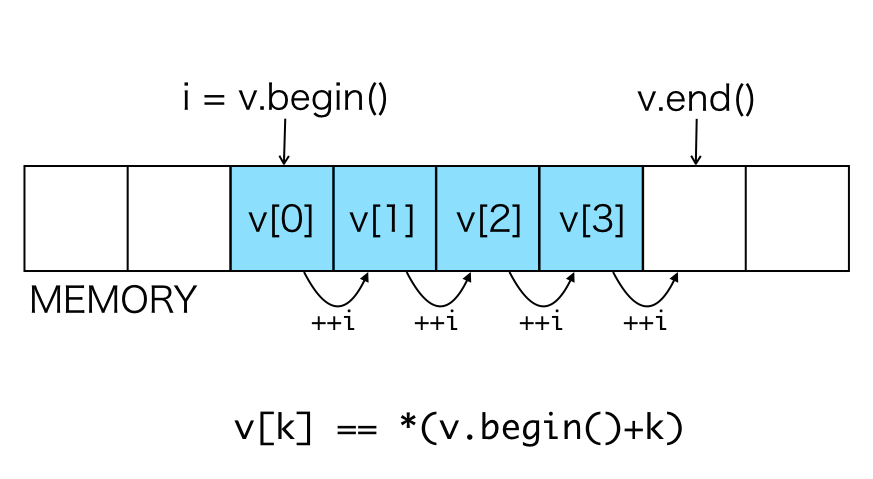
\includegraphics{iterator.png}

\begin{itemize}
\tightlist
\item
  \texttt{i\ =\ v.begin()} とするとイテレータ \texttt{i} は \texttt{v} の先頭要素を指し示します。
\item
  \texttt{++i} は、i を1つ次の要素を指す状態に更新します。
\item
  \texttt{-\/-i} は、i を1つ前の要素を指す状態に更新します。
\item
  \texttt{i+1} は、i の1つ次の要素を指し示すイテレータを表します。
\item
  \texttt{i-1} は、i の1つ前の要素を指し示すイテレータを表します。
\item
  \texttt{*i} は、i が指し示す要素の値を表します。
\item
  \texttt{v.end()} は \texttt{v} の末尾(最後の要素の1つ後)を指し示すイテレータを表します。
\item
  \texttt{*(v.begin()+k)} は v の k 番目の要素の値(\texttt{v{[}k{]}})を表します。
\end{itemize}

次のコード例は、イテレータを使って \texttt{NumericVector}の全ての要素を走査して値の合計値を求める例を示しています。

\begin{Shaded}
\begin{Highlighting}[]
\CommentTok{// [[Rcpp::export]]}
\DataTypeTok{double}\NormalTok{ rcpp_sum(NumericVector x) \{}
  \DataTypeTok{double}\NormalTok{ total = }\DecValTok{0}\NormalTok{;}
  \ControlFlowTok{for}\NormalTok{(NumericVector::iterator i = x.begin(); i != x.end(); ++i) \{}
\NormalTok{    total += *i;}
\NormalTok{  \}}
  \ControlFlowTok{return}\NormalTok{ total;}
\NormalTok{\}}
\end{Highlighting}
\end{Shaded}

\hypertarget{-c-}{%
\chapter{標準 C++ のデータ構造を利用する}\label{-c-}}

標準 C++ では \texttt{vector} \texttt{list} \texttt{map} \texttt{set} などの様々なデータ構造(コンテナ)が提供されています。それらはデータへのアクセス・追加・削除などの効率が異なるので、目的に応じて使い分けることで、実現したい処理をより効率よく実装できる場合があります。

例えば、ベクトルに要素を追加する処理を例にすると、Rcpp の \texttt{Rcpp::Vector} と標準 C++ の \texttt{std::vector} には、どちらにもベクトルの末尾に要素を追加するメンバ関数 \texttt{push\_back()} が提供されていますが、その処理効率には大きな違いがあります。なぜなら \texttt{Rcpp::Vector} では \texttt{push\_back()} メンバ関数を実行する度に追加した値を含むベクトル全体の値をメモリ上の他の場所にコピーする処理が発生するのに対して、\texttt{std::vector} では多くの場合には全体のコピーを行うことなく末尾に要素を追加することができるためです。

下に、\texttt{std::vector} を用いた例として、行列の要素の値が 0 ではない要素の行番号と列番号を取得する例を示します。

\begin{Shaded}
\begin{Highlighting}[]
\CommentTok{// [[Rcpp::export]]}
\NormalTok{DataFrame matix_rows_cols(NumericMatrix m)\{}
    \CommentTok{// 行列から値が 0 ではない要素の列番号と行番号を返します。}
    \CommentTok{// 簡単のため行列は NA を含まない前提とします。}

    \CommentTok{// 行数 I 、列数 J}
    \DataTypeTok{int}\NormalTok{ I = m.rows();}
    \DataTypeTok{int}\NormalTok{ J = m.cols();}

    \CommentTok{// 結果を標準 C++ コンテナの vector に格納します。}
    \BuiltInTok{std::}\NormalTok{vector<}\DataTypeTok{int}\NormalTok{> rows, cols; }\CommentTok{//行番号と列番号を格納する変数}

    \CommentTok{// 要素の数は最大で行列 m の要素数になり得るので}
    \CommentTok{// その分のメモリを先に確保します。}
\NormalTok{    rows.reserve(m.length());}
\NormalTok{    cols.reserve(m.length());}

    \CommentTok{// 行列 m の全ての要素にアクセスして}
    \CommentTok{// 値が 0 ではない要素の行番号と列番号を保存します。}
    \ControlFlowTok{for}\NormalTok{(}\DataTypeTok{int}\NormalTok{ i=}\DecValTok{0}\NormalTok{; i<I; ++i)\{}
        \ControlFlowTok{for}\NormalTok{(}\DataTypeTok{int}\NormalTok{ j=}\DecValTok{0}\NormalTok{; j<J; ++j)\{}
            \ControlFlowTok{if}\NormalTok{(m(i,j)!=}\FloatTok{0.0}\NormalTok{)\{}
\NormalTok{                rows.push_back(i}\DecValTok{+1}\NormalTok{);}
\NormalTok{                cols.push_back(j}\DecValTok{+1}\NormalTok{);}
\NormalTok{            \}}
\NormalTok{        \}}
\NormalTok{    \}}

    \CommentTok{// 結果をデータフレームとして返します。}
    \ControlFlowTok{return}\NormalTok{ DataFrame::create(Named(}\StringTok{"rows"}\NormalTok{, rows),}
\NormalTok{                             Named(}\StringTok{"cols"}\NormalTok{, cols));}
\NormalTok{\}}
\end{Highlighting}
\end{Shaded}

下に、いくつかの主要な標準 C++ データ構造の概要を示します。

\begin{longtable}[]{@{}cl@{}}
\toprule
標準 C++ データ構造 & 概要\tabularnewline
\midrule
\endhead
\texttt{vector} & 可変長配列:各要素はメモリ上で連続して配置されます。\tabularnewline
\texttt{list} & 可変長配列:各要素はメモリ上で分散して配置されます。\tabularnewline
\texttt{map}, \texttt{unordered\_map} & 連想配列:キー・バリュー形式でデータを保持します。\tabularnewline
\texttt{set}, \texttt{unordered\_set} & 集合:重複のない値の集合を保持します。\tabularnewline
\bottomrule
\end{longtable}

\texttt{map} は要素がキーの値でソートされた順に並びます。それに対して \texttt{unordered\_map} では順番は保証されませんが要素の挿入とアクセスの速度に優ります。同様に、\texttt{set} は要素の値でソートされた順に並びます。\texttt{unordered\_set} では順番は保証されませんが要素の挿入とアクセスの速度に優ります。

\hypertarget{-c--rcpp-}{%
\section{標準 C++ データ構造と Rcpp データ構造の変換}\label{-c--rcpp-}}

Rcpp のデータ構造と標準 C++ のデータ構造の変換には \texttt{as\textless{}T\textgreater{}()} 関数と \texttt{wrap()} 関数を用います。

\begin{itemize}
\tightlist
\item
  \texttt{as\textless{}CPP\textgreater{}(RCPP)} : Rcpp データ構造(RCPP)を標準 C++ データ構造(CPP)に変換します
\item
  \texttt{wrap(CPP)} : 標準 C++ データ構造(CPP)を Rcpp データ構造に変換します
\end{itemize}

下表に Rcpp と標準 C++ で変換可能なデータ構造の対応を示します。(\texttt{+} は対応している、\texttt{-} 対応していないことを示しています。)

\begin{longtable}[]{@{}cccc@{}}
\toprule
Rcpp & 標準 C++ & as & wrap\tabularnewline
\midrule
\endhead
\texttt{Vector} & \texttt{vector}, \texttt{list}, \texttt{deque} & + & +\tabularnewline
\texttt{List}, \texttt{DataFrame} & \texttt{vector\textless{}vector\textgreater{}}, \texttt{list\textless{}vector\textgreater{}} など & + & +\tabularnewline
名前付き \texttt{Vector} & \texttt{map}, \texttt{unordered\_map} & - & +\tabularnewline
\texttt{Vector} & \texttt{set}, \texttt{unordered\_set} & - & +\tabularnewline
\bottomrule
\end{longtable}

次のコード例では、Rcpp の \texttt{Vector} と標準 C++ のシーケンス・コンテナ( \texttt{vector}, \texttt{list}, \texttt{deque} など値が直列に並んでいるように扱えるコンテナ)を変換する例を示します。

\begin{Shaded}
\begin{Highlighting}[]
\NormalTok{NumericVector   rcpp_vector = \{}\DecValTok{1}\NormalTok{,}\DecValTok{2}\NormalTok{,}\DecValTok{3}\NormalTok{,}\DecValTok{4}\NormalTok{,}\DecValTok{5}\NormalTok{\};}

\CommentTok{// Rcpp::Vector から std::vector への変換  }
\BuiltInTok{std::}\NormalTok{vector<}\DataTypeTok{double}\NormalTok{>  cpp_vector = as< }\BuiltInTok{std::}\NormalTok{vector<}\DataTypeTok{double}\NormalTok{> >(rcpp_vector);}

\CommentTok{// std::vector から Rcpp::Vector への変換  }
\NormalTok{NumericVector v1 = wrap(cpp_vector);}
\end{Highlighting}
\end{Shaded}

次のコード例では、標準 C++ のシーケンス・コンテナが入れ子になった2次元コンテナを \texttt{DataFrame} や \texttt{List} に変換する例を示します。

\begin{Shaded}
\begin{Highlighting}[]
\CommentTok{//}
\KeywordTok{using} \KeywordTok{namespace}\NormalTok{ std;}

\CommentTok{// 要素となるベクトルの長さが全て等しい2次元ベクトルは}
\CommentTok{// DataFrame に変換できます}
\NormalTok{vector<vector<}\DataTypeTok{double}\NormalTok{>> cpp_vector_2d_01 = \{\{}\DecValTok{1}\NormalTok{,}\DecValTok{2}\NormalTok{\},\{}\DecValTok{3}\NormalTok{,}\DecValTok{4}\NormalTok{\}\};}
\NormalTok{DataFrame df = wrap(cpp_vector_2d_01);}

\CommentTok{// 要素となるベクトルの長さが異なる2次元ベクトルは}
\CommentTok{// List に変換できます}
\NormalTok{vector<vector<}\DataTypeTok{double}\NormalTok{>> cpp_vector_2d_02 = \{\{}\DecValTok{1}\NormalTok{,}\DecValTok{2}\NormalTok{\},\{}\DecValTok{3}\NormalTok{,}\DecValTok{4}\NormalTok{,}\DecValTok{5}\NormalTok{\}\};}
\NormalTok{List li = wrap(cpp_vector_2d_02);}
\end{Highlighting}
\end{Shaded}

次のコード例では、標準 C++ の \texttt{map\textless{}key,\ value\textgreater{}} と \texttt{unordered\_map\textless{}key,\ value\textgreater{}} は \texttt{key} を要素の名前、\texttt{value} を要素の型とした、名前付き Vector に変換されることを示します。

\begin{Shaded}
\begin{Highlighting}[]
\PreprocessorTok{#include}\ImportTok{<map>}
\CommentTok{// [[Rcpp::export]]}
\NormalTok{NumericVector std_map()\{}
    \BuiltInTok{std::}\NormalTok{map<}\BuiltInTok{std::}\NormalTok{string, }\DataTypeTok{double}\NormalTok{> cpp_num_map;}
\NormalTok{    cpp_num_map[}\StringTok{"C"}\NormalTok{] = }\DecValTok{3}\NormalTok{;    }
\NormalTok{    cpp_num_map[}\StringTok{"B"}\NormalTok{] = }\DecValTok{2}\NormalTok{;}
\NormalTok{    cpp_num_map[}\StringTok{"A"}\NormalTok{] = }\DecValTok{1}\NormalTok{;}

    \BuiltInTok{std::}\NormalTok{un<}\BuiltInTok{std::}\NormalTok{string, }\DataTypeTok{double}\NormalTok{> cpp_num_map;}
\NormalTok{    cpp_num_map[}\StringTok{"C"}\NormalTok{] = }\DecValTok{3}\NormalTok{;    }
\NormalTok{    cpp_num_map[}\StringTok{"B"}\NormalTok{] = }\DecValTok{2}\NormalTok{;}
\NormalTok{    cpp_num_map[}\StringTok{"A"}\NormalTok{] = }\DecValTok{1}\NormalTok{;}

\NormalTok{    Listli li = List::create(cpp_num_map, cpp_num_map);}
\NormalTok{\}}
\end{Highlighting}
\end{Shaded}

実行結果

\texttt{std::map} ではキーの値でソートされているのに対して、\texttt{std::unordered\_map} では順番が保証されないことがわかります。

\begin{verbatim}
> std_map()
[[1]]
A B C
2 1 3

[[2]]
A C B
2 3 1
\end{verbatim}

\hypertarget{-c-}{%
\section{標準 C++ データ構造を関数の引数や返値にする}\label{-c-}}

\texttt{as()} 関数や \texttt{wrap()} 関数で変換可能な標準 C++ データ構造は Rcpp 関数の引数や返値にすることもできます。そこでは R から Rcpp で記述した関数に値が渡される時、暗黙的に \texttt{as()} が呼ばれ、関数の返値が R に戻されるときには暗黙的に wrap() が呼ばれてデータが変換されます。

\begin{Shaded}
\begin{Highlighting}[]
\CommentTok{// [[Rcpp::plugins("cpp11")]]}
\CommentTok{// [[Rcpp::export]]}
\NormalTok{vector<}\DataTypeTok{double}\NormalTok{> times_two_std_vector(vector<}\DataTypeTok{double}\NormalTok{> v)\{ }\CommentTok{//暗黙的に as() が呼ばれる}
    \ControlFlowTok{for}\NormalTok{(}\DataTypeTok{double}\NormalTok{ &x : v)\{}
\NormalTok{        x *= }\DecValTok{2}\NormalTok{;}
\NormalTok{    \}}
    \ControlFlowTok{return}\NormalTok{ v; }\CommentTok{//暗黙的に wrap() が呼ばれる}
\NormalTok{\}}
\end{Highlighting}
\end{Shaded}

\hypertarget{-c-}{%
\chapter{標準 C++ アルゴリズム}\label{-c-}}

標準 C++ の \texttt{\textless{}algorithm\textgreater{}} と \texttt{\textless{}numeric\textgreater{}} ヘッダファイルでは様々な汎用アルゴリズムが提供されています。イテレータの章でも述べたように、その多くでは、イテレータを使ってアルゴリズムを適用する位置や範囲を指定します。

下のコード例では \texttt{\textless{}algorithm\textgreater{}} ヘッダファイルにある \texttt{count()} 関数を用いて、ベクトルに対して指定した値と等しい要素の数を数える例を示します。

\begin{verbatim}
#include <algorithm>
// [[Rcpp::export]]
int rcpp_count(){
    // 文字列ベクトルの作成
    CharacterVector v =
        CharacterVector::create("A", "B", "A", "C", NA_STRING);

    // 文字列ベクトル v から値が "A" である要素の数を数えます
    return std::count(v.begin(), v.end(), "A"); // 2
}
\end{verbatim}

なお、標準 C++ のクラスや関数などは \texttt{std::} 名前空間の中で定義されているため \texttt{std::vector} のように \texttt{std::} をつけて指定するか、 \texttt{using\ namespace\ std;} を記述して \texttt{std} 名前空間を利用するように指定します。

\hypertarget{boost-}{%
\chapter{Boost を利用する}\label{boost-}}

Boost ライブラリには標準 C++ よりもさらに先進的な機能が提供されています。
Boost ライブラリのうち、ヘッダー・ファイル・オンリーで使えるものについては、R のパッケージ \texttt{BH} をインストールすることで Rcpp でも利用できるようになります。

\begin{verbatim}
install.packages("BH")
\end{verbatim}

自分でインストールした Boost についても、ヘッダーとライブラリーへのパスを指定すれば利用できます。

\begin{verbatim}
Sys.setenv("PKG_CXXFLAGS"="-std=c++11 -I/opt/local/include -L/opt/local/lib/")
\end{verbatim}

コード例:

例:乱数生成器

\begin{verbatim}
#include <boost/random.hpp>
#include <boost/generator_iterator.hpp>
#include <boost/random/normal_distribution.hpp>

// [[Rcpp::export]]
NumericVector boostNormals(int n) {

typedef boost::mt19937 RNGType;   // select a generator, MT good default
RNGType rng(123456);            // instantiate and seed

boost::normal_distribution<> n01(0.0, 1.0);
boost::variate_generator< RNGType, boost::normal_distribution<> > rngNormal(rng, n01);

NumericVector V(n);
for ( int i = 0; i < n; i++ ) {
V[i] = rngNormal();
};

return V;
}
\end{verbatim}

R, Rcpp, C++11, Boost で乱数生成器のパフォーマンス比較

Rの乱数生成器を呼び出す

\begin{Shaded}
\begin{Highlighting}[]
\PreprocessorTok{#include }\ImportTok{<Rcpp.h>}
\KeywordTok{using} \KeywordTok{namespace}\NormalTok{ Rcpp;}
\CommentTok{// [[Rcpp::export]]}
\NormalTok{NumericVector rcppNormals(}\DataTypeTok{int}\NormalTok{ n) \{}
\ControlFlowTok{return}\NormalTok{ rnorm(n);}
\NormalTok{\}}
\end{Highlighting}
\end{Shaded}

ベンチマーク

\begin{verbatim}
library(rbenchmark)
n <- 10000
res <- benchmark(rcppNormals(n),
boostNormals(n),
cxx11Normals(n),
rnorm(n),
order="relative",
replications = 500)
print(res[,1:4])
\end{verbatim}

結果

\begin{verbatim}
test replications elapsed relative
2 boostNormals(n)          500   0.402    1.000
3 cxx11Normals(n)          500   0.425    1.057
1  rcppNormals(n)          500   0.505    1.256
4        rnorm(n)          500   0.675    1.679
\end{verbatim}

C++11やBoost のネイティブ乱数生成器が早いが、Rcpp版も健闘しています。どれも、ただのR関数よりは早い。

\begin{Shaded}
\begin{Highlighting}[]
\PreprocessorTok{#include }\ImportTok{<Rcpp.h>}

\CommentTok{// [[Rcpp::depends(BH)]]}

\CommentTok{// One include file from Boost}
\PreprocessorTok{#include }\ImportTok{<boost/date_time/gregorian/gregorian_types.hpp>}

\KeywordTok{using} \KeywordTok{namespace} \ExtensionTok{boost::}\NormalTok{gregorian;}

\CommentTok{// [[Rcpp::export]]}
\NormalTok{Rcpp::Date getIMMDate(}\DataTypeTok{int}\NormalTok{ mon, }\DataTypeTok{int}\NormalTok{ year) \{}
\CommentTok{// compute third Wednesday of given month / year}
\NormalTok{date d = nth_day_of_the_week_in_month(nth_day_of_the_week_in_month::third,}
\NormalTok{Wednesday, mon).get_date(year);}
\NormalTok{date::}\DataTypeTok{ymd_type}\NormalTok{ ymd = d.year_month_day();}
\ControlFlowTok{return}\NormalTok{ Rcpp::wrap(Rcpp::Date(ymd.year, ymd.month, ymd.day));}
\NormalTok{\}}
\end{Highlighting}
\end{Shaded}

IMM date は、毎月の3番目の水曜日のことを指す。Boost には mon 月 の N 週目の M 曜日を返す関数があります。\texttt{nth\_day\_of\_the\_week\_in\_month(M,\ N,\ mon)}

\begin{Shaded}
\begin{Highlighting}[]
\KeywordTok{getIMMDate}\NormalTok{(}\DecValTok{3}\NormalTok{, }\DecValTok{2013}\NormalTok{)}
\end{Highlighting}
\end{Shaded}

\hypertarget{rcpp}{%
\chapter{Rcppを用いたパッケージ作成}\label{rcpp}}

このセクションでは自作のパッケージで Rcpp を利用する方法を解説します。

\url{http://dirk.eddelbuettel.com/code/rcpp/Rcpp-package.pdf}

通常のユーザーはパッケージを作成する必要はないと考えるかもしれません。しかし、Rcpp で書いた関数はパッケージとして保存しておくことを薦めます。なぜなら、パッケージ化しないでRcppで作成した関数を利用する場合には、毎回 \texttt{sourceCppRcpp} でコンパイルしてRにロードする必要があります。それに対して、パッケージ化すると、コンパイル済みのRcpp関数を保存しておき、使うときには \texttt{library()} でロードするだけで済むようになるためです。

\hypertarget{rcpp}{%
\section{Rcppを用いたパッケージ作成の手順}\label{rcpp}}

\hypertarget{-rcpp-}{%
\subsection{手動で自作パッケージを Rcpp に対応させる}\label{-rcpp-}}

自作パッケージを手動で設定する方法を以下に示します。(作成しているパッケージの名前を \texttt{myPackage} とします。)

\begin{itemize}
\tightlist
\item
  src/ フォルダを作成する
\end{itemize}

C/C++ のソース・ファイルはこのフォルダの中に配置します。

\begin{itemize}
\tightlist
\item
  \texttt{DESCRIPTION}ファイルに以下の記述を追加する
\end{itemize}

\begin{verbatim}
LinkingTo: Rcpp
Imports: Rcpp
\end{verbatim}

\texttt{LinkingTo:} は、ここで指定したパッケージが提供するC/C++のヘッダファイルを、自作パッケージから利用できるようにします。

\texttt{Imports:} は、ここで指定したパッケージが提供するRの関数を、この自作パッケージから利用可能にします。また、この自作パッケージがここで指定したパッケージに依存していることを明示します。

(\texttt{Depends:} も、ここで指定したパッケージが提供するRの関数を、この自作パッケージから利用可能にします。Importとの違いは、この自作パッケージをRにlibrary()でロードしたときに、ここで指定したパッケージもlibrary()でロードされるということ。)

\begin{itemize}
\tightlist
\item
  \texttt{NAMESPACE}ファイルに以下の記述を追加する
\end{itemize}

\begin{verbatim}
useDynLib(myPackage, .registration=TRUE)
exportPattern("^[[:alpha:]]+")
importFrom(Rcpp, sourceCpp)
\end{verbatim}

\texttt{useDynLib(myPackage)}は、この自作パッケージ自身に含まれるコンパイルされた関数を、この自作パッケージ自身の R 関数から利用可能にします。(このパッケージのコンパイルされた関数のポインタ(アドレス)がこのパッケージのRの関数からアクセスできるようにする?)

\texttt{exportPattern("\^{}{[}{[}:alpha:{]}{]}+")} は、このパッケージで定義された R の関数のうち、どれをパッケージのユーザーから利用できるようにするか指定しています。ここでは正規表現を使って全ての関数を指定しています。(Rcppを使うと \texttt{//\ {[}{[}Rcpp::export{]}{]}} を付けて定義した C++ の関数と同名の R の関数が自動で作成される。それを \texttt{exportPattern("\^{}{[}{[}:alpha:{]}{]}+")} によって、全てをRから利用可能にしている)。ちなみに \texttt{export(foo,\ bar)} とすると定義されたRの関数 \texttt{foo} と \texttt{bar} のみがユーザーから利用可能になります。

\texttt{importFrom(Rcpp,\ sourceCpp)} は、このパッケージ内の R の関数から、Rcpp パッケージの \texttt{sourceCpp} 関数を \texttt{::} なしで呼び出し可能にしています。(このパッケージ内で \texttt{sourceCpp} と書くと \texttt{Rcpp::sourceCpp} と解釈される )。ちなみに \texttt{import(foo,\ bar)} と書くと、このパッケージの内部でパッケージ \texttt{foo} と \texttt{bar} の全ての関数が \texttt{::} なしで呼び出し可能になります。これはこのパッケージの中で \texttt{library()} を使ったのと同じ効果を持ちます。しかし \texttt{import()} を使って他のパッケージの関数を自作パッケージ内から利用可能にすることはできる限り避けた方が良いでしょう。その理由は2つあって、1つは他のパッケージと関数名の衝突が起こる恐れがあること、もう1つは、利用している関数のどれがどのパッケージの物なのかわかりにくくなるためです。

自作パッケージの中で他のパッケージの関数を利用する場合は、 \texttt{DESCRIPTION} ファイルの \texttt{Imports:} フィールドに他のパッケージを指定し、自作関数内では \texttt{パッケージ名::関数名} の形式で利用するのが良いでしょう。どうしても必要なもの(例えば \texttt{dplyr::"\%\textgreater{}\%"} など)だけ \texttt{NAMESPACE} ファイルで \texttt{importfrom(dplyr,\ "\%\textgreater{}\%")} で加えましょう。

\hypertarget{rcpp.package.skeleton-}{%
\subsection{Rcpp.package.skeleton() を利用する}\label{rcpp.package.skeleton-}}

Rcppを用いたパッケージを新規に作成する際に、最も簡単な方法は \texttt{Rcpp::Rcpp.package.skeleton()} を用いる方法です。

\begin{verbatim}
Rcpp.package.skeleton(
  # パッケージ名
  name = "anRpackage",
  # パッケージに含めたいオブジェクトの名前(文字列ベクトルで指定)
  list = character(),
  # 引数 list で指定したオブジェクトを探す環境
  environment = .GlobalEnv,
  # 作成するパッケージのフォルダの保存先
  path = ".",
  # TRUEなら既存のパッケージのフォルダを上書きする
  force = FALSE,
  # パッケージに含めたいコードが書かれたRファイルへのパスを指定する
  code_files = character(),
  # パッケージに含めたいコードが書かれたC++ファイルへのパスを指定する
  cpp_files = character(),
  # TRUEならRcppを用いたC++コード例をパッケージに追加する
    example_code = TRUE,
  # TRUEならパッケージに含めるC++コード例は Rcpp attributes を利用する
  attributes = TRUE,
  # TRUEなら作成するパッケージの雛形にModuleの例を含める
  module = FALSE,
  # パッケージの著者
    author = "Your Name"
  # パッケージのメンテナー
    maintainer = if(missing( author)) "Your Name" else author,
  # パッケージのメンテナーのメールアドレス
    email = "your@email.com",
  # パッケージのライセンス
    license = "GPL (>= 2)"
    )
\end{verbatim}

使用例

\begin{verbatim}
Rcpp::Rcpp.package.skeleton("myPackage")
\end{verbatim}

上のコードを実行すると myRcppPackage というパッケージのフォルダが作成されます。

\hypertarget{devtoolsuse_rcpp-}{%
\subsection{devtools::use\_rcpp() を用いる}\label{devtoolsuse_rcpp-}}

既存の自作パッケージに Rcpp を利用した関数を追加したい場合には、\texttt{devtools::use\_rcpp()} を利用する方法もあります。

\begin{verbatim}
use_rcpp(
  # パッケージのフォルダへのパスを指定する
  pkg = "." 
  )
\end{verbatim}

次の例では、最初に \texttt{package.skeleton()} でパッケージの雛形を作成してから、\texttt{devtools::use\_rcpp()} でそのパッケージをRcppを利用するために必要な設定を行っています。

\begin{verbatim}
> package.skeleton("myPackage")
Creating directories ...
Creating DESCRIPTION ...
Creating NAMESPACE ...
Creating Read-and-delete-me ...
Saving functions and data ...
Making help files ...
Done.
Further steps are described in './myPackage/Read-and-delete-me'.

> devtools::use_rcpp("myPackage")
Adding Rcpp to LinkingTo and Imports
* Creating `src/`.
* Ignoring generated binary files.
Next, include the following roxygen tags somewhere in your package:

#' @useDynLib myPackage, .registration=TRUE
#' @importFrom Rcpp sourceCpp
NULL

Then run document()
\end{verbatim}

この方法を用いた場合には、\texttt{NAMESPACE} には設定が追加されません。そこで、このパッケージのRコードのどこかに次の記述を追加してから \texttt{devtools::document()}を実行します。
詳しくは次のセクションを参照ください。

\begin{verbatim}
#' @useDynLib myPackage, .registration=TRUE
#' @importFrom Rcpp sourceCpp
NULL
\end{verbatim}

\hypertarget{roxygen2-}{%
\section{roxygen2 パッケージを用いてパッケージのパッケージのドキュメントを作成する}\label{roxygen2-}}

RコードやC++コードの中にroxygenタグと呼ばれる特殊な文字列を記述することで、パッケージ関数のヘルプやNAMESPACEファイルの内容を生成させることができます。

roxygenタグからドキュメントのソースファイルを生成するには \texttt{devtools::document()} を実行します。

例えば、下の記述をパッケージ内のRコードのどこかに記述してから \texttt{devtools::document()} を実行すると、

\begin{verbatim}
#' @useDynLib myPackage, .registration=TRUE
#' @importFrom Rcpp sourceCpp
NULL
\end{verbatim}

\texttt{NAMESPACE} ファイルに次の記述が加えられます。

\begin{verbatim}
importFrom(Rcpp,sourceCpp)
useDynLib(myPackage)
\end{verbatim}

\hypertarget{cc}{%
\section{自作パッケージで他のパッケージのC/C++関数を利用する}\label{cc}}

Rのパッケージによっては、そのパッケージで定義されたC/C++の関数やクラスを他のパッケージから利用できるように公開しているものもあります。自作パッケージから、他のパッケージが公開しているパッケージを利用するには以下の方法を用います。

\hypertarget{cc}{%
\section{自作パッケージでサードパーティのC/C++ライブラリを利用する}\label{cc}}

\hypertarget{rcppparallel}{%
\chapter{RcppParallel}\label{rcppparallel}}

公式サイト:\url{http://rcppcore.github.io/RcppParallel/}

RcppParallel は Rcpp で並列プログラミングを可能にするパッケージ。バックエンドとして Windows, OS X, Linux では Intel Threaded Building Blocks (TBB) ライブラリ、その他のプラットフォームでは TinyThread ライブラリを用いています。

\#\#RcppParallelの並列化の特徴

Rには既に他にも parallel や snow など、多くの並列化パッケージあるが、RcppParallel 並列化との間には重要な違いが存在します。

parallel や snow での並列化は \textbf{マルチプロセス} の方式であり、複数のRを別プロセスとして立ち上げて並列で実行します。そのため、元のRから並列計算を行うRにデータを転送する必要があります。1台のコンピュータでのみ並列計算を行う際にも並列プロセス間で socket 通信を介してデータをコピーするため、データが大きい場合には転送に非常に時間がかかってしまう。

一方、RcppParallelでの並列化は \textbf{マルチスレッド} です。そのため、1台のコンピュータの複数コアでの並列計算しか行うことができない。しかし、並列スレッドは元のRとメモリ上のデータを共有できるため、データ転送のコストがかからない。そのため1台のPCしかない場合にはマルチスレッドのほうがアドバンテージは非常に大きくなります。

これまで、R や Rcpp のAPIを使ったマルチスレッド・プログラミングは技術的ハードルが高いため、使えるのはエキスパートに限られていた。しかし、RcppParallelを使うと、スレッド並列化に必要な処理
を全て自動で行ってくれるので、ユーザーは実現したい処理の実装に集中できます。

\hypertarget{-1}{%
\section{インストール}\label{-1}}

\begin{Shaded}
\begin{Highlighting}[]
\KeywordTok{install.packages}\NormalTok{(}\StringTok{"RcppParallel"}\NormalTok{)}
\KeywordTok{install_github}\NormalTok{(}\StringTok{"RcppParallel"}\NormalTok{,}\StringTok{"RcppCore"}\NormalTok{)}
\end{Highlighting}
\end{Shaded}

Rcppソースに以下を追加

\begin{Shaded}
\begin{Highlighting}[]
\CommentTok{// [[Rcpp::depends(RcppParallel)]]}
\PreprocessorTok{#include }\ImportTok{<RcppParallel.h>}
\end{Highlighting}
\end{Shaded}

\hypertarget{parallelfor-parallelreduce}{%
\subsection{parallelFor, parallelReduce}\label{parallelfor-parallelreduce}}

RcppParallel は \texttt{parallelFor()} と \texttt{parallelReduce()} の2つの関数を提供します。

\begin{Shaded}
\begin{Highlighting}[]
\DataTypeTok{void}\NormalTok{ parallelFor(}\BuiltInTok{std::}\NormalTok{size_t begin, }\BuiltInTok{std::}\NormalTok{size_t end, }
\NormalTok{                    Worker& worker, }\BuiltInTok{std::}\NormalTok{size_t grainSize = }\DecValTok{1}\NormalTok{)}
\DataTypeTok{void}\NormalTok{ parallelReduce(}\BuiltInTok{std::}\NormalTok{size_t begin, }\BuiltInTok{std::}\NormalTok{size_t end, }
\NormalTok{                        Reducer& reducer, }\BuiltInTok{std::}\NormalTok{size_t grainSize = }\DecValTok{1}\NormalTok{)}
\end{Highlighting}
\end{Shaded}

\texttt{parallelFor\textasciigrave{}\textasciigrave{}parallelReduce} は \texttt{Vector}と \texttt{Matrix} の \texttt{begin} から \texttt{end-1} までの要素に対して \texttt{worker} \texttt{reducer} で定義された処理を並列で実行します。

\textbf{parallelFor} は入力データの各要素と出力データの各要素が1対1で対応するような処理 (例えば sqrt() や log()) を並列化する場合に用います。

\textbf{parallelReduce} は入力データの全要素を1つの値に集約するような処理 (例えば sum()やmean()) を並列化する場合に用います。

現状の\texttt{RcppParallel(バージョン4.3.15)} では \texttt{parallelFor()} \texttt{parallelReduce()} は DataFrame のカラムや List の要素毎の並列化には対応していません。

\hypertarget{rvector-rmatrix}{%
\subsection{RVector, RMatrix}\label{rvector-rmatrix}}

マルチスレッド処理では、入力データや出力データの同じ要素に対して、異なる並列スレッドが同時にアクセスすることを防ぐ ``スレッドセーフ'' なデータアクセスが必要があります。

\texttt{RcppParallel} では Rcppの \texttt{Vector} や \texttt{Matrix} に対してスレッドセーフにアクセスするためのラッパー \texttt{RVector} \texttt{RMatrix}を提供しています。

\begin{Shaded}
\begin{Highlighting}[]
\CommentTok{//整数ベクターを RVector<int> に変換します。}
\NormalTok{IntegerVector v_int;}
\NormalTok{RVector<}\DataTypeTok{int}\NormalTok{> vp_int(v_int);}

\CommentTok{//実数行列を Rmatrix<double> に変換します。}
\NormalTok{NumericMatrix }\VariableTok{m_num}\NormalTok{;}
\NormalTok{Rmatrix<}\DataTypeTok{double}\NormalTok{> mp_num(}\VariableTok{m_num}\NormalTok{);}
\end{Highlighting}
\end{Shaded}

\hypertarget{worker}{%
\section{Worker}\label{worker}}

\texttt{parallelFor} \texttt{parallelReduce} で処理する内容は関数オブジェクトとして定義します。

\texttt{parallelFor\textasciigrave{}\textasciigrave{}parallelReduce} に渡す関数オブジェクトは \texttt{Worker} クラスを継承して作成します。

\hypertarget{parallelfor}{%
\section{例:parallelFor()}\label{parallelfor}}

\texttt{parallelFor} を使って、\texttt{Matrix} の各要素の平方根を計算します。
\url{http://gallery.rcpp.org/articles/parallel-matrix-transform/}

\begin{Shaded}
\begin{Highlighting}[]
\CommentTok{// [[Rcpp::depends(RcppParallel)]]}
\PreprocessorTok{#include }\ImportTok{<RcppParallel.h>}
\KeywordTok{using} \KeywordTok{namespace}\NormalTok{ RcppParallel;}

\CommentTok{// Worker を継承して関数オブジェクト SquareRoot を定義する}
\KeywordTok{struct}\NormalTok{ SquareRoot : }\KeywordTok{public}\NormalTok{ Worker}
\NormalTok{\{}
  \CommentTok{// 入力データを保持する内部変数}
  \AttributeTok{const}\NormalTok{ RMatrix<}\DataTypeTok{double}\NormalTok{> input_data;}
  
  \CommentTok{// 出力データを保持する内部変数}
\NormalTok{  RMatrix<}\DataTypeTok{double}\NormalTok{> output_data;}
  
  \CommentTok{//関数オブジェクトをインスタンス化するときに}
  \CommentTok{//入力データ・出力データを与えて内部変数を初期化する}
\NormalTok{  SquareRoot(}\AttributeTok{const}\NormalTok{ NumericMatrix input, NumericMatrix output) }
\NormalTok{    : input_data(input), output_data(output) \{\}}
  
  \CommentTok{// 関数オブジェクトの処理内容を定義する}
  \CommentTok{// parallelFor により、ある1つのスレッドで処理する範囲が}
  \CommentTok{// begin, end で与えられる }
  \DataTypeTok{void} \KeywordTok{operator}\NormalTok{()(}\BuiltInTok{std::}\NormalTok{size_t begin, }\BuiltInTok{std::}\NormalTok{size_t end) \{}
    \BuiltInTok{std::}\NormalTok{transform(input_data.begin() + begin,}
\NormalTok{                   input_data.begin() + end, }
\NormalTok{                   output_data.begin() + begin, }
\NormalTok{                   ::sqrt);}
\NormalTok{  \}}
\NormalTok{\};}


\CommentTok{// [[Rcpp::export]]}
\NormalTok{NumericMatrix parallelMatrixSqrt(NumericMatrix x) \{}
  
  \CommentTok{// 出力データを保存する Matrix を用意する}
\NormalTok{  NumericMatrix output(x.nrow(), x.ncol());}
  
  \CommentTok{// 関数オブジェクトをインスタンス化する}
  \CommentTok{// このとき入力データ、出力データを渡す}
\NormalTok{  SquareRoot my_sqrt(x, output);}
  
  \CommentTok{// parallelFor()を使って、}
  \CommentTok{// 入力データの全ての要素に対して関数オブジェクトを適用する}
  \CommentTok{// この中で output に値がセットされる}
\NormalTok{  parallelFor(}\DecValTok{0}\NormalTok{, x.length(), my_sqrt);}
  
  \CommentTok{// エラー:この記述は誤り parallelFor() の返値は void}
  \CommentTok{// output = parallelFor(0, x.length(), squareRoot);}
  
  \CommentTok{// 結果を出力}
  \ControlFlowTok{return}\NormalTok{ output;}
\NormalTok{\}}
\end{Highlighting}
\end{Shaded}

\hypertarget{parallelreduce}{%
\section{例:parallelReduce()}\label{parallelreduce}}

ベクターの要素の合計値を計算する
\url{http://gallery.rcpp.org/articles/parallel-vector-sum/}

\begin{Shaded}
\begin{Highlighting}[]
\CommentTok{// [[Rcpp::depends(RcppParallel)]]}
\PreprocessorTok{#include }\ImportTok{<RcppParallel.h>}
\KeywordTok{using} \KeywordTok{namespace}\NormalTok{ RcppParallel;}

\KeywordTok{struct}\NormalTok{ Sum : }\KeywordTok{public}\NormalTok{ Worker}
\NormalTok{\{   }
  \CommentTok{// 入力値}
  \AttributeTok{const}\NormalTok{ RVector<}\DataTypeTok{double}\NormalTok{> input_data;}
  
  \CommentTok{// 合計値}
  \CommentTok{// この変数の型は RVector<T> の要素の型 T と一致している必要がある}
  \DataTypeTok{double}\NormalTok{ value;}
  
  \CommentTok{//最初に入力データを取得するためのコンストラクタ}
\NormalTok{  Sum(}\AttributeTok{const}\NormalTok{ NumericVector input) : input_data(input), value(}\DecValTok{0}\NormalTok{) \{\}}
  \CommentTok{//分割された入力データ(sum.input_data)を受け取って、スレッドに渡すときに使われるコンストラクタ}
\NormalTok{  Sum(}\AttributeTok{const}\NormalTok{ Sum& sum, Split) : input_data(sum.input_data), value(}\DecValTok{0}\NormalTok{) \{\} }
  
  
  \CommentTok{// input_data の要素番号 begin から要素番号 (end - 1) までの要素の合計値を計算する }
  \DataTypeTok{void} \KeywordTok{operator}\NormalTok{()(}\BuiltInTok{std::}\NormalTok{size_t begin, }\BuiltInTok{std::}\NormalTok{size_t end) \{}
\NormalTok{    value += }\BuiltInTok{std::}\NormalTok{accumulate(input_data.begin() + begin, input_data.begin() + end, }\FloatTok{0.0}\NormalTok{);}
\NormalTok{  \}}
  
  \CommentTok{// 他のスレッドで計算された結果を、このスレッドで計算された結果と、合体させるための処理}
  \DataTypeTok{void}\NormalTok{ join(}\AttributeTok{const}\NormalTok{ Sum& rhs) \{ }
\NormalTok{    value += rhs.value; }
\NormalTok{  \}}
\NormalTok{\};}



\CommentTok{// [[Rcpp::export]]}
\DataTypeTok{double}\NormalTok{ parallelVectorSum(NumericVector x) \{}
  
  \CommentTok{// 入力データ x を渡して関数オブジェクトをインスタンス化}
\NormalTok{  Sum sum(x);}
  
  \CommentTok{// 要素番号 0 から x.length() -1 までの要素の合計を求める}
\NormalTok{  parallelReduce(}\DecValTok{0}\NormalTok{, x.length(), sum);}
  
  \CommentTok{// 合計値を返す}
  \ControlFlowTok{return}\NormalTok{ sum.value;}
\NormalTok{\}}
\end{Highlighting}
\end{Shaded}

\#\#パッケージで利用する場合

各ファイルに以下の記述を追加する

\textbf{DESCRIPTION}

\begin{verbatim}
Imports: RcppParallel
LinkingTo: RcppParallel
SystemRequirements: GNU make
\end{verbatim}

\textbf{NAMESPACE}

\begin{verbatim}
importFrom(RcppParallel, RcppParallelLibs)
\end{verbatim}

**src\Makevars**

\begin{verbatim}
PKG_LIBS += $(shell ${R_HOME}/bin/Rscript -e "RcppParallel::RcppParallelLibs()")
src\Makevars.win

PKG_CXXFLAGS += -DRCPP_PARALLEL_USE_TBB=1

PKG_LIBS += $(shell "${R_HOME}/bin${R_ARCH_BIN}/Rscript.exe" \
              -e "RcppParallel::RcppParallelLibs()")
\end{verbatim}

\chapter{リンク}

\begin{itemize}
\tightlist
\item
  \href{http://gallery.rcpp.org/}{Rcpp Gallery} : Rcpp を利用した様々なコード例が紹介されています。
\item
  \href{http://adv-r.had.co.nz/Rcpp.html}{Rcpp chapter in Advanced R} : Rcpp の基本的な使い方が簡潔にまとめられています。
\item
  \href{http://statr.me/rcpp-note/index.html}{Rcpp Note} :
  非公式な Rcpp のリファレンス作成プロジェクト
\item
  \href{http://dirk.eddelbuettel.com/code/rcpp/html/}{Rcpp Doxygen} : Rcpp のソースコードを参照できる
  *\href{https://cran.r-project.org/doc/manuals/r-release/R-ints.html}{R Internals} : R 内部の技術についての解説。SXEPなどRについてわからない単語が出てきたら、とりあえずこの文章を参照するとよいです。
\end{itemize}

\#パフォーマンス比較

RとRcppで記述した関数の実行速度を比較してみる。

\textbf{例:ギブス・サンプラー}

\url{http://gallery.rcpp.org/articles/gibbs-sampler/}

この例では、2重の for ループの中で乱数を生成し、結果を行列に格納しています。

\textbf{Rバージョン}

\begin{Shaded}
\begin{Highlighting}[]
\NormalTok{gibbsR <-}\StringTok{ }\ControlFlowTok{function}\NormalTok{(N,thin)\{}

\NormalTok{  mat<-}\KeywordTok{matrix}\NormalTok{(}\DecValTok{0}\NormalTok{,}\DataTypeTok{nrow=}\NormalTok{N,}\DataTypeTok{ncol=}\DecValTok{2}\NormalTok{)}
\NormalTok{  x <-}\StringTok{ }\DecValTok{0}
\NormalTok{  y <-}\StringTok{ }\DecValTok{0}

  \ControlFlowTok{for}\NormalTok{(i }\ControlFlowTok{in} \DecValTok{1}\OperatorTok{:}\NormalTok{N)\{}
    \ControlFlowTok{for}\NormalTok{(j }\ControlFlowTok{in} \DecValTok{1}\OperatorTok{:}\NormalTok{thin)\{}
\NormalTok{      x <-}\StringTok{ }\KeywordTok{rgamma}\NormalTok{(}\DecValTok{1}\NormalTok{, }\DecValTok{3}\NormalTok{, }\DecValTok{1}\OperatorTok{/}\NormalTok{(y}\OperatorTok{*}\NormalTok{y}\OperatorTok{+}\DecValTok{4}\NormalTok{))}
\NormalTok{      y <-}\StringTok{ }\KeywordTok{rnorm}\NormalTok{(}\DecValTok{1}\NormalTok{, }\DecValTok{1}\OperatorTok{/}\NormalTok{(x}\OperatorTok{+}\DecValTok{1}\NormalTok{), }\DecValTok{1}\OperatorTok{/}\KeywordTok{sqrt}\NormalTok{(}\DecValTok{2}\OperatorTok{*}\NormalTok{x}\OperatorTok{+}\DecValTok{2}\NormalTok{))}
\NormalTok{    \}}
\NormalTok{    mat[i,] <-}\StringTok{ }\KeywordTok{c}\NormalTok{(x,y)}
\NormalTok{  \}}
  \KeywordTok{return}\NormalTok{(mat)}
\NormalTok{\}}
\end{Highlighting}
\end{Shaded}

\textbf{Rcppバージョン}

以下のコードを ``gibbs.cpp'' というファイル名で保存します。

\begin{Shaded}
\begin{Highlighting}[]
\CommentTok{//gibbs.cpp}
\PreprocessorTok{#include }\ImportTok{<Rcpp.h>}
\KeywordTok{using} \KeywordTok{namespace}\NormalTok{ Rcpp;}

\CommentTok{// [[Rcpp::export]]}
\NormalTok{NumericMatrix gibbsCpp(}\DataTypeTok{int}\NormalTok{ N, }\DataTypeTok{int}\NormalTok{ thin) \{}

\NormalTok{  NumericMatrix mat(N, }\DecValTok{2}\NormalTok{);}
  \DataTypeTok{double}\NormalTok{ x = }\DecValTok{0}\NormalTok{, y = }\DecValTok{0}\NormalTok{;}

  \ControlFlowTok{for}\NormalTok{(}\DataTypeTok{int}\NormalTok{ i = }\DecValTok{0}\NormalTok{; i < N; i++) \{}
    \ControlFlowTok{for}\NormalTok{(}\DataTypeTok{int}\NormalTok{ j = }\DecValTok{0}\NormalTok{; j < thin; j++) \{}
\NormalTok{      x = R::rgamma(}\FloatTok{3.0}\NormalTok{, }\FloatTok{1.0}\NormalTok{ / (y * y + }\DecValTok{4}\NormalTok{));}
\NormalTok{      y = R::rnorm(}\FloatTok{1.0}\NormalTok{ / (x + }\DecValTok{1}\NormalTok{), }\FloatTok{1.0}\NormalTok{ / sqrt(}\DecValTok{2}\NormalTok{ * x + }\DecValTok{2}\NormalTok{));}
\NormalTok{    \}}
\NormalTok{    mat(i, }\DecValTok{0}\NormalTok{) = x;}
\NormalTok{    mat(i, }\DecValTok{1}\NormalTok{) = y;}
\NormalTok{  \}}

  \ControlFlowTok{return}\NormalTok{(mat);}
\NormalTok{\}}
\end{Highlighting}
\end{Shaded}

\textbf{コンパイル \& 実行}

\begin{Shaded}
\begin{Highlighting}[]
\KeywordTok{library}\NormalTok{(Rcpp)}
\KeywordTok{sourceCpp}\NormalTok{(}\StringTok{'gibbs.cpp'}\NormalTok{)}
\KeywordTok{gibbsCpp}\NormalTok{(}\DecValTok{100}\NormalTok{, }\DecValTok{10}\NormalTok{)}
\end{Highlighting}
\end{Shaded}

\textbf{R との比較}

RバージョンとRcppバージョンの関数の実行速度を比較してみる。その結果、Rcpp の方が56倍高速に実行されています。

この例のように、ベクターや行列の各要素への逐次アクセスするような場合に、Rcpp のアドバンテージが大きい。

\begin{Shaded}
\begin{Highlighting}[]
\KeywordTok{library}\NormalTok{(rbenchmark)}
\NormalTok{n <-}\StringTok{ }\DecValTok{2000}
\NormalTok{thn <-}\StringTok{ }\DecValTok{200}
\KeywordTok{benchmark}\NormalTok{( }\KeywordTok{gibbsR}\NormalTok{(n, thn),}
           \KeywordTok{gibbsCpp}\NormalTok{(n, thn),}
           \DataTypeTok{columns =} \KeywordTok{c}\NormalTok{(}\StringTok{"test"}\NormalTok{, }\StringTok{"replications"}\NormalTok{, }\StringTok{"elapsed"}\NormalTok{, }\StringTok{"relative"}\NormalTok{),}
           \DataTypeTok{order=}\StringTok{"relative"}\NormalTok{,}
           \DataTypeTok{replications=}\DecValTok{10}\NormalTok{)}
\end{Highlighting}
\end{Shaded}

実行結果

\begin{verbatim}
test  replications elapsed relative
   2     gibbsCpp(n, thn)           10   1.454    1.000
   1       gibbsR(n, thn)           10  81.427   56.002
\end{verbatim}

\hypertarget{rcpp-attributes}{%
\chapter{Rcpp Attributes}\label{rcpp-attributes}}

Rcpp Attributes はコンパイルに必要な情報をコンパイラに教えます。

\hypertarget{-rcpp-attributes}{%
\section{利用可能な Rcpp Attributes}\label{-rcpp-attributes}}

以下では、Rcppパッケージで利用可能な Rcpp Attributes の一覧とその機能を解説します。

\hypertarget{rcppexport}{%
\subsection{Rcpp::export}\label{rcppexport}}

\texttt{//\ {[}{[}Rcpp::export{]}{]}} を記述した直下で定義した C++ の関数は R から利用可能になります。

\texttt{//\ {[}{[}Rcpp::export{]}{]}} を記述した関数は \texttt{compileAttributes()} により処理され、改変された関数が \texttt{src/RcppExports.cpp} に生成されます。さらに、\texttt{src/RcppExports.cpp} で定義された C++ 関数を呼び出すRの関数が \texttt{R/RcppExports.R} に生成されます。

また、デフォルトでは C++ で定義した関数名と同名の関数がRで利用可能になります。しかし、C++の関数名の命名規約とRの関数の命名規約が異なるために、Rの関数名として利用できる文字のうち、C++の関数名としては利用できない文字(\texttt{.})もあります。その場合には下のように記述することで、Rで利用可能になる関数名を指定することができます。

\begin{verbatim}
// [[Rcpp::export(".myCppFunction")]]
\end{verbatim}

\begin{verbatim}
// [[Rcpp::export]]
int fibonacci(const int x) {

   if (x == 0) return(0);
   if (x == 1) return(1);

   return (fibonacci(x - 1)) + fibonacci(x - 2);
}

// [[Rcpp::export("convolveCpp")]]
NumericVector convolve(NumericVector a, NumericVector b) {

   int na = a.size(), nb = b.size();
   int nab = na + nb - 1;
   NumericVector xab(nab);

   for (int i = 0; i < na; i++)
      for (int j = 0; j < nb; j++)
         xab[i + j] += a[i] * b[j];

   return xab;
}
\end{verbatim}

\hypertarget{rcppinterfaces}{%
\section{Rcpp::interfaces}\label{rcppinterfaces}}

\begin{verbatim}
// [[Rcpp::interfaces(r, cpp)]]
\end{verbatim}

\hypertarget{rcppdepends}{%
\section{Rcpp::depends}\label{rcppdepends}}

\begin{verbatim}
// [[Rcpp::depends(RcppArmadillo)]]
// [[Rcpp::depends(Matrix, RcppGSL)]]
\end{verbatim}

\hypertarget{rcppplugins}{%
\section{Rcpp::plugins}\label{rcppplugins}}

\begin{verbatim}
// [[Rcpp::plugins(plugin1, plugin2)]]
// [[Rcpp::plugins(cpp11)]]
\end{verbatim}

\hypertarget{rcpp-attributes--rcpp-}{%
\section{Rcpp Attributes を処理する Rcpp の関数}\label{rcpp-attributes--rcpp-}}

\hypertarget{compileattributes}{%
\subsection{compileAttributes()}\label{compileattributes}}

ソースコード中の Rcpp Attributes を読み取り、定義した C++ 関数を呼び出す R 関数を自動で生成する。

\begin{verbatim}
compileAttributes(pkgdir = ".", verbose = getOption("verbose"))

\end{verbatim}

\chapter{書き加える可能性のある項目リスト}

RCPP\_RETURN\_VECTOR、RCPP\_RETURN\_MATRIX、Rcppの関数でポリモーフィズムを実現するためのマクロ。\href{http://gallery.rcpp.org/articles/rcpp-return-macros/}{参考}

NumericVectorベースの DatetimeVector DateVector の固有の機能、あれば

シュガー関数、 rowSums(), colSums(), rowMeans(), colMeans(), sample(), Arg(), upper\_tri(), lower\_tri(), trimws()

Added static methods eye(), ones(), and zeros() for select matrix types

Date and Datetime object and vector now have format methods and operator\textless{}\textless{} support

DataFrameの行数と列数のメソッドをMatrixと共通化されたらしい、.nrow(),.rows()、.ncol(),.cols()

Added printf-like syntax support for exception classes and variadic templating for Rcpp::stop and Rcpp::warning (James Balamuta in \#676).

New const iterators functions cbegin() and cend() have been added to several vector and matrix classes (Dan Dillon and James Balamuta in \#748) starting to address \#741).

New const iterators functions cbegin() and cend() added to MatrixRow as well (Dan Dillon in \#750). Matrix に ConstRow ConstColumn が追加された

Improve support for NVCC, the CUDA compiler (Iñaki Ucar in \#798 addressing \#797).

The `new' Date and Datetime vectors now have is\_na methods too. (Dirk in \#783 fixing \#781).

Added {[}{[}Rcpp::init{]}{]} attribute for registering C++ functions to run during package initialization (JJ in \#903 addressing \#902).

Added {[}{[}Rcpp::init{]}{]} attribute for registering C++ functions to run during package initialization (JJ in \#903 addressing \#902).

\chapter{済み}

シュガー関数、 rowSums(), colSums(), rowMeans(), colMeans(), sample()


\end{document}
